\documentclass[journal,12pt,twocolumn]{IEEEtran}
%
\usepackage{setspace}
\usepackage{gensymb}
%\doublespacing
\singlespacing

%\usepackage{graphicx}
%\usepackage{amssymb}
%\usepackage{relsize}
\usepackage[cmex10]{amsmath}
%\usepackage{amsthm}
%\interdisplaylinepenalty=2500
%\savesymbol{iint}
%\usepackage{txfonts}
%\restoresymbol{TXF}{iint}
%\usepackage{wasysym}
\usepackage{amsthm}
%\usepackage{iithtlc}
\usepackage{mathrsfs}
\usepackage{txfonts}
\usepackage{stfloats}
\usepackage{steinmetz}
\usepackage{bm}
\usepackage{cite}
\usepackage{cases}
\usepackage{subfig}
%\usepackage{xtab}
\usepackage{longtable}
\usepackage{multirow}
%\usepackage{algorithm}
%\usepackage{algpseudocode}
\usepackage{enumitem}
\usepackage{mathtools}
\usepackage{tikz}
\usepackage{circuitikz}
\usepackage{verbatim}
\usepackage{tfrupee}
\usepackage[breaklinks=true]{hyperref}
%\usepackage{stmaryrd}
\usepackage{tkz-euclide} % loads  TikZ and tkz-base
%\usetkzobj{all}
\usepackage{listings}
    \usepackage{color}                                            %%
    \usepackage{array}                                            %%
    \usepackage{longtable}                                        %%
    \usepackage{calc}                                             %%
    \usepackage{multirow}                                         %%
    \usepackage{hhline}                                           %%
    \usepackage{ifthen}                                           %%
  %optionally (for landscape tables embedded in another document): %%
    \usepackage{lscape}     
\usepackage{multicol}
\usepackage{chngcntr}
%\usepackage{enumerate}
\usepackage{blkarray}
%\usepackage{wasysym}
%\newcounter{MYtempeqncnt}
\DeclareMathOperator*{\Res}{Res}
%\renewcommand{\baselinestretch}{2}
\renewcommand\thesection{\arabic{section}}
\renewcommand\thesubsection{\thesection.\arabic{subsection}}
\renewcommand\thesubsubsection{\thesubsection.\arabic{subsubsection}}

\renewcommand\thesectiondis{\arabic{section}}
\renewcommand\thesubsectiondis{\thesectiondis.\arabic{subsection}}
\renewcommand\thesubsubsectiondis{\thesubsectiondis.\arabic{subsubsection}}

% correct bad hyphenation here
\hyphenation{op-tical net-works semi-conduc-tor}
\def\inputGnumericTable{}                                 %%

\lstset{
%language=C,
frame=single, 
breaklines=true,
columns=fullflexible
}
%\lstset{
%language=tex,
%frame=single, 
%breaklines=true
%}

\begin{document}
%


\newtheorem{theorem}{Theorem}[section]
\newtheorem{problem}{Problem}
\newtheorem{proposition}{Proposition}[section]
\newtheorem{lemma}{Lemma}[section]
\newtheorem{corollary}[theorem]{Corollary}
\newtheorem{example}{Example}[section]
\newtheorem{definition}[problem]{Definition}
%\newtheorem{thm}{Theorem}[section] 
%\newtheorem{defn}[thm]{Definition}
%\newtheorem{algorithm}{Algorithm}[section]
%\newtheorem{cor}{Corollary}
\newcommand{\BEQA}{\begin{eqnarray}}
\newcommand{\EEQA}{\end{eqnarray}}
\newcommand{\define}{\stackrel{\triangle}{=}}

\bibliographystyle{IEEEtran}
%\bibliographystyle{ieeetr}


\providecommand{\mbf}{\mathbf}
\providecommand{\pr}[1]{\ensuremath{\Pr\left(#1\right)}}
\providecommand{\qfunc}[1]{\ensuremath{Q\left(#1\right)}}
\providecommand{\sbrak}[1]{\ensuremath{{}\left[#1\right]}}
\providecommand{\lsbrak}[1]{\ensuremath{{}\left[#1\right.}}
\providecommand{\rsbrak}[1]{\ensuremath{{}\left.#1\right]}}
\providecommand{\brak}[1]{\ensuremath{\left(#1\right)}}
\providecommand{\lbrak}[1]{\ensuremath{\left(#1\right.}}
\providecommand{\rbrak}[1]{\ensuremath{\left.#1\right)}}
\providecommand{\cbrak}[1]{\ensuremath{\left\{#1\right\}}}
\providecommand{\lcbrak}[1]{\ensuremath{\left\{#1\right.}}
\providecommand{\rcbrak}[1]{\ensuremath{\left.#1\right\}}}
\theoremstyle{remark}
\newtheorem{rem}{Remark}
\newcommand{\sgn}{\mathop{\mathrm{sgn}}}
\providecommand{\abs}[1]{\left\vert#1\right\vert}
\providecommand{\res}[1]{\Res\displaylimits_{#1}} 
\providecommand{\norm}[1]{\left\lVert#1\right\rVert}
%\providecommand{\norm}[1]{\lVert#1\rVert}
\providecommand{\mtx}[1]{\mathbf{#1}}
\providecommand{\mean}[1]{E\left[ #1 \right]}
\providecommand{\fourier}{\overset{\mathcal{F}}{ \rightleftharpoons}}
%\providecommand{\hilbert}{\overset{\mathcal{H}}{ \rightleftharpoons}}
\providecommand{\system}{\overset{\mathcal{H}}{ \longleftrightarrow}}
	%\newcommand{\solution}[2]{\textbf{Solution:}{#1}}
\newcommand{\solution}{\noindent \textbf{Solution: }}
\newcommand{\cosec}{\,\text{cosec}\,}
\providecommand{\dec}[2]{\ensuremath{\overset{#1}{\underset{#2}{\gtrless}}}}
\newcommand{\myvec}[1]{\ensuremath{\begin{pmatrix}#1\end{pmatrix}}}
\newcommand{\mydet}[1]{\ensuremath{\begin{vmatrix}#1\end{vmatrix}}}
%\numberwithin{equation}{section}
\numberwithin{equation}{subsection}
%\numberwithin{problem}{section}
%\numberwithin{definition}{section}
\makeatletter
\@addtoreset{figure}{problem}
\makeatother

\let\StandardTheFigure\thefigure
\let\vec\mathbf
%\renewcommand{\thefigure}{\theproblem.\arabic{figure}}
\renewcommand{\thefigure}{\theproblem}
%\setlist[enumerate,1]{before=\renewcommand\theequation{\theenumi.\arabic{equation}}
%\counterwithin{equation}{enumi}


%\renewcommand{\theequation}{\arabic{subsection}.\arabic{equation}}

\def\putbox#1#2#3{\makebox[0in][l]{\makebox[#1][l]{}\raisebox{\baselineskip}[0in][0in]{\raisebox{#2}[0in][0in]{#3}}}}
     \def\rightbox#1{\makebox[0in][r]{#1}}
     \def\centbox#1{\makebox[0in]{#1}}
     \def\topbox#1{\raisebox{-\baselineskip}[0in][0in]{#1}}
     \def\midbox#1{\raisebox{-0.5\baselineskip}[0in][0in]{#1}}

\vspace{3cm}

\title{
	%\logo{
Matrix Analysis
	%}
}
\author{ G V V Sharma$^{*}$% <-this % stops a space
	\thanks{*The author is with the Department
		of Electrical Engineering, Indian Institute of Technology, Hyderabad
		502285 India e-mail:  gadepall@iith.ac.in. All content in this manual is released under GNU GPL.  Free and open source.}
	
}	
%\title{
%	\logo{Matrix Analysis through Octave}{\begin{center}\includegraphics[scale=.24]{tlc}\end{center}}{}{HAMDSP}
%}


% paper title
% can use linebreaks \\ within to get better formatting as desired
%\title{Matrix Analysis through Octave}
%
%
% author names and IEEE memberships
% note positions of commas and nonbreaking spaces ( ~ ) LaTeX will not break
% a structure at a ~ so this keeps an author's name from being broken across
% two lines.
% use \thanks{} to gain access to the first footnote area
% a separate \thanks must be used for each paragraph as LaTeX2e's \thanks
% was not built to handle multiple paragraphs
%

%\author{<-this % stops a space
%\thanks{}}
%}
% note the % following the last \IEEEmembership and also \thanks - 
% these prevent an unwanted space from occurring between the last author name
% and the end of the author line. i.e., if you had this:
% 
% \author{....lastname \thanks{...} \thanks{...} }
%                     ^------------^------------^----Do not want these spaces!
%
% a space would be appended to the last name and could cause every name on that
% line to be shifted left slightly. This is one of those "LaTeX things". For
% instance, "\textbf{A} \textbf{B}" will typeset as "A B" not "AB". To get
% "AB" then you have to do: "\textbf{A}\textbf{B}"
% \thanks is no different in this regard, so shield the last } of each \thanks
% that ends a line with a % and do not let a space in before the next \thanks.
% Spaces after \IEEEmembership other than the last one are OK (and needed) as
% you are supposed to have spaces between the names. For what it is worth,
% this is a minor point as most people would not even notice if the said evil
% space somehow managed to creep in.



% The paper headers
%\markboth{Journal of \LaTeX\ Class Files,~Vol.~6, No.~1, January~2007}%
%{Shell \MakeLowercase{\textit{et al.}}: Bare Demo of IEEEtran.cls for Journals}
% The only time the second header will appear is for the odd numbered pages
% after the title page when using the twoside option.
% 
% *** Note that you probably will NOT want to include the author's ***
% *** name in the headers of peer review papers.                   ***
% You can use \ifCLASSOPTIONpeerreview for conditional compilation here if
% you desire.




% If you want to put a publisher's ID mark on the page you can do it like
% this:
%\IEEEpubid{0000--0000/00\$00.00~\copyright~2007 IEEE}
% Remember, if you use this you must call \IEEEpubidadjcol in the second
% column for its text to clear the IEEEpubid mark.



% make the title area
\maketitle

\newpage

\tableofcontents

\bigskip

\renewcommand{\thefigure}{\theenumi}
\renewcommand{\thetable}{\theenumi}
%\renewcommand{\theequation}{\theenumi}

%\begin{abstract}
%%\boldmath
%In this letter, an algorithm for evaluating the exact analytical bit error rate  (BER)  for the piecewise linear (PL) combiner for  multiple relays is presented. Previous results were available only for upto three relays. The algorithm is unique in the sense that  the actual mathematical expressions, that are prohibitively large, need not be explicitly obtained. The diversity gain due to multiple relays is shown through plots of the analytical BER, well supported by simulations. 
%
%\end{abstract}
% IEEEtran.cls defaults to using nonbold math in the Abstract.
% This preserves the distinction between vectors and scalars. However,
% if the journal you are submitting to favors bold math in the abstract,
% then you can use LaTeX's standard command \boldmath at the very start
% of the abstract to achieve this. Many IEEE journals frown on math
% in the abstract anyway.

% Note that keywords are not normally used for peerreview papers.
%\begin{IEEEkeywords}
%Cooperative diversity, decode and forward, piecewise linear
%\end{IEEEkeywords}



% For peer review papers, you can put extra information on the cover
% page as needed:
% \ifCLASSOPTIONpeerreview
% \begin{center} \bfseries EDICS Category: 3-BBND \end{center}
% \fi
%
% For peerreview papers, this IEEEtran command inserts a page break and
% creates the second title. It will be ignored for other modes.
%\IEEEpeerreviewmaketitle

\begin{abstract}
This book provides a computational approach to school geometry based on the NCERT textbooks from Class 6-12.  Links to sample Python codes are available in the text.  
\end{abstract}
Download python codes using 
\begin{lstlisting}
svn co https://github.com/gadepall/school/trunk/ncert/computation/codes
\end{lstlisting}

\section{Examples}
\renewcommand{\theequation}{\theenumi}
\begin{enumerate}[label=\thesection.\arabic*.,ref=\thesection.\theenumi]
\numberwithin{equation}{enumi}

\input{./line/chem.tex}
%	
%\renewcommand{\theequation}{\theenumi}
%\begin{enumerate}[label=\arabic*.,ref=\thesubsection.\theenumi]
%\numberwithin{equation}{enumi}

\item Balance the following chemical equation.
%
\begin{align}
\label{eq:chem_balance}
Fe+H_2O &\rightarrow Fe_3O_4 + H_2
\end{align}
%
\solution Let the balanced version of \eqref{eq:chem_balance} be 
%
\begin{align}
\label{eq:chem_balance_unsol}
x_1Fe+x_2H_2 O &\rightarrow x_3Fe_3 O_4 + x_4H_2
\end{align}
%
which results in the following equations
%
\begin{align}
\begin{split}
\brak{x_1 -3x_3}Fe &= 0
\\
\brak{2x_2 -2x_4}H &= 0
\\
\brak{x_2 -4x_3}O &= 0
\end{split}
\end{align}
which can be expressed as
\begin{align}
\begin{split}
x_1 + 0.x_2 -3x_3 +0.x_4&= 0
\\
0.x_1+2x_2 +0.x_3-2x_4 &= 0
\\
0.x_1+x_2 -4x_3+ 0.x_4 &= 0
\end{split}
\end{align}
%
resulting in the matrix equation
\begin{align}
\label{eq:chem_balance_mat_eq}
\begin{split}
\myvec{
1 & 0 & -3 & 0
\\
0 & 2 & 0 & -2
\\
0 & 1 & -4 & 0
}
\vec{x} &= \vec{0}
\end{split}
\end{align}
%
where
\begin{align}
\vec{x} = \myvec{x_1 \\ x_2 \\ x_3 \\ x_4} 
\end{align}
%\item Solve \eqref{eq:chem_balance_unsol} by row reducing 
%the matrix in \eqref{eq:chem_balance_mat_eq}.
%\\
%\solution  
\eqref{eq:chem_balance_mat_eq} can be row reduced as follows
%
\begin{align}
\label{eq:chem_balance_mat_row}
\myvec{
1 & 0 & -3 & 0
\\
0 & 2 & 0 & -2
\\
0 & 1 & -4 & 0
}
 \xleftrightarrow[]{R_2 \leftarrow \frac{R_2}{2}}
\myvec{
1 & 0 & -3 & 0
\\
0 & 1 & 0 & -1
\\
0 & 1 & -4 & 0
}
\\
 \xleftrightarrow[]{R_3\leftarrow R_3-R_2}
\myvec{
1 & 0 & -3 & 0
\\
0 & 1 & 0 & -1
\\
0 & 0 & -4 & 1
}
\\
 \xleftrightarrow[]{R_1\leftarrow 4R_1-3R_3}
\myvec{
4 & 0 & 0 & -3
\\
0 & 1 & 0 & -1
\\
0 & 0 & -4 & 1
}
\\
 \xleftrightarrow[R_3 \leftarrow -\frac{1}{4}R_3]{R_1\leftarrow \frac{1}{4}}
\myvec{
1 & 0 & 0 & -\frac{3}{4}
\\
0 & 1 & 0 & -1
\\
0 & 0 & 1 & -\frac{1}{4}
}
\end{align}
%
Thus, 
\begin{align}
\label{eq:chem_balance_mat_sol}
x_1 &= \frac{3}{4}x_4, x_2 = x_4, x_3 = \frac{1}{4}x_4
\\
\\
\implies 
\vec{x} &= x_4\myvec{\frac{3}{4} \\ 1 \\ \frac{1}{4} \\ 1}= \myvec{3 \\ 4 \\ 1 \\ 4}
\end{align}
%
upon substituting $x_4 = 4$.
%
\eqref{eq:chem_balance_unsol} then becomes
%
\begin{align}
\label{eq:chem_balance_final}
3Fe+4H_2 O &\rightarrow Fe_3 O_4 + 4H_2
\end{align}

\item Consider the following information regarding the number of men and women workers in the three factories I,II and III

\begin{tabular}{ |c|c|c| } 
\hline
 & Men Workers & Women Workers \\
\hline
\multirow{3}{4em}{I \\II \\III} & 30 & 25\\ 
& 25 & 31 \\ 
&27 & 26 \\ 
\hline
\end{tabular}\\
Represent the above information in the form of a 3 $\times$ 2 matrix. What does the entry
in the third row and second column represent?\\


 \item  If a matrix has 8 elements, what are the possible orders it can have?\\
    \item Construct a 3 $\times$ 2 matrix whose elements are given by $a_{ij}=\frac{1}{2}\abs{i-3j}$\\
    \item \myvec{x+3 &z+4 &2y-7\\-6 &a-1 &0\\b-3 &-21 &0}=\myvec{0 &6 &3y-2\\-6 &-3 &2c+2\\2b+4 &-21 &0}\\
    Find the values of a,b,c,x,y and z.\\
\solution 
\input{./solutions/5/chapters/lines/docq7.tex}
    \item Find the values of a,b,c and d from the following equation:\\
    \myvec{2a+b &a-2b\\5c-d &4c+3d}=\myvec{4 &-3\\11 &24}\\
\solution 
%
\begin{align}
    E(X) &= \frac{1}{\sqrt{2\pi}} \int_{-\infty}^{\infty} x e^{-\frac{x^2}{2}}dx\\
    &=0 \quad \brak{ \text{ odd function}}
\end{align}
\begin{align}
    E\brak{X^2}&= \frac{1}{\sqrt{2\pi}}\int_{-\infty}^{\infty} x^2
e^ {-\frac{x^2}{2}} dx \quad \brak{even function}\\
    &= \frac{2}{\sqrt{2\pi}} \int_{0}^{\infty} x^2 e^{-\frac{x^2}{2}} dx\\
    &= \frac{2}{\sqrt{2\pi}}\int_{0}^{\infty}\sqrt{2u}e^{-u} du \quad\brak{Let \frac{x^2}{2}= u}\\
    &= \frac{2}{\sqrt{\pi}} \int_{0}^{\infty} e^{-u} u^{\frac{3}{2}-1} du\\
    &= \frac{2}{\sqrt{\pi}} \Gamma\brak{{\frac{3}{2}}}\\
    &= \frac{1}{\sqrt{\pi}}\Gamma\brak{\frac{1}{2}} \\
    &= 1
\end{align}
where we have used the fact that
\begin{align}
\quad\because \Gamma(n)= (n-1)\Gamma(n-1); \Gamma\brak{\frac{1}{2}}=\sqrt{\pi}
\end{align}
%
Thus, the  variance is
\begin{align}
    \sigma^2 =  E\brak X^2 - E^2\brak X = 1
\end{align}

    \item Given A=\myvec{\sqrt{3} &1 &-1\\2 &3 &0} and B=\myvec{2 &\sqrt{5} &1\\-2 &3 &\frac{1}{2}}, find A+B.\\\solution 
%
\begin{align}
    E(X) &= \frac{1}{\sqrt{2\pi}} \int_{-\infty}^{\infty} x e^{-\frac{x^2}{2}}dx\\
    &=0 \quad \brak{ \text{ odd function}}
\end{align}
\begin{align}
    E\brak{X^2}&= \frac{1}{\sqrt{2\pi}}\int_{-\infty}^{\infty} x^2
e^ {-\frac{x^2}{2}} dx \quad \brak{even function}\\
    &= \frac{2}{\sqrt{2\pi}} \int_{0}^{\infty} x^2 e^{-\frac{x^2}{2}} dx\\
    &= \frac{2}{\sqrt{2\pi}}\int_{0}^{\infty}\sqrt{2u}e^{-u} du \quad\brak{Let \frac{x^2}{2}= u}\\
    &= \frac{2}{\sqrt{\pi}} \int_{0}^{\infty} e^{-u} u^{\frac{3}{2}-1} du\\
    &= \frac{2}{\sqrt{\pi}} \Gamma\brak{{\frac{3}{2}}}\\
    &= \frac{1}{\sqrt{\pi}}\Gamma\brak{\frac{1}{2}} \\
    &= 1
\end{align}
where we have used the fact that
\begin{align}
\quad\because \Gamma(n)= (n-1)\Gamma(n-1); \Gamma\brak{\frac{1}{2}}=\sqrt{\pi}
\end{align}
%
Thus, the  variance is
\begin{align}
    \sigma^2 =  E\brak X^2 - E^2\brak X = 1
\end{align}

\item In the matrix A=\myvec{2 &5 &19 &-7\\ 35 &-2 &\frac{5}{2} &12 \\ \sqrt{3} &1 &-5 &17}, write
\begin{enumerate}
\item The order of the matrix
\item The number of elements
\item Write the elements $a_{31},a_{21},a_{33},a_{24},a_{23}.$
\end{enumerate}
\solution 
%
\begin{align}
    E(X) &= \frac{1}{\sqrt{2\pi}} \int_{-\infty}^{\infty} x e^{-\frac{x^2}{2}}dx\\
    &=0 \quad \brak{ \text{ odd function}}
\end{align}
\begin{align}
    E\brak{X^2}&= \frac{1}{\sqrt{2\pi}}\int_{-\infty}^{\infty} x^2
e^ {-\frac{x^2}{2}} dx \quad \brak{even function}\\
    &= \frac{2}{\sqrt{2\pi}} \int_{0}^{\infty} x^2 e^{-\frac{x^2}{2}} dx\\
    &= \frac{2}{\sqrt{2\pi}}\int_{0}^{\infty}\sqrt{2u}e^{-u} du \quad\brak{Let \frac{x^2}{2}= u}\\
    &= \frac{2}{\sqrt{\pi}} \int_{0}^{\infty} e^{-u} u^{\frac{3}{2}-1} du\\
    &= \frac{2}{\sqrt{\pi}} \Gamma\brak{{\frac{3}{2}}}\\
    &= \frac{1}{\sqrt{\pi}}\Gamma\brak{\frac{1}{2}} \\
    &= 1
\end{align}
where we have used the fact that
\begin{align}
\quad\because \Gamma(n)= (n-1)\Gamma(n-1); \Gamma\brak{\frac{1}{2}}=\sqrt{\pi}
\end{align}
%
Thus, the  variance is
\begin{align}
    \sigma^2 =  E\brak X^2 - E^2\brak X = 1
\end{align}


\item If a matrix has 24 elements,what are the possible orders it can have? What,if it has 13 elements?\\
\solution 
%
\begin{align}
    E(X) &= \frac{1}{\sqrt{2\pi}} \int_{-\infty}^{\infty} x e^{-\frac{x^2}{2}}dx\\
    &=0 \quad \brak{ \text{ odd function}}
\end{align}
\begin{align}
    E\brak{X^2}&= \frac{1}{\sqrt{2\pi}}\int_{-\infty}^{\infty} x^2
e^ {-\frac{x^2}{2}} dx \quad \brak{even function}\\
    &= \frac{2}{\sqrt{2\pi}} \int_{0}^{\infty} x^2 e^{-\frac{x^2}{2}} dx\\
    &= \frac{2}{\sqrt{2\pi}}\int_{0}^{\infty}\sqrt{2u}e^{-u} du \quad\brak{Let \frac{x^2}{2}= u}\\
    &= \frac{2}{\sqrt{\pi}} \int_{0}^{\infty} e^{-u} u^{\frac{3}{2}-1} du\\
    &= \frac{2}{\sqrt{\pi}} \Gamma\brak{{\frac{3}{2}}}\\
    &= \frac{1}{\sqrt{\pi}}\Gamma\brak{\frac{1}{2}} \\
    &= 1
\end{align}
where we have used the fact that
\begin{align}
\quad\because \Gamma(n)= (n-1)\Gamma(n-1); \Gamma\brak{\frac{1}{2}}=\sqrt{\pi}
\end{align}
%
Thus, the  variance is
\begin{align}
    \sigma^2 =  E\brak X^2 - E^2\brak X = 1
\end{align}

\item If a matrix has 18 elements,what are the possible orders it can have? What,if it has 5 elements?\\
\\
\solution 
%
\begin{align}
    E(X) &= \frac{1}{\sqrt{2\pi}} \int_{-\infty}^{\infty} x e^{-\frac{x^2}{2}}dx\\
    &=0 \quad \brak{ \text{ odd function}}
\end{align}
\begin{align}
    E\brak{X^2}&= \frac{1}{\sqrt{2\pi}}\int_{-\infty}^{\infty} x^2
e^ {-\frac{x^2}{2}} dx \quad \brak{even function}\\
    &= \frac{2}{\sqrt{2\pi}} \int_{0}^{\infty} x^2 e^{-\frac{x^2}{2}} dx\\
    &= \frac{2}{\sqrt{2\pi}}\int_{0}^{\infty}\sqrt{2u}e^{-u} du \quad\brak{Let \frac{x^2}{2}= u}\\
    &= \frac{2}{\sqrt{\pi}} \int_{0}^{\infty} e^{-u} u^{\frac{3}{2}-1} du\\
    &= \frac{2}{\sqrt{\pi}} \Gamma\brak{{\frac{3}{2}}}\\
    &= \frac{1}{\sqrt{\pi}}\Gamma\brak{\frac{1}{2}} \\
    &= 1
\end{align}
where we have used the fact that
\begin{align}
\quad\because \Gamma(n)= (n-1)\Gamma(n-1); \Gamma\brak{\frac{1}{2}}=\sqrt{\pi}
\end{align}
%
Thus, the  variance is
\begin{align}
    \sigma^2 =  E\brak X^2 - E^2\brak X = 1
\end{align}

%
\item Construct a $2 \times 2$ matrix,A=[$a_{ij}$],whose elements are given by:\\
(i) $a_{ij}$=$\frac{(i+j)^2}{2}$\ (ii) $a_{ij}$=$\frac{i}{j}$\ (iii) $a_{ij}$=$\frac{(i+2j)^2}{2}$\\
\solution 
%
\begin{align}
    E(X) &= \frac{1}{\sqrt{2\pi}} \int_{-\infty}^{\infty} x e^{-\frac{x^2}{2}}dx\\
    &=0 \quad \brak{ \text{ odd function}}
\end{align}
\begin{align}
    E\brak{X^2}&= \frac{1}{\sqrt{2\pi}}\int_{-\infty}^{\infty} x^2
e^ {-\frac{x^2}{2}} dx \quad \brak{even function}\\
    &= \frac{2}{\sqrt{2\pi}} \int_{0}^{\infty} x^2 e^{-\frac{x^2}{2}} dx\\
    &= \frac{2}{\sqrt{2\pi}}\int_{0}^{\infty}\sqrt{2u}e^{-u} du \quad\brak{Let \frac{x^2}{2}= u}\\
    &= \frac{2}{\sqrt{\pi}} \int_{0}^{\infty} e^{-u} u^{\frac{3}{2}-1} du\\
    &= \frac{2}{\sqrt{\pi}} \Gamma\brak{{\frac{3}{2}}}\\
    &= \frac{1}{\sqrt{\pi}}\Gamma\brak{\frac{1}{2}} \\
    &= 1
\end{align}
where we have used the fact that
\begin{align}
\quad\because \Gamma(n)= (n-1)\Gamma(n-1); \Gamma\brak{\frac{1}{2}}=\sqrt{\pi}
\end{align}
%
Thus, the  variance is
\begin{align}
    \sigma^2 =  E\brak X^2 - E^2\brak X = 1
\end{align}

\item Construct a $3\times 4$ matrix,whose elements are given by:\\
(i) $a_{ij}$=$\frac{1}{2}\abs{-3i+j}$ (ii) $a_{ij}$=2i-j\\
\solution 
\input{./solutions/5/chapters/lines/docq13.tex}
\item Find the values of x,y and z from the following equations:\\
(i) \myvec{4 &3\\x &5} = \myvec{y &z\\1 &5} (ii) \myvec{x+y &2\\5+z &xy} = \myvec{6 &2\\5 &8} (iii) \myvec{x+y+z\\x+y\\y+z}=\myvec{9\\5\\7}\\
\\
\solution 
%
\begin{align}
    E(X) &= \frac{1}{\sqrt{2\pi}} \int_{-\infty}^{\infty} x e^{-\frac{x^2}{2}}dx\\
    &=0 \quad \brak{ \text{ odd function}}
\end{align}
\begin{align}
    E\brak{X^2}&= \frac{1}{\sqrt{2\pi}}\int_{-\infty}^{\infty} x^2
e^ {-\frac{x^2}{2}} dx \quad \brak{even function}\\
    &= \frac{2}{\sqrt{2\pi}} \int_{0}^{\infty} x^2 e^{-\frac{x^2}{2}} dx\\
    &= \frac{2}{\sqrt{2\pi}}\int_{0}^{\infty}\sqrt{2u}e^{-u} du \quad\brak{Let \frac{x^2}{2}= u}\\
    &= \frac{2}{\sqrt{\pi}} \int_{0}^{\infty} e^{-u} u^{\frac{3}{2}-1} du\\
    &= \frac{2}{\sqrt{\pi}} \Gamma\brak{{\frac{3}{2}}}\\
    &= \frac{1}{\sqrt{\pi}}\Gamma\brak{\frac{1}{2}} \\
    &= 1
\end{align}
where we have used the fact that
\begin{align}
\quad\because \Gamma(n)= (n-1)\Gamma(n-1); \Gamma\brak{\frac{1}{2}}=\sqrt{\pi}
\end{align}
%
Thus, the  variance is
\begin{align}
    \sigma^2 =  E\brak X^2 - E^2\brak X = 1
\end{align}

\item Compute the indicated products.
\begin{enumerate}
\item \myvec{a &b\\-b &a}\myvec{a &-b\\b &a} \\
\solution 
%
\begin{align}
    E(X) &= \frac{1}{\sqrt{2\pi}} \int_{-\infty}^{\infty} x e^{-\frac{x^2}{2}}dx\\
    &=0 \quad \brak{ \text{ odd function}}
\end{align}
\begin{align}
    E\brak{X^2}&= \frac{1}{\sqrt{2\pi}}\int_{-\infty}^{\infty} x^2
e^ {-\frac{x^2}{2}} dx \quad \brak{even function}\\
    &= \frac{2}{\sqrt{2\pi}} \int_{0}^{\infty} x^2 e^{-\frac{x^2}{2}} dx\\
    &= \frac{2}{\sqrt{2\pi}}\int_{0}^{\infty}\sqrt{2u}e^{-u} du \quad\brak{Let \frac{x^2}{2}= u}\\
    &= \frac{2}{\sqrt{\pi}} \int_{0}^{\infty} e^{-u} u^{\frac{3}{2}-1} du\\
    &= \frac{2}{\sqrt{\pi}} \Gamma\brak{{\frac{3}{2}}}\\
    &= \frac{1}{\sqrt{\pi}}\Gamma\brak{\frac{1}{2}} \\
    &= 1
\end{align}
where we have used the fact that
\begin{align}
\quad\because \Gamma(n)= (n-1)\Gamma(n-1); \Gamma\brak{\frac{1}{2}}=\sqrt{\pi}
\end{align}
%
Thus, the  variance is
\begin{align}
    \sigma^2 =  E\brak X^2 - E^2\brak X = 1
\end{align}

\item \myvec{1\\2\\3}\myvec{2 &3 &4} 
\\
\solution 
%
\begin{align}
    E(X) &= \frac{1}{\sqrt{2\pi}} \int_{-\infty}^{\infty} x e^{-\frac{x^2}{2}}dx\\
    &=0 \quad \brak{ \text{ odd function}}
\end{align}
\begin{align}
    E\brak{X^2}&= \frac{1}{\sqrt{2\pi}}\int_{-\infty}^{\infty} x^2
e^ {-\frac{x^2}{2}} dx \quad \brak{even function}\\
    &= \frac{2}{\sqrt{2\pi}} \int_{0}^{\infty} x^2 e^{-\frac{x^2}{2}} dx\\
    &= \frac{2}{\sqrt{2\pi}}\int_{0}^{\infty}\sqrt{2u}e^{-u} du \quad\brak{Let \frac{x^2}{2}= u}\\
    &= \frac{2}{\sqrt{\pi}} \int_{0}^{\infty} e^{-u} u^{\frac{3}{2}-1} du\\
    &= \frac{2}{\sqrt{\pi}} \Gamma\brak{{\frac{3}{2}}}\\
    &= \frac{1}{\sqrt{\pi}}\Gamma\brak{\frac{1}{2}} \\
    &= 1
\end{align}
where we have used the fact that
\begin{align}
\quad\because \Gamma(n)= (n-1)\Gamma(n-1); \Gamma\brak{\frac{1}{2}}=\sqrt{\pi}
\end{align}
%
Thus, the  variance is
\begin{align}
    \sigma^2 =  E\brak X^2 - E^2\brak X = 1
\end{align}

\item \myvec{1 &-2\\2 &3}\myvec{1 &2 &3\\2 &3 &1} \\
\end{enumerate}
\item Simplify $\cos\theta$$\myvec{\cos\theta &\sin\theta\\ -\sin\theta &\cos\theta}$+$\sin\theta$$\myvec{\sin\theta &-\cos\theta\\ \cos\theta &\sin\theta}$\\
\solution 
%
\begin{align}
    E(X) &= \frac{1}{\sqrt{2\pi}} \int_{-\infty}^{\infty} x e^{-\frac{x^2}{2}}dx\\
    &=0 \quad \brak{ \text{ odd function}}
\end{align}
\begin{align}
    E\brak{X^2}&= \frac{1}{\sqrt{2\pi}}\int_{-\infty}^{\infty} x^2
e^ {-\frac{x^2}{2}} dx \quad \brak{even function}\\
    &= \frac{2}{\sqrt{2\pi}} \int_{0}^{\infty} x^2 e^{-\frac{x^2}{2}} dx\\
    &= \frac{2}{\sqrt{2\pi}}\int_{0}^{\infty}\sqrt{2u}e^{-u} du \quad\brak{Let \frac{x^2}{2}= u}\\
    &= \frac{2}{\sqrt{\pi}} \int_{0}^{\infty} e^{-u} u^{\frac{3}{2}-1} du\\
    &= \frac{2}{\sqrt{\pi}} \Gamma\brak{{\frac{3}{2}}}\\
    &= \frac{1}{\sqrt{\pi}}\Gamma\brak{\frac{1}{2}} \\
    &= 1
\end{align}
where we have used the fact that
\begin{align}
\quad\because \Gamma(n)= (n-1)\Gamma(n-1); \Gamma\brak{\frac{1}{2}}=\sqrt{\pi}
\end{align}
%
Thus, the  variance is
\begin{align}
    \sigma^2 =  E\brak X^2 - E^2\brak X = 1
\end{align}

\item Find X and Y,if\\
(i)X+Y=\myvec{7 &0\\2 &5} and X-Y=\myvec{3 &0\\0 &3}\\
(ii)2X+3Y=\myvec{2 &3\\4 &0} and 3X+2Y=\myvec{2 &-2\\-1 &5}\\ 
\solution 
%
\begin{align}
    E(X) &= \frac{1}{\sqrt{2\pi}} \int_{-\infty}^{\infty} x e^{-\frac{x^2}{2}}dx\\
    &=0 \quad \brak{ \text{ odd function}}
\end{align}
\begin{align}
    E\brak{X^2}&= \frac{1}{\sqrt{2\pi}}\int_{-\infty}^{\infty} x^2
e^ {-\frac{x^2}{2}} dx \quad \brak{even function}\\
    &= \frac{2}{\sqrt{2\pi}} \int_{0}^{\infty} x^2 e^{-\frac{x^2}{2}} dx\\
    &= \frac{2}{\sqrt{2\pi}}\int_{0}^{\infty}\sqrt{2u}e^{-u} du \quad\brak{Let \frac{x^2}{2}= u}\\
    &= \frac{2}{\sqrt{\pi}} \int_{0}^{\infty} e^{-u} u^{\frac{3}{2}-1} du\\
    &= \frac{2}{\sqrt{\pi}} \Gamma\brak{{\frac{3}{2}}}\\
    &= \frac{1}{\sqrt{\pi}}\Gamma\brak{\frac{1}{2}} \\
    &= 1
\end{align}
where we have used the fact that
\begin{align}
\quad\because \Gamma(n)= (n-1)\Gamma(n-1); \Gamma\brak{\frac{1}{2}}=\sqrt{\pi}
\end{align}
%
Thus, the  variance is
\begin{align}
    \sigma^2 =  E\brak X^2 - E^2\brak X = 1
\end{align}

\item Find X if Y=\myvec{3 &2\\1 &4} and 2X+Y=\myvec{1 &0\\-3 &2}\\
\solution 
%
\begin{align}
    E(X) &= \frac{1}{\sqrt{2\pi}} \int_{-\infty}^{\infty} x e^{-\frac{x^2}{2}}dx\\
    &=0 \quad \brak{ \text{ odd function}}
\end{align}
\begin{align}
    E\brak{X^2}&= \frac{1}{\sqrt{2\pi}}\int_{-\infty}^{\infty} x^2
e^ {-\frac{x^2}{2}} dx \quad \brak{even function}\\
    &= \frac{2}{\sqrt{2\pi}} \int_{0}^{\infty} x^2 e^{-\frac{x^2}{2}} dx\\
    &= \frac{2}{\sqrt{2\pi}}\int_{0}^{\infty}\sqrt{2u}e^{-u} du \quad\brak{Let \frac{x^2}{2}= u}\\
    &= \frac{2}{\sqrt{\pi}} \int_{0}^{\infty} e^{-u} u^{\frac{3}{2}-1} du\\
    &= \frac{2}{\sqrt{\pi}} \Gamma\brak{{\frac{3}{2}}}\\
    &= \frac{1}{\sqrt{\pi}}\Gamma\brak{\frac{1}{2}} \\
    &= 1
\end{align}
where we have used the fact that
\begin{align}
\quad\because \Gamma(n)= (n-1)\Gamma(n-1); \Gamma\brak{\frac{1}{2}}=\sqrt{\pi}
\end{align}
%
Thus, the  variance is
\begin{align}
    \sigma^2 =  E\brak X^2 - E^2\brak X = 1
\end{align}

\item If F(x)=$\myvec{\cos x &-\sin x &0\\ \sin x &\cos x &0\\0 &0 &1}$\\,show that F(x)F(y)=F(x+y)\\
\solution 
%
\begin{align}
    E(X) &= \frac{1}{\sqrt{2\pi}} \int_{-\infty}^{\infty} x e^{-\frac{x^2}{2}}dx\\
    &=0 \quad \brak{ \text{ odd function}}
\end{align}
\begin{align}
    E\brak{X^2}&= \frac{1}{\sqrt{2\pi}}\int_{-\infty}^{\infty} x^2
e^ {-\frac{x^2}{2}} dx \quad \brak{even function}\\
    &= \frac{2}{\sqrt{2\pi}} \int_{0}^{\infty} x^2 e^{-\frac{x^2}{2}} dx\\
    &= \frac{2}{\sqrt{2\pi}}\int_{0}^{\infty}\sqrt{2u}e^{-u} du \quad\brak{Let \frac{x^2}{2}= u}\\
    &= \frac{2}{\sqrt{\pi}} \int_{0}^{\infty} e^{-u} u^{\frac{3}{2}-1} du\\
    &= \frac{2}{\sqrt{\pi}} \Gamma\brak{{\frac{3}{2}}}\\
    &= \frac{1}{\sqrt{\pi}}\Gamma\brak{\frac{1}{2}} \\
    &= 1
\end{align}
where we have used the fact that
\begin{align}
\quad\because \Gamma(n)= (n-1)\Gamma(n-1); \Gamma\brak{\frac{1}{2}}=\sqrt{\pi}
\end{align}
%
Thus, the  variance is
\begin{align}
    \sigma^2 =  E\brak X^2 - E^2\brak X = 1
\end{align}

\item Find $A^{2}-5A+6I$,if A = \myvec{2 &0 &1\\2 &1 &3\\1 &-1 &0}\\
\solution 
%
\begin{align}
    E(X) &= \frac{1}{\sqrt{2\pi}} \int_{-\infty}^{\infty} x e^{-\frac{x^2}{2}}dx\\
    &=0 \quad \brak{ \text{ odd function}}
\end{align}
\begin{align}
    E\brak{X^2}&= \frac{1}{\sqrt{2\pi}}\int_{-\infty}^{\infty} x^2
e^ {-\frac{x^2}{2}} dx \quad \brak{even function}\\
    &= \frac{2}{\sqrt{2\pi}} \int_{0}^{\infty} x^2 e^{-\frac{x^2}{2}} dx\\
    &= \frac{2}{\sqrt{2\pi}}\int_{0}^{\infty}\sqrt{2u}e^{-u} du \quad\brak{Let \frac{x^2}{2}= u}\\
    &= \frac{2}{\sqrt{\pi}} \int_{0}^{\infty} e^{-u} u^{\frac{3}{2}-1} du\\
    &= \frac{2}{\sqrt{\pi}} \Gamma\brak{{\frac{3}{2}}}\\
    &= \frac{1}{\sqrt{\pi}}\Gamma\brak{\frac{1}{2}} \\
    &= 1
\end{align}
where we have used the fact that
\begin{align}
\quad\because \Gamma(n)= (n-1)\Gamma(n-1); \Gamma\brak{\frac{1}{2}}=\sqrt{\pi}
\end{align}
%
Thus, the  variance is
\begin{align}
    \sigma^2 =  E\brak X^2 - E^2\brak X = 1
\end{align}

\item If A=\myvec{1 &0 &2\\0 &2 &1\\2 &0 &3},prove that $A^3-6A^2+7A+2I=0$\\
\solution 
%
\begin{align}
    E(X) &= \frac{1}{\sqrt{2\pi}} \int_{-\infty}^{\infty} x e^{-\frac{x^2}{2}}dx\\
    &=0 \quad \brak{ \text{ odd function}}
\end{align}
\begin{align}
    E\brak{X^2}&= \frac{1}{\sqrt{2\pi}}\int_{-\infty}^{\infty} x^2
e^ {-\frac{x^2}{2}} dx \quad \brak{even function}\\
    &= \frac{2}{\sqrt{2\pi}} \int_{0}^{\infty} x^2 e^{-\frac{x^2}{2}} dx\\
    &= \frac{2}{\sqrt{2\pi}}\int_{0}^{\infty}\sqrt{2u}e^{-u} du \quad\brak{Let \frac{x^2}{2}= u}\\
    &= \frac{2}{\sqrt{\pi}} \int_{0}^{\infty} e^{-u} u^{\frac{3}{2}-1} du\\
    &= \frac{2}{\sqrt{\pi}} \Gamma\brak{{\frac{3}{2}}}\\
    &= \frac{1}{\sqrt{\pi}}\Gamma\brak{\frac{1}{2}} \\
    &= 1
\end{align}
where we have used the fact that
\begin{align}
\quad\because \Gamma(n)= (n-1)\Gamma(n-1); \Gamma\brak{\frac{1}{2}}=\sqrt{\pi}
\end{align}
%
Thus, the  variance is
\begin{align}
    \sigma^2 =  E\brak X^2 - E^2\brak X = 1
\end{align}

\item If A=$\myvec{0 &-\tan\frac{\alpha}{2}\\  \tan\frac{\alpha}{2} &0}$ and I is the identity matrix of order 2,show that \\I+A=(I-A)$\myvec{\cos\alpha &-\sin\alpha\\\sin\alpha &\cos\alpha}$\\
\solution 
%
\begin{align}
    E(X) &= \frac{1}{\sqrt{2\pi}} \int_{-\infty}^{\infty} x e^{-\frac{x^2}{2}}dx\\
    &=0 \quad \brak{ \text{ odd function}}
\end{align}
\begin{align}
    E\brak{X^2}&= \frac{1}{\sqrt{2\pi}}\int_{-\infty}^{\infty} x^2
e^ {-\frac{x^2}{2}} dx \quad \brak{even function}\\
    &= \frac{2}{\sqrt{2\pi}} \int_{0}^{\infty} x^2 e^{-\frac{x^2}{2}} dx\\
    &= \frac{2}{\sqrt{2\pi}}\int_{0}^{\infty}\sqrt{2u}e^{-u} du \quad\brak{Let \frac{x^2}{2}= u}\\
    &= \frac{2}{\sqrt{\pi}} \int_{0}^{\infty} e^{-u} u^{\frac{3}{2}-1} du\\
    &= \frac{2}{\sqrt{\pi}} \Gamma\brak{{\frac{3}{2}}}\\
    &= \frac{1}{\sqrt{\pi}}\Gamma\brak{\frac{1}{2}} \\
    &= 1
\end{align}
where we have used the fact that
\begin{align}
\quad\because \Gamma(n)= (n-1)\Gamma(n-1); \Gamma\brak{\frac{1}{2}}=\sqrt{\pi}
\end{align}
%
Thus, the  variance is
\begin{align}
    \sigma^2 =  E\brak X^2 - E^2\brak X = 1
\end{align}

\item A trust fund has \rupee{30,000} that must be invested in two different types of bonds.
The first bond pays 5\% interest per year, and the second bond pays 7\% interest
per year. Using matrix multiplication, determine how to divide \rupee{ 30,000} among
the two types of bonds. If the trust fund must obtain an annual total interest of:\\
(a) \rupee{1800} (b)\rupee{2000}\\
\solution 
%
\begin{align}
    E(X) &= \frac{1}{\sqrt{2\pi}} \int_{-\infty}^{\infty} x e^{-\frac{x^2}{2}}dx\\
    &=0 \quad \brak{ \text{ odd function}}
\end{align}
\begin{align}
    E\brak{X^2}&= \frac{1}{\sqrt{2\pi}}\int_{-\infty}^{\infty} x^2
e^ {-\frac{x^2}{2}} dx \quad \brak{even function}\\
    &= \frac{2}{\sqrt{2\pi}} \int_{0}^{\infty} x^2 e^{-\frac{x^2}{2}} dx\\
    &= \frac{2}{\sqrt{2\pi}}\int_{0}^{\infty}\sqrt{2u}e^{-u} du \quad\brak{Let \frac{x^2}{2}= u}\\
    &= \frac{2}{\sqrt{\pi}} \int_{0}^{\infty} e^{-u} u^{\frac{3}{2}-1} du\\
    &= \frac{2}{\sqrt{\pi}} \Gamma\brak{{\frac{3}{2}}}\\
    &= \frac{1}{\sqrt{\pi}}\Gamma\brak{\frac{1}{2}} \\
    &= 1
\end{align}
where we have used the fact that
\begin{align}
\quad\because \Gamma(n)= (n-1)\Gamma(n-1); \Gamma\brak{\frac{1}{2}}=\sqrt{\pi}
\end{align}
%
Thus, the  variance is
\begin{align}
    \sigma^2 =  E\brak X^2 - E^2\brak X = 1
\end{align}

\item For the matrices A and B,verify that $(AB)^{'}$=$B^{'}A^{'}$,where\\
(i)A=\myvec{1\\-4\\3},B=\myvec{-1 &2 &1} (ii)A=\myvec{0\\1\\2},B=\myvec{1 &5 &7}
\item If (i)  A=$\myvec{\cos\alpha &\sin\alpha\\-\sin\alpha &\cos\alpha}$, then verify that $A^{'}A=I$\\
        (ii) If A=$\myvec{\sin\alpha &\cos\alpha\\-\cos\alpha &\sin\alpha}$,then verify that $A^{'}A=I$\\
\solution
%
\begin{align}
    E(X) &= \frac{1}{\sqrt{2\pi}} \int_{-\infty}^{\infty} x e^{-\frac{x^2}{2}}dx\\
    &=0 \quad \brak{ \text{ odd function}}
\end{align}
\begin{align}
    E\brak{X^2}&= \frac{1}{\sqrt{2\pi}}\int_{-\infty}^{\infty} x^2
e^ {-\frac{x^2}{2}} dx \quad \brak{even function}\\
    &= \frac{2}{\sqrt{2\pi}} \int_{0}^{\infty} x^2 e^{-\frac{x^2}{2}} dx\\
    &= \frac{2}{\sqrt{2\pi}}\int_{0}^{\infty}\sqrt{2u}e^{-u} du \quad\brak{Let \frac{x^2}{2}= u}\\
    &= \frac{2}{\sqrt{\pi}} \int_{0}^{\infty} e^{-u} u^{\frac{3}{2}-1} du\\
    &= \frac{2}{\sqrt{\pi}} \Gamma\brak{{\frac{3}{2}}}\\
    &= \frac{1}{\sqrt{\pi}}\Gamma\brak{\frac{1}{2}} \\
    &= 1
\end{align}
where we have used the fact that
\begin{align}
\quad\because \Gamma(n)= (n-1)\Gamma(n-1); \Gamma\brak{\frac{1}{2}}=\sqrt{\pi}
\end{align}
%
Thus, the  variance is
\begin{align}
    \sigma^2 =  E\brak X^2 - E^2\brak X = 1
\end{align}

  \item If A=$\myvec{\cos\alpha &-\sin\alpha\\ \sin\alpha &\cos\alpha}$,and $A+A^{'}=I$,then the value of $\alpha$ is\\
  (A) $\frac{\pi}{6}$\\ (B)$\frac{\pi}{3}$ \\
  (C) $\pi$ \\ (D)$\frac{3\pi}{2}$\\
\solution 
%
\begin{align}
    E(X) &= \frac{1}{\sqrt{2\pi}} \int_{-\infty}^{\infty} x e^{-\frac{x^2}{2}}dx\\
    &=0 \quad \brak{ \text{ odd function}}
\end{align}
\begin{align}
    E\brak{X^2}&= \frac{1}{\sqrt{2\pi}}\int_{-\infty}^{\infty} x^2
e^ {-\frac{x^2}{2}} dx \quad \brak{even function}\\
    &= \frac{2}{\sqrt{2\pi}} \int_{0}^{\infty} x^2 e^{-\frac{x^2}{2}} dx\\
    &= \frac{2}{\sqrt{2\pi}}\int_{0}^{\infty}\sqrt{2u}e^{-u} du \quad\brak{Let \frac{x^2}{2}= u}\\
    &= \frac{2}{\sqrt{\pi}} \int_{0}^{\infty} e^{-u} u^{\frac{3}{2}-1} du\\
    &= \frac{2}{\sqrt{\pi}} \Gamma\brak{{\frac{3}{2}}}\\
    &= \frac{1}{\sqrt{\pi}}\Gamma\brak{\frac{1}{2}} \\
    &= 1
\end{align}
where we have used the fact that
\begin{align}
\quad\because \Gamma(n)= (n-1)\Gamma(n-1); \Gamma\brak{\frac{1}{2}}=\sqrt{\pi}
\end{align}
%
Thus, the  variance is
\begin{align}
    \sigma^2 =  E\brak X^2 - E^2\brak X = 1
\end{align}

  \item \myvec{2 &-3 &3\\2 &2 &3\\3 &-2 &2}\\
\solution
%
\begin{align}
    E(X) &= \frac{1}{\sqrt{2\pi}} \int_{-\infty}^{\infty} x e^{-\frac{x^2}{2}}dx\\
    &=0 \quad \brak{ \text{ odd function}}
\end{align}
\begin{align}
    E\brak{X^2}&= \frac{1}{\sqrt{2\pi}}\int_{-\infty}^{\infty} x^2
e^ {-\frac{x^2}{2}} dx \quad \brak{even function}\\
    &= \frac{2}{\sqrt{2\pi}} \int_{0}^{\infty} x^2 e^{-\frac{x^2}{2}} dx\\
    &= \frac{2}{\sqrt{2\pi}}\int_{0}^{\infty}\sqrt{2u}e^{-u} du \quad\brak{Let \frac{x^2}{2}= u}\\
    &= \frac{2}{\sqrt{\pi}} \int_{0}^{\infty} e^{-u} u^{\frac{3}{2}-1} du\\
    &= \frac{2}{\sqrt{\pi}} \Gamma\brak{{\frac{3}{2}}}\\
    &= \frac{1}{\sqrt{\pi}}\Gamma\brak{\frac{1}{2}} \\
    &= 1
\end{align}
where we have used the fact that
\begin{align}
\quad\because \Gamma(n)= (n-1)\Gamma(n-1); \Gamma\brak{\frac{1}{2}}=\sqrt{\pi}
\end{align}
%
Thus, the  variance is
\begin{align}
    \sigma^2 =  E\brak X^2 - E^2\brak X = 1
\end{align}

  \item \myvec{1 &3 &-2\\-3 &0 &-5\\2 &5 &0}\\
\solution
%
\begin{align}
    E(X) &= \frac{1}{\sqrt{2\pi}} \int_{-\infty}^{\infty} x e^{-\frac{x^2}{2}}dx\\
    &=0 \quad \brak{ \text{ odd function}}
\end{align}
\begin{align}
    E\brak{X^2}&= \frac{1}{\sqrt{2\pi}}\int_{-\infty}^{\infty} x^2
e^ {-\frac{x^2}{2}} dx \quad \brak{even function}\\
    &= \frac{2}{\sqrt{2\pi}} \int_{0}^{\infty} x^2 e^{-\frac{x^2}{2}} dx\\
    &= \frac{2}{\sqrt{2\pi}}\int_{0}^{\infty}\sqrt{2u}e^{-u} du \quad\brak{Let \frac{x^2}{2}= u}\\
    &= \frac{2}{\sqrt{\pi}} \int_{0}^{\infty} e^{-u} u^{\frac{3}{2}-1} du\\
    &= \frac{2}{\sqrt{\pi}} \Gamma\brak{{\frac{3}{2}}}\\
    &= \frac{1}{\sqrt{\pi}}\Gamma\brak{\frac{1}{2}} \\
    &= 1
\end{align}
where we have used the fact that
\begin{align}
\quad\because \Gamma(n)= (n-1)\Gamma(n-1); \Gamma\brak{\frac{1}{2}}=\sqrt{\pi}
\end{align}
%
Thus, the  variance is
\begin{align}
    \sigma^2 =  E\brak X^2 - E^2\brak X = 1
\end{align}

  \item \myvec{2 &0 &-1\\5 &1 &0\\0 &1 &3}\\
\solution
%
\begin{align}
    E(X) &= \frac{1}{\sqrt{2\pi}} \int_{-\infty}^{\infty} x e^{-\frac{x^2}{2}}dx\\
    &=0 \quad \brak{ \text{ odd function}}
\end{align}
\begin{align}
    E\brak{X^2}&= \frac{1}{\sqrt{2\pi}}\int_{-\infty}^{\infty} x^2
e^ {-\frac{x^2}{2}} dx \quad \brak{even function}\\
    &= \frac{2}{\sqrt{2\pi}} \int_{0}^{\infty} x^2 e^{-\frac{x^2}{2}} dx\\
    &= \frac{2}{\sqrt{2\pi}}\int_{0}^{\infty}\sqrt{2u}e^{-u} du \quad\brak{Let \frac{x^2}{2}= u}\\
    &= \frac{2}{\sqrt{\pi}} \int_{0}^{\infty} e^{-u} u^{\frac{3}{2}-1} du\\
    &= \frac{2}{\sqrt{\pi}} \Gamma\brak{{\frac{3}{2}}}\\
    &= \frac{1}{\sqrt{\pi}}\Gamma\brak{\frac{1}{2}} \\
    &= 1
\end{align}
where we have used the fact that
\begin{align}
\quad\because \Gamma(n)= (n-1)\Gamma(n-1); \Gamma\brak{\frac{1}{2}}=\sqrt{\pi}
\end{align}
%
Thus, the  variance is
\begin{align}
    \sigma^2 =  E\brak X^2 - E^2\brak X = 1
\end{align}

  \item If A=\myvec{1 &1 &1\\1 &1 &1\\1 &1 &1},\\prove that $A^{n}$=$\myvec{3^{n-1} &3^{n-1}&3^{n-1}\\3^{n-1}&3^{n-1}&3^{n-1}\\3^{n-1}&3^{n-1} &3^{n-1}}$,$n \epsilon N$\\
\solution
%
\begin{align}
    E(X) &= \frac{1}{\sqrt{2\pi}} \int_{-\infty}^{\infty} x e^{-\frac{x^2}{2}}dx\\
    &=0 \quad \brak{ \text{ odd function}}
\end{align}
\begin{align}
    E\brak{X^2}&= \frac{1}{\sqrt{2\pi}}\int_{-\infty}^{\infty} x^2
e^ {-\frac{x^2}{2}} dx \quad \brak{even function}\\
    &= \frac{2}{\sqrt{2\pi}} \int_{0}^{\infty} x^2 e^{-\frac{x^2}{2}} dx\\
    &= \frac{2}{\sqrt{2\pi}}\int_{0}^{\infty}\sqrt{2u}e^{-u} du \quad\brak{Let \frac{x^2}{2}= u}\\
    &= \frac{2}{\sqrt{\pi}} \int_{0}^{\infty} e^{-u} u^{\frac{3}{2}-1} du\\
    &= \frac{2}{\sqrt{\pi}} \Gamma\brak{{\frac{3}{2}}}\\
    &= \frac{1}{\sqrt{\pi}}\Gamma\brak{\frac{1}{2}} \\
    &= 1
\end{align}
where we have used the fact that
\begin{align}
\quad\because \Gamma(n)= (n-1)\Gamma(n-1); \Gamma\brak{\frac{1}{2}}=\sqrt{\pi}
\end{align}
%
Thus, the  variance is
\begin{align}
    \sigma^2 =  E\brak X^2 - E^2\brak X = 1
\end{align}

  \item If A=\myvec{3 &-4\\1 &-1},\\then prove that $A^{n}$=\myvec{1+2n &-4n\\n &1-2n},where n is any positive integer\\
\\
\solution
%
\begin{align}
    E(X) &= \frac{1}{\sqrt{2\pi}} \int_{-\infty}^{\infty} x e^{-\frac{x^2}{2}}dx\\
    &=0 \quad \brak{ \text{ odd function}}
\end{align}
\begin{align}
    E\brak{X^2}&= \frac{1}{\sqrt{2\pi}}\int_{-\infty}^{\infty} x^2
e^ {-\frac{x^2}{2}} dx \quad \brak{even function}\\
    &= \frac{2}{\sqrt{2\pi}} \int_{0}^{\infty} x^2 e^{-\frac{x^2}{2}} dx\\
    &= \frac{2}{\sqrt{2\pi}}\int_{0}^{\infty}\sqrt{2u}e^{-u} du \quad\brak{Let \frac{x^2}{2}= u}\\
    &= \frac{2}{\sqrt{\pi}} \int_{0}^{\infty} e^{-u} u^{\frac{3}{2}-1} du\\
    &= \frac{2}{\sqrt{\pi}} \Gamma\brak{{\frac{3}{2}}}\\
    &= \frac{1}{\sqrt{\pi}}\Gamma\brak{\frac{1}{2}} \\
    &= 1
\end{align}
where we have used the fact that
\begin{align}
\quad\because \Gamma(n)= (n-1)\Gamma(n-1); \Gamma\brak{\frac{1}{2}}=\sqrt{\pi}
\end{align}
%
Thus, the  variance is
\begin{align}
    \sigma^2 =  E\brak X^2 - E^2\brak X = 1
\end{align}

  \item For what values of x: \\\myvec{1 &2 &1}\myvec{1 &2 &0\\2 &0 &1\\1 &0 &2}\myvec{0 \\2 \\x}=0?\\
\solution
%
\begin{align}
    E(X) &= \frac{1}{\sqrt{2\pi}} \int_{-\infty}^{\infty} x e^{-\frac{x^2}{2}}dx\\
    &=0 \quad \brak{ \text{ odd function}}
\end{align}
\begin{align}
    E\brak{X^2}&= \frac{1}{\sqrt{2\pi}}\int_{-\infty}^{\infty} x^2
e^ {-\frac{x^2}{2}} dx \quad \brak{even function}\\
    &= \frac{2}{\sqrt{2\pi}} \int_{0}^{\infty} x^2 e^{-\frac{x^2}{2}} dx\\
    &= \frac{2}{\sqrt{2\pi}}\int_{0}^{\infty}\sqrt{2u}e^{-u} du \quad\brak{Let \frac{x^2}{2}= u}\\
    &= \frac{2}{\sqrt{\pi}} \int_{0}^{\infty} e^{-u} u^{\frac{3}{2}-1} du\\
    &= \frac{2}{\sqrt{\pi}} \Gamma\brak{{\frac{3}{2}}}\\
    &= \frac{1}{\sqrt{\pi}}\Gamma\brak{\frac{1}{2}} \\
    &= 1
\end{align}
where we have used the fact that
\begin{align}
\quad\because \Gamma(n)= (n-1)\Gamma(n-1); \Gamma\brak{\frac{1}{2}}=\sqrt{\pi}
\end{align}
%
Thus, the  variance is
\begin{align}
    \sigma^2 =  E\brak X^2 - E^2\brak X = 1
\end{align}


  \item If A=\myvec{3 &1\\-1 &2},show that $A^{2}$-5A+7I=0\\
\solution
%
\begin{align}
    E(X) &= \frac{1}{\sqrt{2\pi}} \int_{-\infty}^{\infty} x e^{-\frac{x^2}{2}}dx\\
    &=0 \quad \brak{ \text{ odd function}}
\end{align}
\begin{align}
    E\brak{X^2}&= \frac{1}{\sqrt{2\pi}}\int_{-\infty}^{\infty} x^2
e^ {-\frac{x^2}{2}} dx \quad \brak{even function}\\
    &= \frac{2}{\sqrt{2\pi}} \int_{0}^{\infty} x^2 e^{-\frac{x^2}{2}} dx\\
    &= \frac{2}{\sqrt{2\pi}}\int_{0}^{\infty}\sqrt{2u}e^{-u} du \quad\brak{Let \frac{x^2}{2}= u}\\
    &= \frac{2}{\sqrt{\pi}} \int_{0}^{\infty} e^{-u} u^{\frac{3}{2}-1} du\\
    &= \frac{2}{\sqrt{\pi}} \Gamma\brak{{\frac{3}{2}}}\\
    &= \frac{1}{\sqrt{\pi}}\Gamma\brak{\frac{1}{2}} \\
    &= 1
\end{align}
where we have used the fact that
\begin{align}
\quad\because \Gamma(n)= (n-1)\Gamma(n-1); \Gamma\brak{\frac{1}{2}}=\sqrt{\pi}
\end{align}
%
Thus, the  variance is
\begin{align}
    \sigma^2 =  E\brak X^2 - E^2\brak X = 1
\end{align}

\item The bookshop of a particular school has 10 dozen chemistry books, 8 dozen
physics books, 10 dozen economics books. Their selling prices are \rupee{80}, \rupee{60} and
 \rupee{40} each respectively. Find the total amount the bookshop will receive from
selling all the books using matrix algebra.\\
\solution
The total books in the bookshop can be expressed as 
\begin{align}
    \vec{A} = 12 \myvec{10 \\ 8 \\ 10}
\end{align}
and their selling price as
%
\begin{align}
    \vec{B} = \myvec{80 \\ 60 \\ 40}.
\end{align}
The total amount received by the bookshop after selling the books is given by,
\begin{align}
    \vec{A}^{\top}\vec{B} = 12 \myvec{10 & 8 & 10}\myvec{80 \\ 60 \\ 40}
    =20160
\end{align}
Using elementary transforamtions,find the inverse of each of the matrices,if it exists questions 45-61\\
  
  \item\myvec{1 &-1\\2 &3}\\
  \solution
  Let,
\begin{align}
 \vec P &=\vec{X};
\end{align}
 so,
 \begin{align}
 \vec{(PA)}^2&=\norm{\vec P-\vec A}^2\\
 &=\norm{\vec X-\vec A}^2\\
 &=\norm{\vec X}^2+\norm{\vec A}^2-2\vec X^T\vec A\label{vec/25/eq1}
 \end{align}
 and
 \begin{align}
 \vec{(PB)}^2&=\norm{\vec P-\vec B}^2\\
 &=\norm{\vec X-\vec B}^2\\
 &=\norm{\vec X}^2+\norm{\vec B}^2-2\vec X^T\vec B\label{vec/25/eq2}
 \end{align}
 The given equation is
\begin{align}
 \vec{(PA)}^2+ \vec{(PB)}^2 =2k^2\label{vec/25/eq3}
 \end{align}
 Sub \eqref{vec/25/eq1} and \eqref{vec/25/eq2}   values in \eqref{vec/25/eq3} 
\begin{align}
\norm{\vec X}^2+\norm{\vec A}^2-2\vec X^T\vec A+\norm{\vec X}^2+\norm{\vec B}^2-2\vec X^T\vec B=2k^2\\
\implies 2\norm{\vec X}^2+\norm{\vec A}^2+\norm{\vec B}^2-2\vec X^T(\vec A+\vec B)=2k^2\label{vec/25/eq4} 
\end{align}
sub $\vec A$,$\vec B$ values in equation \eqref{vec/25/eq4} ,we get
\begin{align}
 2\norm{\vec X}^2+\norm{\myvec{3\\4\\5}}^2+\norm{\myvec{-1\\3\\-7}}^2-2\vec X^T\brak{\myvec{3\\4\\5}+\myvec{-1\\3\\-7}}=2k^2
 \end{align}
 $\therefore$ the required equation is
 \begin{align}
  2\norm{\vec X}^2-2\vec X^T\myvec{2\\7\\-2}+109-2k^2=0
\end{align}
  
  \item \myvec{2 &1\\1 &1}\\
  \solution
  \begin{enumerate}
\item Given that
\begin{align}
\vec{A} = \myvec{2 & 1 \\ 1 & 1}
\end{align}
The augmented matrix $ [A | I]$ is as given below:- 
\begin{align}
\myvec{2 & 1 & \vrule & 1 & 0 \\ 1 & 1 & \vrule & 0 & 1}
\end{align}
We apply the elementary row operations on $ [A | I]$ as follows :-
\begin{align}
[A | I] = \myvec{2 & 1 & \vrule & 1 & 0 \\ 1 & 1 & \vrule & 0 & 1}
\\
\xleftrightarrow{R_1\leftarrow R_1-R_2}   
\myvec{1 & 0 & \vrule & 1 & -1 \\ 1 & 1 & \vrule & 0 & 1}
\\
\xleftrightarrow{R_2\leftarrow R_2-R_1}
\myvec{1 & 0 & \vrule & 1 & -1 \\ 0 & 1 & \vrule & -1 & 2}
\end{align}
By performing elementary transformations on augmented matrix$ [A | I]$ , we obtained the augmented matrix in the form $ [I | A]$. 
Hence we can conclude that the matrix A is invertible and inverse of the matrix is:-
\begin{align}
\therefore\vec{A^{-1}}=\myvec {1 & -1 \\  -1 & 2} 
\end{align}
\item QR decomposition of  \myvec{2 & 1 \\ 1 & 1}
\\
Let $\boldsymbol{\alpha}$ and $\boldsymbol{\beta}$ be the column vectors of given matrix $\vec{A}$,
\begin{align}
\boldsymbol{\alpha}=\myvec{2 \\ 1},
\boldsymbol{\beta}=\myvec{1 \\ 1} \label{matrix/2/26/1.0}
\end{align}
QR decomposition of matrix form is:
\begin{align}
\myvec{\boldsymbol{\alpha} & \boldsymbol{\beta}}=\myvec{\vec{u_1} & \vec{u_2}}\myvec{k_1 & r_1 \\ 0 & k_2} \label{matrix/2/26/1.1}
\end{align}
Finding values of the above equation, we get:
\begin{align}
\implies k_1&=\norm{\boldsymbol{\alpha}}=\norm{\myvec{2 \\ 1}}
\\
\therefore k_1&=\sqrt{5} \label{matrix/2/26/1.2}
\\
\implies \vec{u_1}&=\frac{\boldsymbol{\alpha}}{k_1}=\frac{1}{\sqrt{5}}\myvec{2 \\ 1}
\\
\therefore \vec{u_1}&=\myvec{\frac{2}{\sqrt{5}} \\ \frac{1}{\sqrt{5}}} \label{matrix/2/26/1.3}
\\
\implies r_1&=\frac{\vec{u_1}^{T}{\boldsymbol{\beta}}}{\norm{\vec{u_1}}^2}=\frac{\frac{1}{\sqrt{5}}\myvec{2 & 1}\myvec{1 \\ 1}}{1}
\\
\therefore r_1&=\frac{3}{\sqrt{5}} \label{matrix/2/26/1.4}
\\
\implies \vec{u_2}&=\frac{\boldsymbol{\beta}-r_1{\vec{u_1}}}{\norm{\boldsymbol{\beta}-r_1{\vec{u_1}}}}=\frac{\myvec{1\\1}-\frac{3}{\sqrt{5}}\myvec{\frac{2}{\sqrt{5}} \\ \frac{1}{\sqrt{5}}}}{\norm{\myvec{1\\1}-\frac{3}{\sqrt{5}}\myvec{\frac{2}{\sqrt{5}} \\ \frac{1}{\sqrt{5}}}}}
\\
\therefore \vec{u_2}&=\myvec{\frac{-1}{\sqrt{5}} \\ \frac{2}{\sqrt{5}}} \label{matrix/2/26/1.5}
\\
\implies k_2&=\vec{u_2}^{T}{\boldsymbol{\beta}}=\myvec{\frac{-1}{\sqrt{5}} & \frac{2}{\sqrt{5}}}\myvec{1 \\ 1}
\\
\therefore k_2&=\frac{1}{\sqrt{5}} \label{matrix/2/26/1.6}
\end{align}
From equations \eqref{matrix/2/26/1.2}, \eqref{matrix/2/26/1.3}, \eqref{matrix/2/26/1.4}, \eqref{matrix/2/26/1.5}, \eqref{matrix/2/26/1.6} and using \eqref{matrix/2/26/1.0} the obtained $\vec{Q}\vec{R}$ decomposition is 
\begin{align}
\myvec{2 & 1 \\ 1 & 1}=\myvec{\frac{2}{\sqrt{5}} & \frac{-1}{\sqrt{5}} \\ \frac{1}{\sqrt{5}} & \frac{2}{\sqrt{5}}}\myvec{\sqrt{5} & \frac{3}{\sqrt{5}} \\ 0 & \frac{1}{\sqrt{5}}}
\end{align}
\end{enumerate}
  \item Show that the matrix $ B^{\top}AB$ is symmetric or skew symmetric according as A is symmetric or skew symmetric\\
  \solution
  \begin{enumerate}
\item Let

\begin{align}
\vec{A}^{\top}=\vec{A}
\label{matrix/42/sym}
\end{align}
then
\begin{align}
\brak{\vec{B}^{\top}\vec{A}\vec{B}}^\top
&=\vec{B}^{\top}\vec{A}^{\top}\vec{B}\\
&=\vec{B}^{\top}\vec{A}\vec{B}\\
\end{align}
using \ref{matrix/42/sym}
Hence
\begin{align}
\vec{B}^{\top}\vec{A}\vec{B}
\end{align}
is symmetric. 
\item If 
\begin{align}
\vec{A}^\top=-\vec{A}
\label{matrix/42/asym}
\end{align}
then
\begin{align}
    \brak{\vec{B}^{\top}\vec{A}\vec{B}}^\top
    &=\vec{B}^{\top}\vec{A}^{\top}\vec{B}\\
    &=-\vec{B}^{\top}\vec{A}\vec{B}\\
    \end{align}
    \begin{align}
\therefore \vec{B}^{\top}\vec{A}\vec{B}
\end{align}
is skew symmetric. 
\end{enumerate}
  
  \item Find the values of x,y,z if the matrix A=\myvec{0 &2y &z\\x &y &-z\\x &-y &z} satisfy the equation $A^{\top}A$=I\\
  \solution
  \begin{align}
A^\top A&=I
\\
\implies \myvec{0 & x & x\\2y & y & -y\\z & -z & z}\myvec{0 & 2y & z\\x & y & -z\\x & -y & z} &= \myvec{1 & 0 & 0\\0 & 1 & 0\\0 & 0 & 1}
\\
\text{or, } \myvec{2x^2 & 0 & 0\\0 & 6y^2 & 0\\0 & 0 & 3z^2} = \myvec{1 & 0 & 0\\0 & 1 & 0\\0 & 0 & 1}
\end{align}
Hence, 
\begin{align}
2x^2 &= 1 
\implies 
x = \pm\frac{1}{\sqrt{2}},
\\
6y^2 &= 1
\implies 
y = \pm\frac{1}{\sqrt{6}}
\\
3z^2 &= 1
\implies 
z = \pm\frac{1}{\sqrt{3}}
\end{align}
  
  \item Find $x$, if $\myvec{x &-5 &-1}\myvec{1 &0 &2\\0 &2 &1\\2 &0 &3}\myvec{x\\4\\1}=0$\\
\solution
Given ,
\begin{align}
\myvec{x & -5 & -1}\myvec{1 & 0 & 2 \\ 0 & 2 & 1 \\ 2 & 0 & 3}\myvec{x \\ 4 \\ 1} = 0
\\
\myvec{x-2 & -10 & 2x-8}\myvec{x \\ 4 \\ 1} = 0
\\
\myvec{{x^2-2{x}-40+2{x}-8}} = 0
\\
{x}^2-48 = 0
\\
{x} = 6.92
\end{align}
  \item A manufactrer produces three products x,y,z which he sells in two markets. Annual sales are indicated below:\\
 
  \begin{tabular}{cccc}
  \hline
  Market & Products\\
  \hline
  I &10,000 &2,000 &18,000\\
  \hline
  II &6,000 &20,000 &8,000\\
  \hline
  \end{tabular}\\
  (a) If unit sale prices of x,y and z are \rupee{2.50},\rupee{1.50} and \rupee{1.00} respectively,find the total revenue in each market with the help of matrix algebra.\\
  (b) If the unit cost of the above three commodities are \rupee{2.00},\rupee{1.00} and 50 paise respectively.Find the gross profit.\\
  \solution
  Let the sales of the product x,y and z per market be denoted by  matrix A
\begin{align}
\begin{blockarray}{cccc}
\text{x} & \text{y} & \text{z} \\
\begin{block}{(ccc)(c)}
10000 & 2000 & 18000 & \text{Market-I}\\
6000 & 20000 & 8000 & \text{Market-II} \\
\end{block}
\end{blockarray}
\end{align}
\begin {enumerate}
\item
Let the unit sale price of the products x,y and z per market be denoted by matrix B
\begin{align}
\vec{B}=\myvec{2.50\\1.50\\1.00}
\end{align}
Total Revenue in Market-I and Market-II
\begin{align}
\vec{A}\vec{B}&=\myvec{10000&2000&18000\\6000&20000&8000}\myvec{2.50\\1.50\\1.00}\\
&=\myvec{46000\\53000}
\end{align}
\item
Let the unit cost price of the products x,y and z per market be denoted by matrix C
\begin{align}
\vec{C}=\myvec{2.00\\1.00\\0.50}
\end{align}
Total cost of Market-I and Market-II
\begin{align}
\vec{A}\vec{C}&=\myvec{10000&2000&18000\\6000&20000&8000}\myvec{2.00\\1.00\\0.50}\\
&=\myvec{31000\\36000}
\end{align}
$\therefore$ Gross Profit = Total revenue - Total cost
\begin{align}
\vec{A}\vec{B}-\vec{A}\vec{C}&=\myvec{46000\\53000} - \myvec{31000\\36000}  \\
&=\myvec{15000\\17000}
\end{align}
$\therefore$ Total profit in Market-I = 15000
Total profit in Market-II =17000
\end{enumerate}
%
\begin{figure}[!ht]
\centering
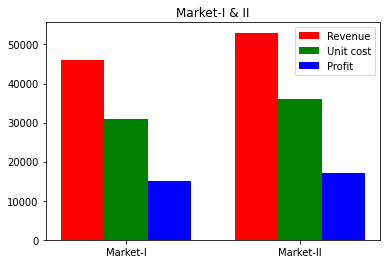
\includegraphics[width=\columnwidth]{solutions/su2021/45/FIGURE.png}
\caption{Revenue,Sales \& Profit Of Market-I \& II}
\label{matrix/2/45/fig:Profit}	
\end{figure}
  \item If A=$\myvec{\alpha &\beta\\ \gamma &-\alpha}$ is such that $A^{2}=I$,then\\
  (A)$1+\alpha^{2}+\beta\gamma=0$ (B)$1-\alpha^{}2+\beta\gamma=0$\\
  (C)$1-\alpha^{2}-\beta\gamma=0$ (D)$1+\alpha^{2}-\beta\gamma=0$\\
\\
\solution
%
\begin{align}
    E(X) &= \frac{1}{\sqrt{2\pi}} \int_{-\infty}^{\infty} x e^{-\frac{x^2}{2}}dx\\
    &=0 \quad \brak{ \text{ odd function}}
\end{align}
\begin{align}
    E\brak{X^2}&= \frac{1}{\sqrt{2\pi}}\int_{-\infty}^{\infty} x^2
e^ {-\frac{x^2}{2}} dx \quad \brak{even function}\\
    &= \frac{2}{\sqrt{2\pi}} \int_{0}^{\infty} x^2 e^{-\frac{x^2}{2}} dx\\
    &= \frac{2}{\sqrt{2\pi}}\int_{0}^{\infty}\sqrt{2u}e^{-u} du \quad\brak{Let \frac{x^2}{2}= u}\\
    &= \frac{2}{\sqrt{\pi}} \int_{0}^{\infty} e^{-u} u^{\frac{3}{2}-1} du\\
    &= \frac{2}{\sqrt{\pi}} \Gamma\brak{{\frac{3}{2}}}\\
    &= \frac{1}{\sqrt{\pi}}\Gamma\brak{\frac{1}{2}} \\
    &= 1
\end{align}
where we have used the fact that
\begin{align}
\quad\because \Gamma(n)= (n-1)\Gamma(n-1); \Gamma\brak{\frac{1}{2}}=\sqrt{\pi}
\end{align}
%
Thus, the  variance is
\begin{align}
    \sigma^2 =  E\brak X^2 - E^2\brak X = 1
\end{align}

  \item If the matrix A is both symmetric and skew symmetric,then\\
  (A) A is a diagonal matrix \\
  (B) A is a zero matriz\\
  (C)A is a square matrix \\
  (D)None of these\\
  \\
\solution
If $\vec{A}$ is symmetric, then 
\begin{align}
\vec{A}^T =\vec{A}
\label{matrix/48/2.0.1}
\end{align}
If matrix A is skew symmetric, then
\begin{align}
\vec{A}^T = \vec{-A}
\label{matrix/48/2.0.2}
\end{align}
From  \eqref{matrix/48/2.0.1} and \eqref{matrix/48/2.0.2},
\begin{align}
\vec{A} &=\vec{-A}
\\
\implies 2\vec{A} &= 0
\\
\text{or, } \vec{A} &= 0
\end{align}
$\therefore $ $\vec{A}$ is zero matrix.


  \item If A is square matrix such that $A^{2}=A$,then $(I+A)^{3}-7A$ is equal to\\
  (A)A \\(B)I-A\\ (C)I\\ (D)3A
\\
\solution
%
\begin{align}
    E(X) &= \frac{1}{\sqrt{2\pi}} \int_{-\infty}^{\infty} x e^{-\frac{x^2}{2}}dx\\
    &=0 \quad \brak{ \text{ odd function}}
\end{align}
\begin{align}
    E\brak{X^2}&= \frac{1}{\sqrt{2\pi}}\int_{-\infty}^{\infty} x^2
e^ {-\frac{x^2}{2}} dx \quad \brak{even function}\\
    &= \frac{2}{\sqrt{2\pi}} \int_{0}^{\infty} x^2 e^{-\frac{x^2}{2}} dx\\
    &= \frac{2}{\sqrt{2\pi}}\int_{0}^{\infty}\sqrt{2u}e^{-u} du \quad\brak{Let \frac{x^2}{2}= u}\\
    &= \frac{2}{\sqrt{\pi}} \int_{0}^{\infty} e^{-u} u^{\frac{3}{2}-1} du\\
    &= \frac{2}{\sqrt{\pi}} \Gamma\brak{{\frac{3}{2}}}\\
    &= \frac{1}{\sqrt{\pi}}\Gamma\brak{\frac{1}{2}} \\
    &= 1
\end{align}
where we have used the fact that
\begin{align}
\quad\because \Gamma(n)= (n-1)\Gamma(n-1); \Gamma\brak{\frac{1}{2}}=\sqrt{\pi}
\end{align}
%
Thus, the  variance is
\begin{align}
    \sigma^2 =  E\brak X^2 - E^2\brak X = 1
\end{align}

\item Balance the following chemical equation.
\begin{align}
  \label{matrix/50/eq1}
NaOH + H_2SO_4 \xrightarrow{} Na_2SO_4  +  H_2O
\end{align}
\\
\solution
Let the balanced version of \eqref{matrix/50/eq1} be
\begin{align}
   x_{1}NaOH + x_{2}H_2SO_4 \xrightarrow{} 
   x_{3}Na_2SO_4 + x_{4}H_2O \label{matrix/50/eq2}
\end{align}
which results in the following equations:
\begin{align}
    (x_{1}-2x_{3}) Na= 0\\
    (x_{1}+4x_{2}-4x_{3}-x_{4}) O= 0\\
    (x_{1}+2x_{2}-2x_{4}) H=0\\
    (x_{2}-x_{3}) S= 0
\end{align}
which can be expressed as
\begin{align}
    x_{1}+ 0.x_{2}- 2x_{3}+ 0.x_{4} = 0\\
    x_{1}+ 4x_{2}- 4x_{3}- x_{4} = 0\\
    x_{1}+ 2x_{2}+ 0.x_{3}- 2x_{4} = 0\\
    0.x_{1}+ x_{2}- x_{3}+ 0.x_{4} = 0
\end{align}
resulting in the matrix equation
\begin{align}
    \myvec{1 & 0 & -2 & 0\\
           1 & 4 & -4 & -1\\
           1 & 2 & 0 & -2\\
           0 & 1 & -1 & 0}\vec{x}
           =\vec{0}    \label{matrix/50/eq3}
\end{align}
where,
\begin{align}
   \vec{x}= \myvec{x_{1}\\x_{2}\\x_{3}\\x_{4}}
\end{align}
\eqref{matrix/50/eq3} can be reduced as follows:
\begin{align}
    \myvec{1 & 0 & -2 & 0\\
           1 & 4 & -4 & -1\\
           1 & 2 & 0 & -2\\
           0 & 1 & -1 & 0}
    \xleftrightarrow[R_{3}\leftarrow R_3-R_{1}]{R_{2}\leftarrow R_2- R_1}
    \myvec{1 & 0 & -2 & 0\\
           0 & 4 & -2 & -1\\
           0 & 2 & 2 & -2\\
           0 & 1 & -1 & 0}\\
    \xleftrightarrow{R_2 \leftarrow \frac{R_2}{4}}
    \myvec{1 & 0 & -2 & 0\\
          0 & 1 & -\frac{1}{2} & -\frac{1}{4}\\
          0 & 2 & 2 & -2\\
          0 & 1 & -1 & 0}\\
    \xleftrightarrow[R_4 \leftarrow R_4 - R_2]{R_3 \leftarrow R_3 - 2R_2}
    \myvec{1 & 0 & -2 & 0\\
           0 & 1 & -\frac{1}{2} & -\frac{1}{4}\\
           0 & 0 & 3 & -\frac{3}{2}\\
           0 & 0 & -\frac{1}{2} & \frac{1}{4}}\\
    \xleftrightarrow{R_3 \leftarrow \frac{R_3}{3}}
    \myvec{1 & 0 & -2 & 0\\
           0 & 1 & -\frac{1}{2} & -\frac{1}{4}\\
           0 & 0 & 1 & -\frac{1}{2}\\
           0 & 0 & -\frac{1}{2} & \frac{1}{4}}\\
    \xleftrightarrow[R_{4}\leftarrow R_4+\frac{R_3}{2}]{R_{2}\leftarrow R_2+ \frac{R_3}{2}}
    \myvec{1 & 0 & -2 & 0\\
           0 & 1 & 0 & -\frac{1}{2}\\
           0 & 0 & 1 & -\frac{1}{2}\\
           0 & 0 & 0 & 0}\\
    \xleftrightarrow{R_1 \leftarrow R_1+2R_3}
    \myvec{1 & 0 & 0 & -1\\
           0 & 1 & 0 & -\frac{1}{2}\\
           0 & 0 & 1 & -\frac{1}{2}\\
           0 & 0 & 0 & 0}
\end{align}
Thus,
\begin{align}
    x_1=x_4, x_2= \frac{1}{2}x_4, x_3=\frac{1}{2}x_4\\
    \implies \quad\vec{x}= x_4\myvec{1\\ \frac{1}{2}\\ \frac{1}{2}\\1} 
\end{align} 
by substituting $x_4= 2$
\begin{align}
    \vec{x}=\myvec{2\\1\\1\\2}
\end{align}
Hence, \eqref{matrix/50/eq2} finally becomes
\hfill\break
%\vspace{5mm}  finally becomes
\begin{align}
    2 NaOH + H_2SO_4 \xrightarrow{} 
    Na_2SO_4 + 2 H_2O
\end{align}
\item     Two farmers Ramkishan and Gurcharan Singh cultivate only three varieties of rice namely Basmati, Permal and Naura. The sale (in Rupees) of these varieties of rice by both the farmers in the month of September and October are given by the following matrices $\vec{A}$ and $\vec{B}$ .

\begin{center}
September Sales(in Rupees)
\end{center}
\begin{align}
    \vec{A}=
    \begin{blockarray}{cccc}
    \text{Basmati} & \text{Permal} & \text{Naura} \\
    \begin{block}{(ccc)(c)}
    10000 & 20000 & 30000 & \text{Ramkishan}\\
    50000 & 30000 & 10000 & \text{Gurucharan} \\
    \end{block}
    \end{blockarray}
\end{align}

\begin{center}
October Sales(in Rupees)
\end{center}
\begin{align}
    \vec{B} =
    \begin{blockarray}{cccc}
    \text{Basmati} & \text{Permal} & \text{Naura} \\
    \begin{block}{(ccc)(c)}
    5000 & 10000 & 6000 & \text{Ramkishan}\\
    20000 & 10000 & 10000 & \text{Gurucharan} \\
    \end{block}
    \end{blockarray}
\end{align}

\begin{enumerate}
    \item Find the combined sales in September and October for each farmer in each variety.
    \item Find the decrease in sales from September to October.
    \item If both farmers receive 2\% profit on gross sales, compute the profit for each farmer and for each variety sold in October.
\end{enumerate}
%
\solution

The given system of inequality can be written in matrix form as
\begin{align}
    \myvec{-1 & -2  \\ -1 & 1 \\ 1 & 1\\ 1 & 0 \\ 0 & 1}\vec{x} \succeq \myvec{-10\\0\\1\\0\\0}
\end{align}
which can be further simplified into 
\begin{align}
    \myvec{-1 & -2 \\ 1 & 0 \\ 0&1}\vec{x} \succeq \myvec{-10\\\frac{-1}{2}\\\frac{-1}{2}}
\end{align}
Let the surplus vector be
\begin{align}
    \vec{u} &= \myvec{u_1\\u_2} \succeq 0
\end{align}
\begin{enumerate}
    \item 
    \begin{align}
        \myvec{-1 & -2 \\ 1 & 0}\vec{x} &\succeq \myvec{-10 \\ \frac{-1}{2}}
        \\
        \implies  \myvec{-1 & -2 \\ 1 & 0}\vec{x} &= \myvec{-10 \\ \frac{-1}{2}} + \vec{u}
    \end{align}
    resulting in 
    \begin{align}
        \vec{x} &= \myvec{-1 & -2 \\ 1 & 0}^{-1}\myvec{-10 \\\frac{-1}{2}} + \myvec{-1 & -2 \\ 1 & 0}^{-1}\vec{u}
        \\
        \implies \vec{x} &= \myvec{\frac{1}{2} \\ \frac{19}{4}} + \myvec{0&1\\ \frac{-1}{2}&\frac{-1}{2}}\vec{u}   \label{ineq/58/eq1}
    \end{align}
    \item 
    \begin{align}
        \myvec{-1& -2 \\ 0 & 1}\vec{x} &\succeq \myvec{-10 \\ \frac{-1}{2}}
        \\
        \implies  \myvec{-1& -2 \\ 0 & 1}\vec{x} &= \myvec{-10 \\ \frac{-1}{2}} + \vec{u}
    \end{align}
    resulting in 
    \begin{align}
        \vec{x} &= \myvec{-1& -2 \\ 0 & 1}^{-1}\myvec{-10 \\ \frac{-1}{2}} + \myvec{-1& -2 \\ 0 & 1}^{-1}\vec{u}
        \\
        \implies \vec{x} &= \myvec{9\\\frac{1}{2}} + \myvec{-1& -2 \\ 0 & 1}\vec{u} \label{ineq/58/eq2}
    \end{align}
\end{enumerate}
Now,solution region which is common to regions of eq. \eqref{ineq/58/eq1} and eq. \eqref{ineq/58/eq2},is given by
\begin{align}
    \boxed{\vec{x} = \myvec{\frac{1}{2}\\\frac{1}{2}}+\myvec{0&1\\\frac{-1}{2}&1}\vec{u}}
\end{align}
%
\begin{figure}[!ht]
\centering
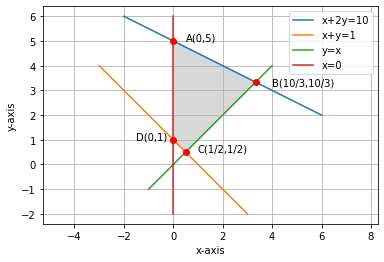
\includegraphics[width=\columnwidth]{solutions/su2021/2/58/Figures/Figure_2.58.png}
\caption{Graphical Solution}
\label{ineq/58/fig:fig1}	
\end{figure}

\begin{figure}[!ht]
\centering
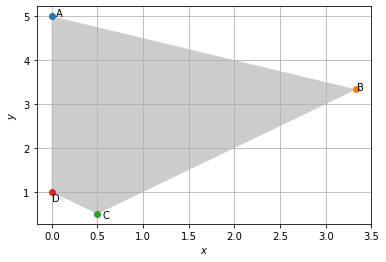
\includegraphics[width=\columnwidth]{solutions/su2021/2/58/Figures/2.58(2).png}
\caption{Magnified Solution region}
\label{ineq/58/fig:fig2}	
\end{figure}


\item If A=$\myvec{1 &2 &3\\3 &-2 &1\\4 &2 &1}$,then show that $A^3-23A-40I=0$
\\  
\solution
Given that $\vec{A}$ =$\myvec{1&2&3\\3&-2&1\\4&2&1}$.
\begin{enumerate}
\item \textbf{The Characteristic equation} is given by:
\begin{align}
  \implies  \abs{\vec{A}-\lambda\vec{I}}&=0
    \\
    \implies \mydet{1-\lambda&2&3\\3&-2-\lambda&1\\4&2&1-\lambda}&=0
    \end{align}
\begin{multline}
   \implies\brak{1-\lambda}\brak{\brak{-2-\lambda}\brak{1-\lambda}-2}
   \\
   -2\brak{3\brak{1-\lambda}-4}+3\brak{6+4\brak{2+\lambda}}=0
\end{multline}
\begin{align}
 \implies   \lambda^3-23\lambda-40=0
\end{align}
The above equation is similar to equation to be proved.
\item According to \textbf{Cayley-Hamilton Theorem:} 
\\
Every square matrix satisfies its own
\\\textbf{characteristic equation}.
\begin{align}
\therefore    \vec{A}^3-23\vec{A}-40\vec{I}=0
\end{align}
Hence Proved.
\end{enumerate}
\item In a legislative assembly election, a political
group hired a public relations firm to promote
its candidate in three ways: telephone, house
calls, and letters. The cost per contact (in paise)
is given in matrix $\vec{A}$ as
\begin{center}
Cost per Contact(in Paise)
\end{center}
\begin{align}
    \vec{A}=
    \begin{blockarray}{cc}
    \text{cost}\\
    \begin{block}{(c)(c)}
    40 &\text{Telephone}\\
    100&\text{Housecall} \\
    50&\text{Letter}\\
    \end{block}
    \end{blockarray}
\end{align}
The number of contacts of each type made in
two cities X and Y is given by matrix $\vec{B}$
\begin{align}
    \vec{B} =
    \begin{blockarray}{cccc}
    \text{Telephone} & \text{Housecall} & \text{Letter} \\
    \begin{block}{(ccc)(c)}
    1000 & 500 & 5000 & \text{X}\\
    3000 & 1000 & 10000 & \text{Y} \\
    \end{block}
    \end{blockarray}
\end{align}
Find the total
amount spent by the group in the two cities
X and Y
%
\solution

The total amount spent is given by=

    \begin{multline}
    \vec{B}\vec{A}\\
    =\myvec{1000&500&5000\\3000&1000&10000}\myvec{40\\100\\50}\\
    =\myvec{40000+50000+250000\\120000+100000+500000}\\
    \begin{blockarray}{cc}
    \text{TotalCost} \\
    \begin{block}{(c)(c)}
    340000&\text{X}\\
    720000&\text{Y}\\
    \end{block}
    \end{blockarray}
    \end{multline}
$\therefore$ the total amount spent in city X and city Y is 3400 and 7200 Rupees respectively.  See Fig. \ref{matrix/64fig:Profit}	
%
\begin{figure}[!ht]
\centering
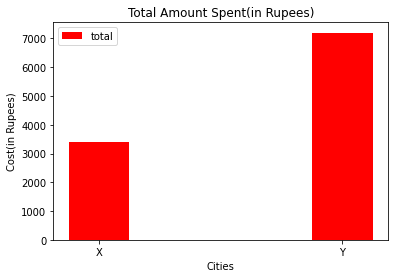
\includegraphics[width=\columnwidth]{solutions/su2021/64/figure8.png}
\caption{Total Amount Spent by the group in cities X and Y}
\label{matrix/64fig:Profit}	
\end{figure}

\item Express the matrix B=$\myvec{2 &-2 &-4\\-1 &3 &4\\1 &-2 &-3}$ as the sum of a symmetric and a skew symmetric matrix.\\
\solution
  We obtain the vertices of the rhombus as follows
\begin{align}
\vec{A} = \myvec{-3\\0},
\vec{B} = \myvec{0\\-3.5},
\vec{C} = \myvec{3\\0},
\vec{D} = \myvec{0\\3.5}
\end{align}
which are plotted in Fig. \ref{quad/45/fig:Rhombus ABCD}.
%
\begin{figure}[ht!]
\centering
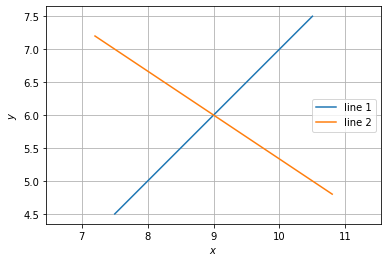
\includegraphics[width=\columnwidth]{solutions/quad/45/figure2.png}
\caption{Rhombus ABCD}
\label{quad/45/fig:Rhombus ABCD}
\end{figure}

  \item Obtain the inverse of the following matrix using elementary operations\\
  A=$\myvec{0 &1 &2\\1 &2 &3\\3 &1 &1}$.\\
  \solution
    \begin{enumerate}
    \item Given that
    \begin{align}
    \vec{A}& =\myvec {0 & 1 & 2\\1 & 2 & 3\\3 & 1 & 1}
    \end{align}
     The augmented matrix $[A | I]$ is as given below:- 
    \begin{align}
    \myvec{0 & 1 & 2 & \vrule & 1 & 0 & 0\\1 & 2 & 3 & \vrule & 0 & 1 & 0\\3 & 1 & 1 & \vrule & 0 & 0 & 1}
    \end{align}
    We apply the elementary row operations on $[A | I]$ as follows :-
    \begin{align}
    [A | I] = \myvec{0 & 1 & 2 & \vrule & 1 & 0 & 0\\1 & 2 & 3 & \vrule & 0 & 1 & 0\\3 & 1 & 1 & \vrule & 0 & 0 & 1}
    \\
    \xleftrightarrow{R_1\leftrightarrow R_2}   
    \myvec{1 & 2 & 3 & \vrule & 0 & 1 & 0\\0 & 1 & 2 & \vrule & 1 & 0 & 0\\3 & 1 & 1 & \vrule & 0 & 0 & 1}
    \\
    \xleftrightarrow{R_3\leftarrow R_3-3R_1}   
    \myvec{1 & 2 & 3 & \vrule & 0 & 1 & 0\\0 & 1 & 2 & \vrule & 1 & 0 & 0\\0 & -5 & -8 & \vrule & 0 & -3 & 1}
    \\
    \xleftrightarrow{R_1\leftarrow R_1-2R_2}  
    \myvec{1 & 0 & -1 & \vrule & -2 & 1 & 0\\0 & 1 & 2 & \vrule & 1 & 0 & 0\\0 & -5 & -8 & \vrule & 0 & -3 & 1}
    \\
    \xleftrightarrow{R_3\leftarrow R_3+5R_2}  
    \myvec{1 & 0 & -1 & \vrule & -2 & 1 & 0\\0 & 1 & 2 & \vrule & 1 & 0 & 0\\0 & 0 & 2 & \vrule & 5 & -3 & 1}
    \\
    \xleftrightarrow{R_3\leftarrow R_3/2}
    \myvec{1 & 0 & -1 & \vrule & -2 & 1 & 0\\ 0 & 1 & 2 & \vrule & 1 & 0 & 0\\0 & 0 & 1 &\vrule &\frac{5}{2} &\frac{-3}{2} &\frac{1}{2}}
    \\
    \xleftrightarrow{R_1\leftarrow R_1+R_3}
    \myvec{1 & 0 & 0 & \vrule & \frac{1}{2} & \frac{-1}{2} & \frac{1}{2}\\ 0 & 1 & 2 & \vrule & 1 & 0 & 0\\0 & 0 & 1 &\vrule &\frac{5}{2} &\frac{-3}{2} &\frac{1}{2}}
    \\
    \xleftrightarrow{R_2\leftarrow R_2-2R_3}
    \myvec{1 & 0 & 0 & \vrule & \frac{1}{2} & \frac{-1}{2} & \frac{1}{2}\\ 0 & 1 & 0 & \vrule & -4 & 3 & -1\\0 & 0 & 1 &\vrule &\frac{5}{2} &\frac{-3}{2} &\frac{1}{2}}
    \end{align}
    By performing elementary transformations on augmented matrix$ [A | I]$ , we obtained the augmented matrix in the form $ [I | A]$. 
    Hence we can conclude that the matrix A is invertible and inverse of the matrix is:-
    \begin{align}
    \therefore\vec{A^{-1}}=\myvec { \frac{1}{2} & \frac{-1}{2} & \frac{1}{2} \\  -4 & 3 & -1\\ \frac{5}{2} &\frac{-3}{2} &\frac{1}{2}}
    \end{align}
    \item QR decomposition of  \myvec{0  & 1 & 3 \\ 1 & 2 & 3 \\ 2 & 3 & 1}
    \\
     Let us use the Gram-schmidt approach to obtain QR decomposition of$ \vec{A}$. Consider rows vectors say $\vec{a_1}$,$\vec{a_2}$ and $\vec{a_3}$ of $\vec{A}$  which is given by
    \begin{align}
    \vec{a_1}=\myvec{0 & 1 & 2}\label{matrix/69/eq1}\\
    \vec{a_2}=\myvec{1 & 2 & 3}\label{matrix/69/eq2}\\
    \vec{a_3}=\myvec{3 & 1 & 1}\label{matrix/69/eq3}
    \end{align}
    we can express these as 
    \begin{align}
    \vec{u_1}&=\vec{a_1}=\myvec{0 & 1 & 2}\label{matrix/69/eq4}\\
    \vec{e_1}&=\frac{\vec{u_1}}{\norm{\vec{u_1}}}\\
    \vec{e_1}&=\frac{\myvec{0 & 1 & 2}}{\sqrt{0+1+4}}\\
    \vec{e_1}&=\myvec{0 & \frac{1}{\sqrt{5}} & \frac{2}{\sqrt{5}}}\\
    \vec{u_2}&=\vec{a_2}-(\vec{a_2}\vec{e_1})\vec{e_1}\\
    &=\myvec{1 & 2 & 3}-(\myvec{1 & 2 & 3}\myvec{0 & \frac{1}{\sqrt{5}} & \frac{2}{\sqrt{5}}})\myvec{0 & \frac{1}{\sqrt{5}} &  \frac{2}{\sqrt{5}}}\\
    &=\myvec{1 & \frac{2}{5} & \frac{-1}{5}}\\
    \vec{e_2}&=\frac{\vec{u_2}}{\norm{\vec{u_2}}}=\frac{\myvec{1 & \frac{2}{5} & \frac{-1}{5}}}{\sqrt{1+\frac{4}{25}+\frac{1}{25}}}\\
    \vec{e_2}&=\myvec{\frac{5}{\sqrt{30}} & \frac{2}{\sqrt{30}} &\frac{-1}{\sqrt{30}}}\\
    \vec{u_3}&=\vec{a_3}-(\vec{a_3}\vec{e_1})\vec{e_1}-(\vec{a_3}\vec{e_2})\vec{e_2}
    \\
    \vec{u_3}&=\myvec{\frac{1}{3} & \frac{-2}{3} &\frac{1}{3}}\\
    \vec{e_3}&=\frac{\vec{u_3}}{\norm{\vec{u_3}}}\\
    &=\frac{\myvec{\frac{1}{3} & \frac{-2}{3} & \frac{1}{4}}}{\sqrt{\frac{1}{9}+\frac{4}{9}+\frac{1}{9}}}\\
    \vec{e_3}&=\myvec{\frac{1}{\sqrt{6}} & \frac{-2}{\sqrt{6}} &\frac{1}{\sqrt{6}}}
    \end{align}
    Thus,
    \begin{align}
     \vec{Q}&=(e_1|e_2|----|e_n)\\
     &=\myvec{0 & \frac{5}{\sqrt{30}} & \frac{1}{\sqrt{6}}\\\frac{1}{\sqrt{5}} & \frac{2}{\sqrt{30}} & \frac{-2}{\sqrt{6}}\\\frac{2}{\sqrt{5}} & \frac{-1}{\sqrt{30}} & \frac{1}{\sqrt{6}}}\label{matrix/69/eq5}      
    \end{align}
    Then
    \begin{align}
      \vec{R}&=\myvec{a_1e_1 & a_2e_1 & a_3e_1\\ 0 & a_2e_2 & a_3e_2\\0 & 0 & a_3e_3}\\
      &=\myvec{\frac{5}{\sqrt{5}} & \frac{8}{\sqrt{5}} & \frac{3}{\sqrt{5}}\\0 &  \frac{6}{\sqrt{30}} & \frac{16}{\sqrt{30}}\\0 & 0 & \frac{2}{\sqrt{6}}}\label{matrix/69/eq6} 
      \end{align}
    From equations \eqref{matrix/69/eq5} and \eqref{matrix/69/eq6} the obtained $\vec{Q} \vec{R}$ Decomposition is
    \begin{align}
     \myvec{0  & 1 & 3 \\ 1 & 2 & 3 \\ 2 & 3 & 1}&= \myvec{0 & \frac{5}{\sqrt{30}} & \frac{1}{\sqrt{6}}\\\frac{1}{\sqrt{5}} & \frac{2}{\sqrt{30}} & \frac{-2}{\sqrt{6}}\\\frac{2}{\sqrt{5}} & \frac{-1}{\sqrt{30}} & \frac{1}{\sqrt{6}}}\myvec{\frac{5}{\sqrt{5}} & \frac{8}{\sqrt{5}} & \frac{3}{\sqrt{5}}\\0 &  \frac{6}{\sqrt{30}} & \frac{16}{\sqrt{30}}\\0 & 0 & \frac{2}{\sqrt{6}}} 
    \end{align}
    \end{enumerate}
    \item Find P$^{-1}$, if it exists, given \\
    P=$\myvec{10 &-2\\-5 &1}$.\\
    \solution
    Using row reduction, 
%
\begin{align}
\myvec{10 & -2 \\-5 & 1}
\xleftrightarrow {R_2 \leftarrow R_2+\frac{R_1}{2}}\myvec{10& -2& \\0 & 0}
\end{align} 
Hence,  $\vec {P}^{-1} $ does not exist.
     
%\end{enumerate}
%\end{document}
    

%\renewcommand{\theequation}{\theenumi}
%\begin{enumerate}[label=\arabic*.,ref=\thesubsection.\theenumi]
%\numberwithin{equation}{enumi}

\item Find 
$\begin{vmatrix}
2&4\\-5&-1
\end{vmatrix}$
\\
\solution 
%
\begin{align}
    E(X) &= \frac{1}{\sqrt{2\pi}} \int_{-\infty}^{\infty} x e^{-\frac{x^2}{2}}dx\\
    &=0 \quad \brak{ \text{ odd function}}
\end{align}
\begin{align}
    E\brak{X^2}&= \frac{1}{\sqrt{2\pi}}\int_{-\infty}^{\infty} x^2
e^ {-\frac{x^2}{2}} dx \quad \brak{even function}\\
    &= \frac{2}{\sqrt{2\pi}} \int_{0}^{\infty} x^2 e^{-\frac{x^2}{2}} dx\\
    &= \frac{2}{\sqrt{2\pi}}\int_{0}^{\infty}\sqrt{2u}e^{-u} du \quad\brak{Let \frac{x^2}{2}= u}\\
    &= \frac{2}{\sqrt{\pi}} \int_{0}^{\infty} e^{-u} u^{\frac{3}{2}-1} du\\
    &= \frac{2}{\sqrt{\pi}} \Gamma\brak{{\frac{3}{2}}}\\
    &= \frac{1}{\sqrt{\pi}}\Gamma\brak{\frac{1}{2}} \\
    &= 1
\end{align}
where we have used the fact that
\begin{align}
\quad\because \Gamma(n)= (n-1)\Gamma(n-1); \Gamma\brak{\frac{1}{2}}=\sqrt{\pi}
\end{align}
%
Thus, the  variance is
\begin{align}
    \sigma^2 =  E\brak X^2 - E^2\brak X = 1
\end{align}


\item (i) $\begin{vmatrix}\cos\theta& -\sin\theta\\ \sin\theta& \cos\theta \end{vmatrix}$ 
(ii) $\begin{vmatrix}
x^2-x+1& x-1\\ x+1&  x+1
\end{vmatrix}$
\\
\solution 
%
\begin{align}
    E(X) &= \frac{1}{\sqrt{2\pi}} \int_{-\infty}^{\infty} x e^{-\frac{x^2}{2}}dx\\
    &=0 \quad \brak{ \text{ odd function}}
\end{align}
\begin{align}
    E\brak{X^2}&= \frac{1}{\sqrt{2\pi}}\int_{-\infty}^{\infty} x^2
e^ {-\frac{x^2}{2}} dx \quad \brak{even function}\\
    &= \frac{2}{\sqrt{2\pi}} \int_{0}^{\infty} x^2 e^{-\frac{x^2}{2}} dx\\
    &= \frac{2}{\sqrt{2\pi}}\int_{0}^{\infty}\sqrt{2u}e^{-u} du \quad\brak{Let \frac{x^2}{2}= u}\\
    &= \frac{2}{\sqrt{\pi}} \int_{0}^{\infty} e^{-u} u^{\frac{3}{2}-1} du\\
    &= \frac{2}{\sqrt{\pi}} \Gamma\brak{{\frac{3}{2}}}\\
    &= \frac{1}{\sqrt{\pi}}\Gamma\brak{\frac{1}{2}} \\
    &= 1
\end{align}
where we have used the fact that
\begin{align}
\quad\because \Gamma(n)= (n-1)\Gamma(n-1); \Gamma\brak{\frac{1}{2}}=\sqrt{\pi}
\end{align}
%
Thus, the  variance is
\begin{align}
    \sigma^2 =  E\brak X^2 - E^2\brak X = 1
\end{align}

\item If$ \vec{A} = \begin{vmatrix}1&2\\4&2\end{vmatrix}$,then show that  
$\abs{2\vec{A}}=4\abs{\vec{A}}$
\\
\solution 
%
\begin{align}
    E(X) &= \frac{1}{\sqrt{2\pi}} \int_{-\infty}^{\infty} x e^{-\frac{x^2}{2}}dx\\
    &=0 \quad \brak{ \text{ odd function}}
\end{align}
\begin{align}
    E\brak{X^2}&= \frac{1}{\sqrt{2\pi}}\int_{-\infty}^{\infty} x^2
e^ {-\frac{x^2}{2}} dx \quad \brak{even function}\\
    &= \frac{2}{\sqrt{2\pi}} \int_{0}^{\infty} x^2 e^{-\frac{x^2}{2}} dx\\
    &= \frac{2}{\sqrt{2\pi}}\int_{0}^{\infty}\sqrt{2u}e^{-u} du \quad\brak{Let \frac{x^2}{2}= u}\\
    &= \frac{2}{\sqrt{\pi}} \int_{0}^{\infty} e^{-u} u^{\frac{3}{2}-1} du\\
    &= \frac{2}{\sqrt{\pi}} \Gamma\brak{{\frac{3}{2}}}\\
    &= \frac{1}{\sqrt{\pi}}\Gamma\brak{\frac{1}{2}} \\
    &= 1
\end{align}
where we have used the fact that
\begin{align}
\quad\because \Gamma(n)= (n-1)\Gamma(n-1); \Gamma\brak{\frac{1}{2}}=\sqrt{\pi}
\end{align}
%
Thus, the  variance is
\begin{align}
    \sigma^2 =  E\brak X^2 - E^2\brak X = 1
\end{align}

\item If $\vec{A}=\begin{vmatrix}1&0&1\\0&1&2\\0&0&4\end{vmatrix}$, then show that $\abs{3\vec{A}}=27\abs{\vec{A}}$
\\
\solution 
%
\begin{align}
    E(X) &= \frac{1}{\sqrt{2\pi}} \int_{-\infty}^{\infty} x e^{-\frac{x^2}{2}}dx\\
    &=0 \quad \brak{ \text{ odd function}}
\end{align}
\begin{align}
    E\brak{X^2}&= \frac{1}{\sqrt{2\pi}}\int_{-\infty}^{\infty} x^2
e^ {-\frac{x^2}{2}} dx \quad \brak{even function}\\
    &= \frac{2}{\sqrt{2\pi}} \int_{0}^{\infty} x^2 e^{-\frac{x^2}{2}} dx\\
    &= \frac{2}{\sqrt{2\pi}}\int_{0}^{\infty}\sqrt{2u}e^{-u} du \quad\brak{Let \frac{x^2}{2}= u}\\
    &= \frac{2}{\sqrt{\pi}} \int_{0}^{\infty} e^{-u} u^{\frac{3}{2}-1} du\\
    &= \frac{2}{\sqrt{\pi}} \Gamma\brak{{\frac{3}{2}}}\\
    &= \frac{1}{\sqrt{\pi}}\Gamma\brak{\frac{1}{2}} \\
    &= 1
\end{align}
where we have used the fact that
\begin{align}
\quad\because \Gamma(n)= (n-1)\Gamma(n-1); \Gamma\brak{\frac{1}{2}}=\sqrt{\pi}
\end{align}
%
Thus, the  variance is
\begin{align}
    \sigma^2 =  E\brak X^2 - E^2\brak X = 1
\end{align}

\item Evaluate the determinants
\begin{enumerate}
\item $\begin{vmatrix}
3&-1&-2\\0&0&-1\\3&-5&0
\end{vmatrix}$
\item $\begin{vmatrix}
3&-4&5\\1&1&-2\\2&3&1
\end{vmatrix}$
\\
\solution 
\input{./solutions/5/chapters/lines/docq14.tex}
\item $\begin{vmatrix}
0&1&2 \\ -1&0&-3\\-2&3&0
\end{vmatrix}$
\item $\begin{vmatrix}
2&-1&-2\\0&2&-1\\3&-5&0
\end{vmatrix}$
\end{enumerate}  
\item If A=$\begin{vmatrix}1&1&-2\\2&1&-3\\5&4&-9\end{vmatrix}$, 
find $\abs{A}$
\\
\solution 
%
\begin{align}
    E(X) &= \frac{1}{\sqrt{2\pi}} \int_{-\infty}^{\infty} x e^{-\frac{x^2}{2}}dx\\
    &=0 \quad \brak{ \text{ odd function}}
\end{align}
\begin{align}
    E\brak{X^2}&= \frac{1}{\sqrt{2\pi}}\int_{-\infty}^{\infty} x^2
e^ {-\frac{x^2}{2}} dx \quad \brak{even function}\\
    &= \frac{2}{\sqrt{2\pi}} \int_{0}^{\infty} x^2 e^{-\frac{x^2}{2}} dx\\
    &= \frac{2}{\sqrt{2\pi}}\int_{0}^{\infty}\sqrt{2u}e^{-u} du \quad\brak{Let \frac{x^2}{2}= u}\\
    &= \frac{2}{\sqrt{\pi}} \int_{0}^{\infty} e^{-u} u^{\frac{3}{2}-1} du\\
    &= \frac{2}{\sqrt{\pi}} \Gamma\brak{{\frac{3}{2}}}\\
    &= \frac{1}{\sqrt{\pi}}\Gamma\brak{\frac{1}{2}} \\
    &= 1
\end{align}
where we have used the fact that
\begin{align}
\quad\because \Gamma(n)= (n-1)\Gamma(n-1); \Gamma\brak{\frac{1}{2}}=\sqrt{\pi}
\end{align}
%
Thus, the  variance is
\begin{align}
    \sigma^2 =  E\brak X^2 - E^2\brak X = 1
\end{align}

\item Find the values of x,If\\
(i)$\begin{vmatrix}
2&4\\5&1
\end{vmatrix}$ =$\begin{vmatrix}
2x&4 \\ 6&x
\end{vmatrix}$
(ii)$\begin{vmatrix}
2&3 \\ 4&5
\end{vmatrix}$ =$\begin{vmatrix}
x&3 \\ 2x&5
\end{vmatrix}$
\\
\solution 
%
\begin{align}
    E(X) &= \frac{1}{\sqrt{2\pi}} \int_{-\infty}^{\infty} x e^{-\frac{x^2}{2}}dx\\
    &=0 \quad \brak{ \text{ odd function}}
\end{align}
\begin{align}
    E\brak{X^2}&= \frac{1}{\sqrt{2\pi}}\int_{-\infty}^{\infty} x^2
e^ {-\frac{x^2}{2}} dx \quad \brak{even function}\\
    &= \frac{2}{\sqrt{2\pi}} \int_{0}^{\infty} x^2 e^{-\frac{x^2}{2}} dx\\
    &= \frac{2}{\sqrt{2\pi}}\int_{0}^{\infty}\sqrt{2u}e^{-u} du \quad\brak{Let \frac{x^2}{2}= u}\\
    &= \frac{2}{\sqrt{\pi}} \int_{0}^{\infty} e^{-u} u^{\frac{3}{2}-1} du\\
    &= \frac{2}{\sqrt{\pi}} \Gamma\brak{{\frac{3}{2}}}\\
    &= \frac{1}{\sqrt{\pi}}\Gamma\brak{\frac{1}{2}} \\
    &= 1
\end{align}
where we have used the fact that
\begin{align}
\quad\because \Gamma(n)= (n-1)\Gamma(n-1); \Gamma\brak{\frac{1}{2}}=\sqrt{\pi}
\end{align}
%
Thus, the  variance is
\begin{align}
    \sigma^2 =  E\brak X^2 - E^2\brak X = 1
\end{align}

\item If  $\begin{vmatrix}
x&2 \\ 18&x
\end{vmatrix}$ =$\begin{vmatrix}
6&2 \\ 18&6
\end{vmatrix}$, then x is equal to 
\begin{enumerate}
\item 6
\item $\pm 6$
\item $-6$
\item 0
\end{enumerate}
\item $\begin{vmatrix}
x&a&x+a\\y&b&y+b\\z&c&z+c\end{vmatrix}=0$
\\
\solution 
%
\begin{align}
    E(X) &= \frac{1}{\sqrt{2\pi}} \int_{-\infty}^{\infty} x e^{-\frac{x^2}{2}}dx\\
    &=0 \quad \brak{ \text{ odd function}}
\end{align}
\begin{align}
    E\brak{X^2}&= \frac{1}{\sqrt{2\pi}}\int_{-\infty}^{\infty} x^2
e^ {-\frac{x^2}{2}} dx \quad \brak{even function}\\
    &= \frac{2}{\sqrt{2\pi}} \int_{0}^{\infty} x^2 e^{-\frac{x^2}{2}} dx\\
    &= \frac{2}{\sqrt{2\pi}}\int_{0}^{\infty}\sqrt{2u}e^{-u} du \quad\brak{Let \frac{x^2}{2}= u}\\
    &= \frac{2}{\sqrt{\pi}} \int_{0}^{\infty} e^{-u} u^{\frac{3}{2}-1} du\\
    &= \frac{2}{\sqrt{\pi}} \Gamma\brak{{\frac{3}{2}}}\\
    &= \frac{1}{\sqrt{\pi}}\Gamma\brak{\frac{1}{2}} \\
    &= 1
\end{align}
where we have used the fact that
\begin{align}
\quad\because \Gamma(n)= (n-1)\Gamma(n-1); \Gamma\brak{\frac{1}{2}}=\sqrt{\pi}
\end{align}
%
Thus, the  variance is
\begin{align}
    \sigma^2 =  E\brak X^2 - E^2\brak X = 1
\end{align}

\item $\begin{vmatrix}
a-b&b-c&c-a\\b-c&c-a&a-b\\c-a&a-b&b-c\end{vmatrix}=0$
\\
\solution 
%
\begin{align}
    E(X) &= \frac{1}{\sqrt{2\pi}} \int_{-\infty}^{\infty} x e^{-\frac{x^2}{2}}dx\\
    &=0 \quad \brak{ \text{ odd function}}
\end{align}
\begin{align}
    E\brak{X^2}&= \frac{1}{\sqrt{2\pi}}\int_{-\infty}^{\infty} x^2
e^ {-\frac{x^2}{2}} dx \quad \brak{even function}\\
    &= \frac{2}{\sqrt{2\pi}} \int_{0}^{\infty} x^2 e^{-\frac{x^2}{2}} dx\\
    &= \frac{2}{\sqrt{2\pi}}\int_{0}^{\infty}\sqrt{2u}e^{-u} du \quad\brak{Let \frac{x^2}{2}= u}\\
    &= \frac{2}{\sqrt{\pi}} \int_{0}^{\infty} e^{-u} u^{\frac{3}{2}-1} du\\
    &= \frac{2}{\sqrt{\pi}} \Gamma\brak{{\frac{3}{2}}}\\
    &= \frac{1}{\sqrt{\pi}}\Gamma\brak{\frac{1}{2}} \\
    &= 1
\end{align}
where we have used the fact that
\begin{align}
\quad\because \Gamma(n)= (n-1)\Gamma(n-1); \Gamma\brak{\frac{1}{2}}=\sqrt{\pi}
\end{align}
%
Thus, the  variance is
\begin{align}
    \sigma^2 =  E\brak X^2 - E^2\brak X = 1
\end{align}

\item $\begin{vmatrix}2&7&65\\3&8&75\\5&9&86\end{vmatrix}=0$
\\
\solution 
%
\begin{align}
    E(X) &= \frac{1}{\sqrt{2\pi}} \int_{-\infty}^{\infty} x e^{-\frac{x^2}{2}}dx\\
    &=0 \quad \brak{ \text{ odd function}}
\end{align}
\begin{align}
    E\brak{X^2}&= \frac{1}{\sqrt{2\pi}}\int_{-\infty}^{\infty} x^2
e^ {-\frac{x^2}{2}} dx \quad \brak{even function}\\
    &= \frac{2}{\sqrt{2\pi}} \int_{0}^{\infty} x^2 e^{-\frac{x^2}{2}} dx\\
    &= \frac{2}{\sqrt{2\pi}}\int_{0}^{\infty}\sqrt{2u}e^{-u} du \quad\brak{Let \frac{x^2}{2}= u}\\
    &= \frac{2}{\sqrt{\pi}} \int_{0}^{\infty} e^{-u} u^{\frac{3}{2}-1} du\\
    &= \frac{2}{\sqrt{\pi}} \Gamma\brak{{\frac{3}{2}}}\\
    &= \frac{1}{\sqrt{\pi}}\Gamma\brak{\frac{1}{2}} \\
    &= 1
\end{align}
where we have used the fact that
\begin{align}
\quad\because \Gamma(n)= (n-1)\Gamma(n-1); \Gamma\brak{\frac{1}{2}}=\sqrt{\pi}
\end{align}
%
Thus, the  variance is
\begin{align}
    \sigma^2 =  E\brak X^2 - E^2\brak X = 1
\end{align}

\item $\begin{vmatrix}1&bc&a(b+c)\\1&ca&b(c+a)\\1&ab&c(a+b)\end{vmatrix}=0$
\\
\solution 
%
\begin{align}
    E(X) &= \frac{1}{\sqrt{2\pi}} \int_{-\infty}^{\infty} x e^{-\frac{x^2}{2}}dx\\
    &=0 \quad \brak{ \text{ odd function}}
\end{align}
\begin{align}
    E\brak{X^2}&= \frac{1}{\sqrt{2\pi}}\int_{-\infty}^{\infty} x^2
e^ {-\frac{x^2}{2}} dx \quad \brak{even function}\\
    &= \frac{2}{\sqrt{2\pi}} \int_{0}^{\infty} x^2 e^{-\frac{x^2}{2}} dx\\
    &= \frac{2}{\sqrt{2\pi}}\int_{0}^{\infty}\sqrt{2u}e^{-u} du \quad\brak{Let \frac{x^2}{2}= u}\\
    &= \frac{2}{\sqrt{\pi}} \int_{0}^{\infty} e^{-u} u^{\frac{3}{2}-1} du\\
    &= \frac{2}{\sqrt{\pi}} \Gamma\brak{{\frac{3}{2}}}\\
    &= \frac{1}{\sqrt{\pi}}\Gamma\brak{\frac{1}{2}} \\
    &= 1
\end{align}
where we have used the fact that
\begin{align}
\quad\because \Gamma(n)= (n-1)\Gamma(n-1); \Gamma\brak{\frac{1}{2}}=\sqrt{\pi}
\end{align}
%
Thus, the  variance is
\begin{align}
    \sigma^2 =  E\brak X^2 - E^2\brak X = 1
\end{align}

\item $\begin{vmatrix}b+c& q+r& y+z\\c+a& r+p& z+x\\a+b& p+q& x+y\end{vmatrix}$=2$\begin{vmatrix} a&p&x\\b&q&y\\c&r&z\end{vmatrix}$ 
\\
\solution 
%
\begin{align}
    E(X) &= \frac{1}{\sqrt{2\pi}} \int_{-\infty}^{\infty} x e^{-\frac{x^2}{2}}dx\\
    &=0 \quad \brak{ \text{ odd function}}
\end{align}
\begin{align}
    E\brak{X^2}&= \frac{1}{\sqrt{2\pi}}\int_{-\infty}^{\infty} x^2
e^ {-\frac{x^2}{2}} dx \quad \brak{even function}\\
    &= \frac{2}{\sqrt{2\pi}} \int_{0}^{\infty} x^2 e^{-\frac{x^2}{2}} dx\\
    &= \frac{2}{\sqrt{2\pi}}\int_{0}^{\infty}\sqrt{2u}e^{-u} du \quad\brak{Let \frac{x^2}{2}= u}\\
    &= \frac{2}{\sqrt{\pi}} \int_{0}^{\infty} e^{-u} u^{\frac{3}{2}-1} du\\
    &= \frac{2}{\sqrt{\pi}} \Gamma\brak{{\frac{3}{2}}}\\
    &= \frac{1}{\sqrt{\pi}}\Gamma\brak{\frac{1}{2}} \\
    &= 1
\end{align}
where we have used the fact that
\begin{align}
\quad\because \Gamma(n)= (n-1)\Gamma(n-1); \Gamma\brak{\frac{1}{2}}=\sqrt{\pi}
\end{align}
%
Thus, the  variance is
\begin{align}
    \sigma^2 =  E\brak X^2 - E^2\brak X = 1
\end{align}

\item $\begin{vmatrix}-a^2&ab&ab\\ ba&-b^2&bc\\ ca&cb&-c^2\end{vmatrix}$=$4a^2b^2c^2$\\
\\
\solution 
%
\begin{align}
    E(X) &= \frac{1}{\sqrt{2\pi}} \int_{-\infty}^{\infty} x e^{-\frac{x^2}{2}}dx\\
    &=0 \quad \brak{ \text{ odd function}}
\end{align}
\begin{align}
    E\brak{X^2}&= \frac{1}{\sqrt{2\pi}}\int_{-\infty}^{\infty} x^2
e^ {-\frac{x^2}{2}} dx \quad \brak{even function}\\
    &= \frac{2}{\sqrt{2\pi}} \int_{0}^{\infty} x^2 e^{-\frac{x^2}{2}} dx\\
    &= \frac{2}{\sqrt{2\pi}}\int_{0}^{\infty}\sqrt{2u}e^{-u} du \quad\brak{Let \frac{x^2}{2}= u}\\
    &= \frac{2}{\sqrt{\pi}} \int_{0}^{\infty} e^{-u} u^{\frac{3}{2}-1} du\\
    &= \frac{2}{\sqrt{\pi}} \Gamma\brak{{\frac{3}{2}}}\\
    &= \frac{1}{\sqrt{\pi}}\Gamma\brak{\frac{1}{2}} \\
    &= 1
\end{align}
where we have used the fact that
\begin{align}
\quad\because \Gamma(n)= (n-1)\Gamma(n-1); \Gamma\brak{\frac{1}{2}}=\sqrt{\pi}
\end{align}
%
Thus, the  variance is
\begin{align}
    \sigma^2 =  E\brak X^2 - E^2\brak X = 1
\end{align}

By Using properties of determinants, in Exercises 16 to 22,Show that;
\item (i)$\begin{vmatrix}1&a&a^2\\1&b&b^2\\1&c&c^2\end{vmatrix}$=(a-b)(b-c)(c-a)\\
(ii) $\begin{vmatrix}1&1&1 \\ a&b&c \\ a^3&b^3&c^3\end{vmatrix}$=(a-b)(b-c)(c-a)(a+b+c)
\\
\solution 
%
\begin{align}
    E(X) &= \frac{1}{\sqrt{2\pi}} \int_{-\infty}^{\infty} x e^{-\frac{x^2}{2}}dx\\
    &=0 \quad \brak{ \text{ odd function}}
\end{align}
\begin{align}
    E\brak{X^2}&= \frac{1}{\sqrt{2\pi}}\int_{-\infty}^{\infty} x^2
e^ {-\frac{x^2}{2}} dx \quad \brak{even function}\\
    &= \frac{2}{\sqrt{2\pi}} \int_{0}^{\infty} x^2 e^{-\frac{x^2}{2}} dx\\
    &= \frac{2}{\sqrt{2\pi}}\int_{0}^{\infty}\sqrt{2u}e^{-u} du \quad\brak{Let \frac{x^2}{2}= u}\\
    &= \frac{2}{\sqrt{\pi}} \int_{0}^{\infty} e^{-u} u^{\frac{3}{2}-1} du\\
    &= \frac{2}{\sqrt{\pi}} \Gamma\brak{{\frac{3}{2}}}\\
    &= \frac{1}{\sqrt{\pi}}\Gamma\brak{\frac{1}{2}} \\
    &= 1
\end{align}
where we have used the fact that
\begin{align}
\quad\because \Gamma(n)= (n-1)\Gamma(n-1); \Gamma\brak{\frac{1}{2}}=\sqrt{\pi}
\end{align}
%
Thus, the  variance is
\begin{align}
    \sigma^2 =  E\brak X^2 - E^2\brak X = 1
\end{align}

\item $\begin{vmatrix}x&x^2&yz \\ y&y^2&zx \\ z&z^2&xy\end{vmatrix}$=(x-y)(y-z)(z-x)(xy+yz+zx)
\item (i) $\begin{vmatrix}x+4&2x&2x \\ 2x&x+4&2x \\ 2x&2x&x+4\end{vmatrix}$=$(5x+4)(4-x)^2$\\
\solution 
%
\begin{align}
    E(X) &= \frac{1}{\sqrt{2\pi}} \int_{-\infty}^{\infty} x e^{-\frac{x^2}{2}}dx\\
    &=0 \quad \brak{ \text{ odd function}}
\end{align}
\begin{align}
    E\brak{X^2}&= \frac{1}{\sqrt{2\pi}}\int_{-\infty}^{\infty} x^2
e^ {-\frac{x^2}{2}} dx \quad \brak{even function}\\
    &= \frac{2}{\sqrt{2\pi}} \int_{0}^{\infty} x^2 e^{-\frac{x^2}{2}} dx\\
    &= \frac{2}{\sqrt{2\pi}}\int_{0}^{\infty}\sqrt{2u}e^{-u} du \quad\brak{Let \frac{x^2}{2}= u}\\
    &= \frac{2}{\sqrt{\pi}} \int_{0}^{\infty} e^{-u} u^{\frac{3}{2}-1} du\\
    &= \frac{2}{\sqrt{\pi}} \Gamma\brak{{\frac{3}{2}}}\\
    &= \frac{1}{\sqrt{\pi}}\Gamma\brak{\frac{1}{2}} \\
    &= 1
\end{align}
where we have used the fact that
\begin{align}
\quad\because \Gamma(n)= (n-1)\Gamma(n-1); \Gamma\brak{\frac{1}{2}}=\sqrt{\pi}
\end{align}
%
Thus, the  variance is
\begin{align}
    \sigma^2 =  E\brak X^2 - E^2\brak X = 1
\end{align}

(ii) $\begin{vmatrix}y+k&y&y \\ y&y+k&y \\ y&y&xy+k\end{vmatrix}$=$k^2(3y+k)$
\\
\solution 
%
\begin{align}
    E(X) &= \frac{1}{\sqrt{2\pi}} \int_{-\infty}^{\infty} x e^{-\frac{x^2}{2}}dx\\
    &=0 \quad \brak{ \text{ odd function}}
\end{align}
\begin{align}
    E\brak{X^2}&= \frac{1}{\sqrt{2\pi}}\int_{-\infty}^{\infty} x^2
e^ {-\frac{x^2}{2}} dx \quad \brak{even function}\\
    &= \frac{2}{\sqrt{2\pi}} \int_{0}^{\infty} x^2 e^{-\frac{x^2}{2}} dx\\
    &= \frac{2}{\sqrt{2\pi}}\int_{0}^{\infty}\sqrt{2u}e^{-u} du \quad\brak{Let \frac{x^2}{2}= u}\\
    &= \frac{2}{\sqrt{\pi}} \int_{0}^{\infty} e^{-u} u^{\frac{3}{2}-1} du\\
    &= \frac{2}{\sqrt{\pi}} \Gamma\brak{{\frac{3}{2}}}\\
    &= \frac{1}{\sqrt{\pi}}\Gamma\brak{\frac{1}{2}} \\
    &= 1
\end{align}
where we have used the fact that
\begin{align}
\quad\because \Gamma(n)= (n-1)\Gamma(n-1); \Gamma\brak{\frac{1}{2}}=\sqrt{\pi}
\end{align}
%
Thus, the  variance is
\begin{align}
    \sigma^2 =  E\brak X^2 - E^2\brak X = 1
\end{align}


\item $\begin{vmatrix}a^2+1&ab&ac \\ ab&b^2+1&bc \\ ca&cb&c^2+1\end{vmatrix}$=$1+a^2+b^2+c^2$\\
\\
\solution 
%
\begin{align}
    E(X) &= \frac{1}{\sqrt{2\pi}} \int_{-\infty}^{\infty} x e^{-\frac{x^2}{2}}dx\\
    &=0 \quad \brak{ \text{ odd function}}
\end{align}
\begin{align}
    E\brak{X^2}&= \frac{1}{\sqrt{2\pi}}\int_{-\infty}^{\infty} x^2
e^ {-\frac{x^2}{2}} dx \quad \brak{even function}\\
    &= \frac{2}{\sqrt{2\pi}} \int_{0}^{\infty} x^2 e^{-\frac{x^2}{2}} dx\\
    &= \frac{2}{\sqrt{2\pi}}\int_{0}^{\infty}\sqrt{2u}e^{-u} du \quad\brak{Let \frac{x^2}{2}= u}\\
    &= \frac{2}{\sqrt{\pi}} \int_{0}^{\infty} e^{-u} u^{\frac{3}{2}-1} du\\
    &= \frac{2}{\sqrt{\pi}} \Gamma\brak{{\frac{3}{2}}}\\
    &= \frac{1}{\sqrt{\pi}}\Gamma\brak{\frac{1}{2}} \\
    &= 1
\end{align}
where we have used the fact that
\begin{align}
\quad\because \Gamma(n)= (n-1)\Gamma(n-1); \Gamma\brak{\frac{1}{2}}=\sqrt{\pi}
\end{align}
%
Thus, the  variance is
\begin{align}
    \sigma^2 =  E\brak X^2 - E^2\brak X = 1
\end{align}

Choose the correct answer in Exercises 23 and 24.
\item Let A be a square matrix of order 3X3, then 
$\abs{kA}$ is equal to
\begin{enumerate}
\item $k\abs{A}$
\item $k^2\abs{A}$
\item $k^3\abs{A}$
\item $3k\abs{A}$
\end{enumerate} 
\item Which of the following is correct
\begin{enumerate}
\item Determinant is a square matrix.
\item Determinant is a number associated to a matrix.
\item Determinant is a number associated to a square matrix.
\item None of these.
\end{enumerate}
\item Find area of the triangle with vertices at the point given in each of the following :\\
(i) \myvec{1&0}, \myvec{6&0}, \myvec{4&3}\\
(ii) \myvec{2&7}, \myvec{1&1}, \myvec{10&8}\\
(iii) \myvec{-2&-3}, \myvec{3&2}, \myvec{-1&-8}\\
\solution 
\begin{enumerate}
    \item 
    We obtain the vertices of the rhombus as follows
\begin{align}
\vec{A} = \myvec{-3\\0},
\vec{B} = \myvec{0\\-3.5},
\vec{C} = \myvec{3\\0},
\vec{D} = \myvec{0\\3.5}
\end{align}
which are plotted in Fig. \ref{quad/45/fig:Rhombus ABCD}.
%
\begin{figure}[ht!]
\centering
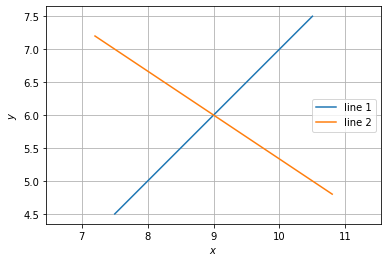
\includegraphics[width=\columnwidth]{solutions/quad/45/figure2.png}
\caption{Rhombus ABCD}
\label{quad/45/fig:Rhombus ABCD}
\end{figure}

    

\end{enumerate}
\item Show that points A=\myvec{a&b+c}, B=\myvec{b&c+a}, C=\myvec{c&a+b} are collinear.
\\
\solution 
%
\begin{align}
    E(X) &= \frac{1}{\sqrt{2\pi}} \int_{-\infty}^{\infty} x e^{-\frac{x^2}{2}}dx\\
    &=0 \quad \brak{ \text{ odd function}}
\end{align}
\begin{align}
    E\brak{X^2}&= \frac{1}{\sqrt{2\pi}}\int_{-\infty}^{\infty} x^2
e^ {-\frac{x^2}{2}} dx \quad \brak{even function}\\
    &= \frac{2}{\sqrt{2\pi}} \int_{0}^{\infty} x^2 e^{-\frac{x^2}{2}} dx\\
    &= \frac{2}{\sqrt{2\pi}}\int_{0}^{\infty}\sqrt{2u}e^{-u} du \quad\brak{Let \frac{x^2}{2}= u}\\
    &= \frac{2}{\sqrt{\pi}} \int_{0}^{\infty} e^{-u} u^{\frac{3}{2}-1} du\\
    &= \frac{2}{\sqrt{\pi}} \Gamma\brak{{\frac{3}{2}}}\\
    &= \frac{1}{\sqrt{\pi}}\Gamma\brak{\frac{1}{2}} \\
    &= 1
\end{align}
where we have used the fact that
\begin{align}
\quad\because \Gamma(n)= (n-1)\Gamma(n-1); \Gamma\brak{\frac{1}{2}}=\sqrt{\pi}
\end{align}
%
Thus, the  variance is
\begin{align}
    \sigma^2 =  E\brak X^2 - E^2\brak X = 1
\end{align}

\item Find values of k if area of triangle is 4sq.units and vertices are \\
(i) \myvec{k&0}, \myvec{4&0}, \myvec{0&2} \\ (ii) \myvec{-2&0}, \myvec{0&4}, \myvec{0&k}
\item (i) Find equation of line joining \myvec{1&2} and \myvec{3&6} using determinants.\\
(ii) Find equation of line joining \myvec{3&1} and \myvec{9&3} using determinants.
\item If the area of triangle is 35 sq.units with vertices \myvec{2&-6}, \myvec{5&4} and \myvec{k&4}.then k is 
\begin{enumerate}
\item 12
\item -2
\item -12,-2
\item 12,-2
\end{enumerate}

\textbf{Write Minors and Coafactors of the elements of following determinants:}
\item (i) $\begin{vmatrix}
2&-4 \\ 0 &3 \end{vmatrix}$ \\
(ii) $\begin{vmatrix}a&c \\ b &d\end{vmatrix}$
\item (i) $\begin{vmatrix}1&0&0 \\ 0&1&0 \\ 0&0&1\end{vmatrix}$\\
(ii) $\begin{vmatrix}1&0&4 \\ 3&5&-1 \\ 0&1&2\end{vmatrix}$
\item Using Cofactors of elements of second row,evaluate $\Delta$ =
$\begin{vmatrix} 5&3&8 \\ 2&0&1 \\ 1&2&3 \end{vmatrix}.$
\item Using Cofactors of elements of third column ,evaluate $\Delta$ = 
$\begin{vmatrix} 1&x&yz \\ 1&y&zx \\ 1&z&xy \end{vmatrix}.$
\item If $\Delta = \begin{vmatrix}
a_{11}&a_{12}&a_{13} \\ a_{21}&a_{22}&a_{23} \\ a_{31}&a_{32}&a_{33}
\end{vmatrix}$ and $A_{ij}$ is Cofactors of $a_{ij}$ then value of $\Delta$ is given by 
\begin{enumerate}
\item $a_{11}A_{31}+a_{12}A_{32}+a_{13}A_{33}$
\item $a_{11}A_{11}+a_{12}A_{21}+a_{13}A_{31}$
\item $a_{21}A_{11}+a_{22}A_{12}+a_{23}A_{13}$
\item $a_{11}A_{11}+a_{21}A_{21}+a_{31}A_{31}$
\end{enumerate} 
\textbf{Find adjoint of each of the matrices} 
\item $\begin{bmatrix}
1&2 \\ 3&4
\end{bmatrix}$
\item $\begin{bmatrix}
1&-1&2 \\ 2&3&5 \\ -2&0&1
\end{bmatrix}$
Verify A(adjA)=(adjA)A=$\abs{A}I$
\item $\begin{bmatrix}
2&3 \\ -4&-6
\end{bmatrix}$
\item $\begin{bmatrix}
1&-1&2 \\ 3&0&-2 \\ 1&0&3
\end{bmatrix}$
\item $\begin{bmatrix}
2&-2 \\ 4&3
\end{bmatrix}$
\item $\begin{bmatrix}
-1&5 \\ -3&2
\end{bmatrix}$
\item $\begin{bmatrix}
1&2&3 \\ 0&2&4 \\ 0&0&5
\end{bmatrix}$
\item $\begin{bmatrix}
1&0&0 \\ 3&3&0 \\ 5&2&-1
\end{bmatrix}$
\item $\begin{bmatrix}
2&1&3 \\ 4&-1&0 \\ -7&2&1
\end{bmatrix}$
\item $\begin{bmatrix}
1&-1&2 \\ 0&2&-3 \\ 3&-2&4
\end{bmatrix}$
\item $\begin{bmatrix}
1&0&0 \\ 0& \cos\alpha &\sin\alpha \\ 0&\sin\alpha&-\cos\alpha
\end{bmatrix}$
\item Let A=
$\begin{bmatrix}
3&7 \\ 2&5
\end{bmatrix}$ and B=
$\begin{bmatrix}
6&8 \\ 7&9
\end{bmatrix}.$ Verify that $(AB)^{-1}=B^{-1} A^{-1}$
\item Let A =$\begin{bmatrix}
3&1 \\ -1&2
\end{bmatrix},$ show that $A^2-5A+7I=O.$ Hence find $A^{-1}$
\solution 
%
\begin{align}
    E(X) &= \frac{1}{\sqrt{2\pi}} \int_{-\infty}^{\infty} x e^{-\frac{x^2}{2}}dx\\
    &=0 \quad \brak{ \text{ odd function}}
\end{align}
\begin{align}
    E\brak{X^2}&= \frac{1}{\sqrt{2\pi}}\int_{-\infty}^{\infty} x^2
e^ {-\frac{x^2}{2}} dx \quad \brak{even function}\\
    &= \frac{2}{\sqrt{2\pi}} \int_{0}^{\infty} x^2 e^{-\frac{x^2}{2}} dx\\
    &= \frac{2}{\sqrt{2\pi}}\int_{0}^{\infty}\sqrt{2u}e^{-u} du \quad\brak{Let \frac{x^2}{2}= u}\\
    &= \frac{2}{\sqrt{\pi}} \int_{0}^{\infty} e^{-u} u^{\frac{3}{2}-1} du\\
    &= \frac{2}{\sqrt{\pi}} \Gamma\brak{{\frac{3}{2}}}\\
    &= \frac{1}{\sqrt{\pi}}\Gamma\brak{\frac{1}{2}} \\
    &= 1
\end{align}
where we have used the fact that
\begin{align}
\quad\because \Gamma(n)= (n-1)\Gamma(n-1); \Gamma\brak{\frac{1}{2}}=\sqrt{\pi}
\end{align}
%
Thus, the  variance is
\begin{align}
    \sigma^2 =  E\brak X^2 - E^2\brak X = 1
\end{align}

\item For the matrix A= $\begin{bmatrix}
3&2 \\ 1&1
\end{bmatrix},$ find the numbers a and b such that $A^2+aA+bI=O.$
\\
\solution 
%
\begin{align}
    E(X) &= \frac{1}{\sqrt{2\pi}} \int_{-\infty}^{\infty} x e^{-\frac{x^2}{2}}dx\\
    &=0 \quad \brak{ \text{ odd function}}
\end{align}
\begin{align}
    E\brak{X^2}&= \frac{1}{\sqrt{2\pi}}\int_{-\infty}^{\infty} x^2
e^ {-\frac{x^2}{2}} dx \quad \brak{even function}\\
    &= \frac{2}{\sqrt{2\pi}} \int_{0}^{\infty} x^2 e^{-\frac{x^2}{2}} dx\\
    &= \frac{2}{\sqrt{2\pi}}\int_{0}^{\infty}\sqrt{2u}e^{-u} du \quad\brak{Let \frac{x^2}{2}= u}\\
    &= \frac{2}{\sqrt{\pi}} \int_{0}^{\infty} e^{-u} u^{\frac{3}{2}-1} du\\
    &= \frac{2}{\sqrt{\pi}} \Gamma\brak{{\frac{3}{2}}}\\
    &= \frac{1}{\sqrt{\pi}}\Gamma\brak{\frac{1}{2}} \\
    &= 1
\end{align}
where we have used the fact that
\begin{align}
\quad\because \Gamma(n)= (n-1)\Gamma(n-1); \Gamma\brak{\frac{1}{2}}=\sqrt{\pi}
\end{align}
%
Thus, the  variance is
\begin{align}
    \sigma^2 =  E\brak X^2 - E^2\brak X = 1
\end{align}


\item For the matrix A=$\myvec{1&1&1 \\ 1&2&-3 \\ 2&-1&3}$.Show that \begin{align}
    A^3-6A^2+5A+11I=0\label{eq:det/49/1}
\end{align} and hence find $A^{-1}$.
%\item For the matrix A=$\begin{bmatrix}
%1&1&1 \\ 1&2&-3 \\ 2&-1&3
%\end{bmatrix}$ Show that $A^3-6A^2+9A-4I=O$ and hence find $A^{-1}$
\solution 
%
\begin{align}
    E(X) &= \frac{1}{\sqrt{2\pi}} \int_{-\infty}^{\infty} x e^{-\frac{x^2}{2}}dx\\
    &=0 \quad \brak{ \text{ odd function}}
\end{align}
\begin{align}
    E\brak{X^2}&= \frac{1}{\sqrt{2\pi}}\int_{-\infty}^{\infty} x^2
e^ {-\frac{x^2}{2}} dx \quad \brak{even function}\\
    &= \frac{2}{\sqrt{2\pi}} \int_{0}^{\infty} x^2 e^{-\frac{x^2}{2}} dx\\
    &= \frac{2}{\sqrt{2\pi}}\int_{0}^{\infty}\sqrt{2u}e^{-u} du \quad\brak{Let \frac{x^2}{2}= u}\\
    &= \frac{2}{\sqrt{\pi}} \int_{0}^{\infty} e^{-u} u^{\frac{3}{2}-1} du\\
    &= \frac{2}{\sqrt{\pi}} \Gamma\brak{{\frac{3}{2}}}\\
    &= \frac{1}{\sqrt{\pi}}\Gamma\brak{\frac{1}{2}} \\
    &= 1
\end{align}
where we have used the fact that
\begin{align}
\quad\because \Gamma(n)= (n-1)\Gamma(n-1); \Gamma\brak{\frac{1}{2}}=\sqrt{\pi}
\end{align}
%
Thus, the  variance is
\begin{align}
    \sigma^2 =  E\brak X^2 - E^2\brak X = 1
\end{align}

\item Let A be a nonsingular square matrix of order 3X3 .Then $\abs{adjA}$ is equal to 
\begin{enumerate}
\item $\abs{A}$
\item $\abs{A}^2$
\item $\abs{A}^3$
\item $3\abs{A}$
\end{enumerate}
\item If A is an invertible matrix of order 2, then det($A^{-1}$) is equal to 
\begin{enumerate}
\item det(A)
\item $\frac{1}{det(A)}$
\item 1
\item 0
\end{enumerate}
\textbf{Examine the consistency of the system of given Equations.}
\item $\begin{alignedat}[t]{2}
x+3y&=5 
\\
2x+6y&=8 
\end{alignedat}$\\
\\
\solution 
%
\begin{align}
    E(X) &= \frac{1}{\sqrt{2\pi}} \int_{-\infty}^{\infty} x e^{-\frac{x^2}{2}}dx\\
    &=0 \quad \brak{ \text{ odd function}}
\end{align}
\begin{align}
    E\brak{X^2}&= \frac{1}{\sqrt{2\pi}}\int_{-\infty}^{\infty} x^2
e^ {-\frac{x^2}{2}} dx \quad \brak{even function}\\
    &= \frac{2}{\sqrt{2\pi}} \int_{0}^{\infty} x^2 e^{-\frac{x^2}{2}} dx\\
    &= \frac{2}{\sqrt{2\pi}}\int_{0}^{\infty}\sqrt{2u}e^{-u} du \quad\brak{Let \frac{x^2}{2}= u}\\
    &= \frac{2}{\sqrt{\pi}} \int_{0}^{\infty} e^{-u} u^{\frac{3}{2}-1} du\\
    &= \frac{2}{\sqrt{\pi}} \Gamma\brak{{\frac{3}{2}}}\\
    &= \frac{1}{\sqrt{\pi}}\Gamma\brak{\frac{1}{2}} \\
    &= 1
\end{align}
where we have used the fact that
\begin{align}
\quad\because \Gamma(n)= (n-1)\Gamma(n-1); \Gamma\brak{\frac{1}{2}}=\sqrt{\pi}
\end{align}
%
Thus, the  variance is
\begin{align}
    \sigma^2 =  E\brak X^2 - E^2\brak X = 1
\end{align}

\item x+y+z=1\\ 2x+3y+2z=2\\ax+ay+2az=4\\
\\
\solution 
%
\begin{align}
    E(X) &= \frac{1}{\sqrt{2\pi}} \int_{-\infty}^{\infty} x e^{-\frac{x^2}{2}}dx\\
    &=0 \quad \brak{ \text{ odd function}}
\end{align}
\begin{align}
    E\brak{X^2}&= \frac{1}{\sqrt{2\pi}}\int_{-\infty}^{\infty} x^2
e^ {-\frac{x^2}{2}} dx \quad \brak{even function}\\
    &= \frac{2}{\sqrt{2\pi}} \int_{0}^{\infty} x^2 e^{-\frac{x^2}{2}} dx\\
    &= \frac{2}{\sqrt{2\pi}}\int_{0}^{\infty}\sqrt{2u}e^{-u} du \quad\brak{Let \frac{x^2}{2}= u}\\
    &= \frac{2}{\sqrt{\pi}} \int_{0}^{\infty} e^{-u} u^{\frac{3}{2}-1} du\\
    &= \frac{2}{\sqrt{\pi}} \Gamma\brak{{\frac{3}{2}}}\\
    &= \frac{1}{\sqrt{\pi}}\Gamma\brak{\frac{1}{2}} \\
    &= 1
\end{align}
where we have used the fact that
\begin{align}
\quad\because \Gamma(n)= (n-1)\Gamma(n-1); \Gamma\brak{\frac{1}{2}}=\sqrt{\pi}
\end{align}
%
Thus, the  variance is
\begin{align}
    \sigma^2 =  E\brak X^2 - E^2\brak X = 1
\end{align}

\item 3x-y-2z=2 \\ 2y-z=-1 \\ 3x-5y=3\\
\\
\solution 
%
\begin{align}
    E(X) &= \frac{1}{\sqrt{2\pi}} \int_{-\infty}^{\infty} x e^{-\frac{x^2}{2}}dx\\
    &=0 \quad \brak{ \text{ odd function}}
\end{align}
\begin{align}
    E\brak{X^2}&= \frac{1}{\sqrt{2\pi}}\int_{-\infty}^{\infty} x^2
e^ {-\frac{x^2}{2}} dx \quad \brak{even function}\\
    &= \frac{2}{\sqrt{2\pi}} \int_{0}^{\infty} x^2 e^{-\frac{x^2}{2}} dx\\
    &= \frac{2}{\sqrt{2\pi}}\int_{0}^{\infty}\sqrt{2u}e^{-u} du \quad\brak{Let \frac{x^2}{2}= u}\\
    &= \frac{2}{\sqrt{\pi}} \int_{0}^{\infty} e^{-u} u^{\frac{3}{2}-1} du\\
    &= \frac{2}{\sqrt{\pi}} \Gamma\brak{{\frac{3}{2}}}\\
    &= \frac{1}{\sqrt{\pi}}\Gamma\brak{\frac{1}{2}} \\
    &= 1
\end{align}
where we have used the fact that
\begin{align}
\quad\because \Gamma(n)= (n-1)\Gamma(n-1); \Gamma\brak{\frac{1}{2}}=\sqrt{\pi}
\end{align}
%
Thus, the  variance is
\begin{align}
    \sigma^2 =  E\brak X^2 - E^2\brak X = 1
\end{align}

\item 5x-y+4z=5 \\ 2x+3y+5z=2 \\ 5x-2y+6z=-1\\
\\
\solution
%
\begin{align}
    E(X) &= \frac{1}{\sqrt{2\pi}} \int_{-\infty}^{\infty} x e^{-\frac{x^2}{2}}dx\\
    &=0 \quad \brak{ \text{ odd function}}
\end{align}
\begin{align}
    E\brak{X^2}&= \frac{1}{\sqrt{2\pi}}\int_{-\infty}^{\infty} x^2
e^ {-\frac{x^2}{2}} dx \quad \brak{even function}\\
    &= \frac{2}{\sqrt{2\pi}} \int_{0}^{\infty} x^2 e^{-\frac{x^2}{2}} dx\\
    &= \frac{2}{\sqrt{2\pi}}\int_{0}^{\infty}\sqrt{2u}e^{-u} du \quad\brak{Let \frac{x^2}{2}= u}\\
    &= \frac{2}{\sqrt{\pi}} \int_{0}^{\infty} e^{-u} u^{\frac{3}{2}-1} du\\
    &= \frac{2}{\sqrt{\pi}} \Gamma\brak{{\frac{3}{2}}}\\
    &= \frac{1}{\sqrt{\pi}}\Gamma\brak{\frac{1}{2}} \\
    &= 1
\end{align}
where we have used the fact that
\begin{align}
\quad\because \Gamma(n)= (n-1)\Gamma(n-1); \Gamma\brak{\frac{1}{2}}=\sqrt{\pi}
\end{align}
%
Thus, the  variance is
\begin{align}
    \sigma^2 =  E\brak X^2 - E^2\brak X = 1
\end{align}

Solve the system linear equations,using matrix method.
\item 
$\begin{alignedat}[t]{2}
%\myvec{5 & 2}\vec{x} &= 4
%\\ 
%\myvec{7 & 3}\vec{x} &= 5
5x+2y&=4 \\ 7x+3y&=5
\end{alignedat}$
\\
\solution
%
\begin{align}
    E(X) &= \frac{1}{\sqrt{2\pi}} \int_{-\infty}^{\infty} x e^{-\frac{x^2}{2}}dx\\
    &=0 \quad \brak{ \text{ odd function}}
\end{align}
\begin{align}
    E\brak{X^2}&= \frac{1}{\sqrt{2\pi}}\int_{-\infty}^{\infty} x^2
e^ {-\frac{x^2}{2}} dx \quad \brak{even function}\\
    &= \frac{2}{\sqrt{2\pi}} \int_{0}^{\infty} x^2 e^{-\frac{x^2}{2}} dx\\
    &= \frac{2}{\sqrt{2\pi}}\int_{0}^{\infty}\sqrt{2u}e^{-u} du \quad\brak{Let \frac{x^2}{2}= u}\\
    &= \frac{2}{\sqrt{\pi}} \int_{0}^{\infty} e^{-u} u^{\frac{3}{2}-1} du\\
    &= \frac{2}{\sqrt{\pi}} \Gamma\brak{{\frac{3}{2}}}\\
    &= \frac{1}{\sqrt{\pi}}\Gamma\brak{\frac{1}{2}} \\
    &= 1
\end{align}
where we have used the fact that
\begin{align}
\quad\because \Gamma(n)= (n-1)\Gamma(n-1); \Gamma\brak{\frac{1}{2}}=\sqrt{\pi}
\end{align}
%
Thus, the  variance is
\begin{align}
    \sigma^2 =  E\brak X^2 - E^2\brak X = 1
\end{align}

\item 
$\begin{alignedat}[t]{2}
%\myvec{2 & -1}\vec{x} &= -2
%\\ 
%\myvec{3 & 4}\vec{x} &= 3
2x-y&=-2 \\ 3x+4y&=3
\end{alignedat}$
\\
\solution
%
\begin{align}
    E(X) &= \frac{1}{\sqrt{2\pi}} \int_{-\infty}^{\infty} x e^{-\frac{x^2}{2}}dx\\
    &=0 \quad \brak{ \text{ odd function}}
\end{align}
\begin{align}
    E\brak{X^2}&= \frac{1}{\sqrt{2\pi}}\int_{-\infty}^{\infty} x^2
e^ {-\frac{x^2}{2}} dx \quad \brak{even function}\\
    &= \frac{2}{\sqrt{2\pi}} \int_{0}^{\infty} x^2 e^{-\frac{x^2}{2}} dx\\
    &= \frac{2}{\sqrt{2\pi}}\int_{0}^{\infty}\sqrt{2u}e^{-u} du \quad\brak{Let \frac{x^2}{2}= u}\\
    &= \frac{2}{\sqrt{\pi}} \int_{0}^{\infty} e^{-u} u^{\frac{3}{2}-1} du\\
    &= \frac{2}{\sqrt{\pi}} \Gamma\brak{{\frac{3}{2}}}\\
    &= \frac{1}{\sqrt{\pi}}\Gamma\brak{\frac{1}{2}} \\
    &= 1
\end{align}
where we have used the fact that
\begin{align}
\quad\because \Gamma(n)= (n-1)\Gamma(n-1); \Gamma\brak{\frac{1}{2}}=\sqrt{\pi}
\end{align}
%
Thus, the  variance is
\begin{align}
    \sigma^2 =  E\brak X^2 - E^2\brak X = 1
\end{align}

\item $\begin{alignedat}[t]{2}
%\myvec{4 & -3}\vec{x} &= 3
%\\ 
%\myvec{3 & -5}\vec{x} &= 7
4x-3y&=3 \\ 3x-5y&=7
\end{alignedat}$
\\
\solution
%
\begin{align}
    E(X) &= \frac{1}{\sqrt{2\pi}} \int_{-\infty}^{\infty} x e^{-\frac{x^2}{2}}dx\\
    &=0 \quad \brak{ \text{ odd function}}
\end{align}
\begin{align}
    E\brak{X^2}&= \frac{1}{\sqrt{2\pi}}\int_{-\infty}^{\infty} x^2
e^ {-\frac{x^2}{2}} dx \quad \brak{even function}\\
    &= \frac{2}{\sqrt{2\pi}} \int_{0}^{\infty} x^2 e^{-\frac{x^2}{2}} dx\\
    &= \frac{2}{\sqrt{2\pi}}\int_{0}^{\infty}\sqrt{2u}e^{-u} du \quad\brak{Let \frac{x^2}{2}= u}\\
    &= \frac{2}{\sqrt{\pi}} \int_{0}^{\infty} e^{-u} u^{\frac{3}{2}-1} du\\
    &= \frac{2}{\sqrt{\pi}} \Gamma\brak{{\frac{3}{2}}}\\
    &= \frac{1}{\sqrt{\pi}}\Gamma\brak{\frac{1}{2}} \\
    &= 1
\end{align}
where we have used the fact that
\begin{align}
\quad\because \Gamma(n)= (n-1)\Gamma(n-1); \Gamma\brak{\frac{1}{2}}=\sqrt{\pi}
\end{align}
%
Thus, the  variance is
\begin{align}
    \sigma^2 =  E\brak X^2 - E^2\brak X = 1
\end{align}

\item $\begin{alignedat}[t]{2}
%\myvec{5 & 2}\vec{x} &= 3
%\\ 
%\myvec{3 & 2}\vec{x} &= 5
5x+2y&=3 \\ 3x+2y&=5
\end{alignedat}$\\
\\
\solution
%
\begin{align}
    E(X) &= \frac{1}{\sqrt{2\pi}} \int_{-\infty}^{\infty} x e^{-\frac{x^2}{2}}dx\\
    &=0 \quad \brak{ \text{ odd function}}
\end{align}
\begin{align}
    E\brak{X^2}&= \frac{1}{\sqrt{2\pi}}\int_{-\infty}^{\infty} x^2
e^ {-\frac{x^2}{2}} dx \quad \brak{even function}\\
    &= \frac{2}{\sqrt{2\pi}} \int_{0}^{\infty} x^2 e^{-\frac{x^2}{2}} dx\\
    &= \frac{2}{\sqrt{2\pi}}\int_{0}^{\infty}\sqrt{2u}e^{-u} du \quad\brak{Let \frac{x^2}{2}= u}\\
    &= \frac{2}{\sqrt{\pi}} \int_{0}^{\infty} e^{-u} u^{\frac{3}{2}-1} du\\
    &= \frac{2}{\sqrt{\pi}} \Gamma\brak{{\frac{3}{2}}}\\
    &= \frac{1}{\sqrt{\pi}}\Gamma\brak{\frac{1}{2}} \\
    &= 1
\end{align}
where we have used the fact that
\begin{align}
\quad\because \Gamma(n)= (n-1)\Gamma(n-1); \Gamma\brak{\frac{1}{2}}=\sqrt{\pi}
\end{align}
%
Thus, the  variance is
\begin{align}
    \sigma^2 =  E\brak X^2 - E^2\brak X = 1
\end{align}

\item 2x+y+z = 1 \\ x-2y-z = $\frac{3}{2}$ \\ 3y- 5z = 9\\
\item x-y+z = 4 \\ 2x+y-3z = 0 \\ x+y+z = 2\\
\item 2x+3y+3z = 5 \\ x-2y+z = -4 \\ 3x-y-2z = 3\\
\item x-y+2z = 7 \\ 3x+4y-5z = -5 \\ 2x-y+3z = 12\\ 
\item If A=$\begin{bmatrix}
2&-3&5 \\ 3&2&-4 \\ 1&1&-2
\end{bmatrix},$ find $A^{-1}.$ Using $A^{-1}$ solve the system of equations \\
2x-3y+5z = 11, \\ 3x+2y-4z = -5, \\ x+y-2z =-3.\\
\item The cost of 4 kg onion, 3 kg wheat and 2 kg rice is \rupee 60. The cost of 2 kg onion,4 kg wheat and 6 kg rice is \rupee 90.The cost of 6kg onion 2kg wheat and 3kg rice is \rupee 70.Find the cost of each item per kg by matrix mathod. 
\item Prove that the determinant \\
$\begin{vmatrix}
x &\sin\theta&\cos\theta \\ -\sin\theta&-x&1 \\ \cos\theta&1&x
\end{vmatrix}$ 
is independent of $\theta$
\\
\solution 
%
\begin{align}
    E(X) &= \frac{1}{\sqrt{2\pi}} \int_{-\infty}^{\infty} x e^{-\frac{x^2}{2}}dx\\
    &=0 \quad \brak{ \text{ odd function}}
\end{align}
\begin{align}
    E\brak{X^2}&= \frac{1}{\sqrt{2\pi}}\int_{-\infty}^{\infty} x^2
e^ {-\frac{x^2}{2}} dx \quad \brak{even function}\\
    &= \frac{2}{\sqrt{2\pi}} \int_{0}^{\infty} x^2 e^{-\frac{x^2}{2}} dx\\
    &= \frac{2}{\sqrt{2\pi}}\int_{0}^{\infty}\sqrt{2u}e^{-u} du \quad\brak{Let \frac{x^2}{2}= u}\\
    &= \frac{2}{\sqrt{\pi}} \int_{0}^{\infty} e^{-u} u^{\frac{3}{2}-1} du\\
    &= \frac{2}{\sqrt{\pi}} \Gamma\brak{{\frac{3}{2}}}\\
    &= \frac{1}{\sqrt{\pi}}\Gamma\brak{\frac{1}{2}} \\
    &= 1
\end{align}
where we have used the fact that
\begin{align}
\quad\because \Gamma(n)= (n-1)\Gamma(n-1); \Gamma\brak{\frac{1}{2}}=\sqrt{\pi}
\end{align}
%
Thus, the  variance is
\begin{align}
    \sigma^2 =  E\brak X^2 - E^2\brak X = 1
\end{align}


\item Without expanding the determinant, prove that\\ $\begin{vmatrix}
a&a^2&bc \\ b&b^2&ca \\c&c^2&ab
\end{vmatrix}=\begin{vmatrix}
1&a^2&a^3 \\ 1&b^2&b^3 \\ 1&c^2&c^3
\end{vmatrix}$.
\\
\solution
%%
\begin{align}
    E(X) &= \frac{1}{\sqrt{2\pi}} \int_{-\infty}^{\infty} x e^{-\frac{x^2}{2}}dx\\
    &=0 \quad \brak{ \text{ odd function}}
\end{align}
\begin{align}
    E\brak{X^2}&= \frac{1}{\sqrt{2\pi}}\int_{-\infty}^{\infty} x^2
e^ {-\frac{x^2}{2}} dx \quad \brak{even function}\\
    &= \frac{2}{\sqrt{2\pi}} \int_{0}^{\infty} x^2 e^{-\frac{x^2}{2}} dx\\
    &= \frac{2}{\sqrt{2\pi}}\int_{0}^{\infty}\sqrt{2u}e^{-u} du \quad\brak{Let \frac{x^2}{2}= u}\\
    &= \frac{2}{\sqrt{\pi}} \int_{0}^{\infty} e^{-u} u^{\frac{3}{2}-1} du\\
    &= \frac{2}{\sqrt{\pi}} \Gamma\brak{{\frac{3}{2}}}\\
    &= \frac{1}{\sqrt{\pi}}\Gamma\brak{\frac{1}{2}} \\
    &= 1
\end{align}
where we have used the fact that
\begin{align}
\quad\because \Gamma(n)= (n-1)\Gamma(n-1); \Gamma\brak{\frac{1}{2}}=\sqrt{\pi}
\end{align}
%
Thus, the  variance is
\begin{align}
    \sigma^2 =  E\brak X^2 - E^2\brak X = 1
\end{align}

\item Evaluate 
$\begin{vmatrix}
\cos\alpha \cos\beta &\cos\alpha \sin\beta &-\sin\alpha \\ -\sin\beta & \cos\beta &0 \\ \sin\alpha\cos\beta&\sin\alpha\sin\beta&\cos\alpha
\end{vmatrix}.$\\
\solution 
%
\begin{align}
    E(X) &= \frac{1}{\sqrt{2\pi}} \int_{-\infty}^{\infty} x e^{-\frac{x^2}{2}}dx\\
    &=0 \quad \brak{ \text{ odd function}}
\end{align}
\begin{align}
    E\brak{X^2}&= \frac{1}{\sqrt{2\pi}}\int_{-\infty}^{\infty} x^2
e^ {-\frac{x^2}{2}} dx \quad \brak{even function}\\
    &= \frac{2}{\sqrt{2\pi}} \int_{0}^{\infty} x^2 e^{-\frac{x^2}{2}} dx\\
    &= \frac{2}{\sqrt{2\pi}}\int_{0}^{\infty}\sqrt{2u}e^{-u} du \quad\brak{Let \frac{x^2}{2}= u}\\
    &= \frac{2}{\sqrt{\pi}} \int_{0}^{\infty} e^{-u} u^{\frac{3}{2}-1} du\\
    &= \frac{2}{\sqrt{\pi}} \Gamma\brak{{\frac{3}{2}}}\\
    &= \frac{1}{\sqrt{\pi}}\Gamma\brak{\frac{1}{2}} \\
    &= 1
\end{align}
where we have used the fact that
\begin{align}
\quad\because \Gamma(n)= (n-1)\Gamma(n-1); \Gamma\brak{\frac{1}{2}}=\sqrt{\pi}
\end{align}
%
Thus, the  variance is
\begin{align}
    \sigma^2 =  E\brak X^2 - E^2\brak X = 1
\end{align}

\item If a,b and c are real numbers, and \\$\Delta=\begin{vmatrix}
b+c&c=a&a=b \\ c+a&a+b&b+c \\ a+b&b+c&c+a
\end{vmatrix}=0,$ Show that either a+b+c=0 or a=b=c.\\
\solution 
%
\begin{align}
    E(X) &= \frac{1}{\sqrt{2\pi}} \int_{-\infty}^{\infty} x e^{-\frac{x^2}{2}}dx\\
    &=0 \quad \brak{ \text{ odd function}}
\end{align}
\begin{align}
    E\brak{X^2}&= \frac{1}{\sqrt{2\pi}}\int_{-\infty}^{\infty} x^2
e^ {-\frac{x^2}{2}} dx \quad \brak{even function}\\
    &= \frac{2}{\sqrt{2\pi}} \int_{0}^{\infty} x^2 e^{-\frac{x^2}{2}} dx\\
    &= \frac{2}{\sqrt{2\pi}}\int_{0}^{\infty}\sqrt{2u}e^{-u} du \quad\brak{Let \frac{x^2}{2}= u}\\
    &= \frac{2}{\sqrt{\pi}} \int_{0}^{\infty} e^{-u} u^{\frac{3}{2}-1} du\\
    &= \frac{2}{\sqrt{\pi}} \Gamma\brak{{\frac{3}{2}}}\\
    &= \frac{1}{\sqrt{\pi}}\Gamma\brak{\frac{1}{2}} \\
    &= 1
\end{align}
where we have used the fact that
\begin{align}
\quad\because \Gamma(n)= (n-1)\Gamma(n-1); \Gamma\brak{\frac{1}{2}}=\sqrt{\pi}
\end{align}
%
Thus, the  variance is
\begin{align}
    \sigma^2 =  E\brak X^2 - E^2\brak X = 1
\end{align}

\item Solve the equation\\ $\begin{vmatrix}
x+a&x&x \\ x&x+a&x \\ x&x&x+a
\end{vmatrix}=0, a\neq0$\\
\solution 
%
\begin{align}
    E(X) &= \frac{1}{\sqrt{2\pi}} \int_{-\infty}^{\infty} x e^{-\frac{x^2}{2}}dx\\
    &=0 \quad \brak{ \text{ odd function}}
\end{align}
\begin{align}
    E\brak{X^2}&= \frac{1}{\sqrt{2\pi}}\int_{-\infty}^{\infty} x^2
e^ {-\frac{x^2}{2}} dx \quad \brak{even function}\\
    &= \frac{2}{\sqrt{2\pi}} \int_{0}^{\infty} x^2 e^{-\frac{x^2}{2}} dx\\
    &= \frac{2}{\sqrt{2\pi}}\int_{0}^{\infty}\sqrt{2u}e^{-u} du \quad\brak{Let \frac{x^2}{2}= u}\\
    &= \frac{2}{\sqrt{\pi}} \int_{0}^{\infty} e^{-u} u^{\frac{3}{2}-1} du\\
    &= \frac{2}{\sqrt{\pi}} \Gamma\brak{{\frac{3}{2}}}\\
    &= \frac{1}{\sqrt{\pi}}\Gamma\brak{\frac{1}{2}} \\
    &= 1
\end{align}
where we have used the fact that
\begin{align}
\quad\because \Gamma(n)= (n-1)\Gamma(n-1); \Gamma\brak{\frac{1}{2}}=\sqrt{\pi}
\end{align}
%
Thus, the  variance is
\begin{align}
    \sigma^2 =  E\brak X^2 - E^2\brak X = 1
\end{align}

\item Prove that \\
$\begin{vmatrix}
a^2&bc&ac+c^2 \\ a^2+ab&b^2&ac \\ab&b^2+bc&c^2
\end{vmatrix}= 4a^2b^2c^2$\\
\solution 
%
\begin{align}
    E(X) &= \frac{1}{\sqrt{2\pi}} \int_{-\infty}^{\infty} x e^{-\frac{x^2}{2}}dx\\
    &=0 \quad \brak{ \text{ odd function}}
\end{align}
\begin{align}
    E\brak{X^2}&= \frac{1}{\sqrt{2\pi}}\int_{-\infty}^{\infty} x^2
e^ {-\frac{x^2}{2}} dx \quad \brak{even function}\\
    &= \frac{2}{\sqrt{2\pi}} \int_{0}^{\infty} x^2 e^{-\frac{x^2}{2}} dx\\
    &= \frac{2}{\sqrt{2\pi}}\int_{0}^{\infty}\sqrt{2u}e^{-u} du \quad\brak{Let \frac{x^2}{2}= u}\\
    &= \frac{2}{\sqrt{\pi}} \int_{0}^{\infty} e^{-u} u^{\frac{3}{2}-1} du\\
    &= \frac{2}{\sqrt{\pi}} \Gamma\brak{{\frac{3}{2}}}\\
    &= \frac{1}{\sqrt{\pi}}\Gamma\brak{\frac{1}{2}} \\
    &= 1
\end{align}
where we have used the fact that
\begin{align}
\quad\because \Gamma(n)= (n-1)\Gamma(n-1); \Gamma\brak{\frac{1}{2}}=\sqrt{\pi}
\end{align}
%
Thus, the  variance is
\begin{align}
    \sigma^2 =  E\brak X^2 - E^2\brak X = 1
\end{align}

\item If \\
$A^{-1}=\begin{bmatrix}
3&-1&1 \\ -15&6&-5 \\5&-2&2
\end{bmatrix}$ and B=$\begin{bmatrix}
1&2&-2 \\ -1&3&0 \\0&-2&1
\end{bmatrix},$ find $(AB)^{-1}$\\
\item Let A=
$\begin{bmatrix}
1&2&1 \\ 2&3&1 \\1&1&5
\end{bmatrix}.$ Verify that \\
(i) $[adj A]^{-1}=adj(A)^{-1}$\\
(ii) $(A^{-1})^{-1}=A$\\
\item Evaluate 
$\begin{vmatrix}
x&y&x+y \\ y&x+y&x \\ x+y&x&y
\end{vmatrix}$\\
\solution 
%
\begin{align}
    E(X) &= \frac{1}{\sqrt{2\pi}} \int_{-\infty}^{\infty} x e^{-\frac{x^2}{2}}dx\\
    &=0 \quad \brak{ \text{ odd function}}
\end{align}
\begin{align}
    E\brak{X^2}&= \frac{1}{\sqrt{2\pi}}\int_{-\infty}^{\infty} x^2
e^ {-\frac{x^2}{2}} dx \quad \brak{even function}\\
    &= \frac{2}{\sqrt{2\pi}} \int_{0}^{\infty} x^2 e^{-\frac{x^2}{2}} dx\\
    &= \frac{2}{\sqrt{2\pi}}\int_{0}^{\infty}\sqrt{2u}e^{-u} du \quad\brak{Let \frac{x^2}{2}= u}\\
    &= \frac{2}{\sqrt{\pi}} \int_{0}^{\infty} e^{-u} u^{\frac{3}{2}-1} du\\
    &= \frac{2}{\sqrt{\pi}} \Gamma\brak{{\frac{3}{2}}}\\
    &= \frac{1}{\sqrt{\pi}}\Gamma\brak{\frac{1}{2}} \\
    &= 1
\end{align}
where we have used the fact that
\begin{align}
\quad\because \Gamma(n)= (n-1)\Gamma(n-1); \Gamma\brak{\frac{1}{2}}=\sqrt{\pi}
\end{align}
%
Thus, the  variance is
\begin{align}
    \sigma^2 =  E\brak X^2 - E^2\brak X = 1
\end{align}

\item Evaluate 
$\begin{vmatrix}
1&x&y \\ 1&x+y&y \\ 1&x&x+y
\end{vmatrix}$
\solution 
%
\begin{align}
    E(X) &= \frac{1}{\sqrt{2\pi}} \int_{-\infty}^{\infty} x e^{-\frac{x^2}{2}}dx\\
    &=0 \quad \brak{ \text{ odd function}}
\end{align}
\begin{align}
    E\brak{X^2}&= \frac{1}{\sqrt{2\pi}}\int_{-\infty}^{\infty} x^2
e^ {-\frac{x^2}{2}} dx \quad \brak{even function}\\
    &= \frac{2}{\sqrt{2\pi}} \int_{0}^{\infty} x^2 e^{-\frac{x^2}{2}} dx\\
    &= \frac{2}{\sqrt{2\pi}}\int_{0}^{\infty}\sqrt{2u}e^{-u} du \quad\brak{Let \frac{x^2}{2}= u}\\
    &= \frac{2}{\sqrt{\pi}} \int_{0}^{\infty} e^{-u} u^{\frac{3}{2}-1} du\\
    &= \frac{2}{\sqrt{\pi}} \Gamma\brak{{\frac{3}{2}}}\\
    &= \frac{1}{\sqrt{\pi}}\Gamma\brak{\frac{1}{2}} \\
    &= 1
\end{align}
where we have used the fact that
\begin{align}
\quad\because \Gamma(n)= (n-1)\Gamma(n-1); \Gamma\brak{\frac{1}{2}}=\sqrt{\pi}
\end{align}
%
Thus, the  variance is
\begin{align}
    \sigma^2 =  E\brak X^2 - E^2\brak X = 1
\end{align}

Using properties of determinants ,prove that:\\
\item $\begin{vmatrix}
\alpha&\alpha^2&\beta+\gamma \\ \beta&\beta^2&\gamma+\alpha \\ \gamma&\gamma^2&\alpha+\beta
\end{vmatrix}=(\beta-\gamma)(\gamma-\alpha)(\alpha-\beta)(\alpha+\beta+\gamma)$\\
\solution 
%
\begin{align}
    E(X) &= \frac{1}{\sqrt{2\pi}} \int_{-\infty}^{\infty} x e^{-\frac{x^2}{2}}dx\\
    &=0 \quad \brak{ \text{ odd function}}
\end{align}
\begin{align}
    E\brak{X^2}&= \frac{1}{\sqrt{2\pi}}\int_{-\infty}^{\infty} x^2
e^ {-\frac{x^2}{2}} dx \quad \brak{even function}\\
    &= \frac{2}{\sqrt{2\pi}} \int_{0}^{\infty} x^2 e^{-\frac{x^2}{2}} dx\\
    &= \frac{2}{\sqrt{2\pi}}\int_{0}^{\infty}\sqrt{2u}e^{-u} du \quad\brak{Let \frac{x^2}{2}= u}\\
    &= \frac{2}{\sqrt{\pi}} \int_{0}^{\infty} e^{-u} u^{\frac{3}{2}-1} du\\
    &= \frac{2}{\sqrt{\pi}} \Gamma\brak{{\frac{3}{2}}}\\
    &= \frac{1}{\sqrt{\pi}}\Gamma\brak{\frac{1}{2}} \\
    &= 1
\end{align}
where we have used the fact that
\begin{align}
\quad\because \Gamma(n)= (n-1)\Gamma(n-1); \Gamma\brak{\frac{1}{2}}=\sqrt{\pi}
\end{align}
%
Thus, the  variance is
\begin{align}
    \sigma^2 =  E\brak X^2 - E^2\brak X = 1
\end{align}

\item $\begin{vmatrix}
x&x^2&1+px^3 \\ y&y^2&1+py^3 \\z&z^2&1+pz^3
\end{vmatrix}=(1+pxyz)(x-y)(y-z)(z-x),$ where p is any scalar.\\
\solution 
%
\begin{align}
    E(X) &= \frac{1}{\sqrt{2\pi}} \int_{-\infty}^{\infty} x e^{-\frac{x^2}{2}}dx\\
    &=0 \quad \brak{ \text{ odd function}}
\end{align}
\begin{align}
    E\brak{X^2}&= \frac{1}{\sqrt{2\pi}}\int_{-\infty}^{\infty} x^2
e^ {-\frac{x^2}{2}} dx \quad \brak{even function}\\
    &= \frac{2}{\sqrt{2\pi}} \int_{0}^{\infty} x^2 e^{-\frac{x^2}{2}} dx\\
    &= \frac{2}{\sqrt{2\pi}}\int_{0}^{\infty}\sqrt{2u}e^{-u} du \quad\brak{Let \frac{x^2}{2}= u}\\
    &= \frac{2}{\sqrt{\pi}} \int_{0}^{\infty} e^{-u} u^{\frac{3}{2}-1} du\\
    &= \frac{2}{\sqrt{\pi}} \Gamma\brak{{\frac{3}{2}}}\\
    &= \frac{1}{\sqrt{\pi}}\Gamma\brak{\frac{1}{2}} \\
    &= 1
\end{align}
where we have used the fact that
\begin{align}
\quad\because \Gamma(n)= (n-1)\Gamma(n-1); \Gamma\brak{\frac{1}{2}}=\sqrt{\pi}
\end{align}
%
Thus, the  variance is
\begin{align}
    \sigma^2 =  E\brak X^2 - E^2\brak X = 1
\end{align}

\item $\begin{vmatrix}
3a&-a+b&-a+c \\ -b+a&3b&-b+c \\ -c+a&-c+b&3c
\end{vmatrix}$=3(a+b+c)(ab+bc+ca)\\
\solution 
%
\begin{align}
    E(X) &= \frac{1}{\sqrt{2\pi}} \int_{-\infty}^{\infty} x e^{-\frac{x^2}{2}}dx\\
    &=0 \quad \brak{ \text{ odd function}}
\end{align}
\begin{align}
    E\brak{X^2}&= \frac{1}{\sqrt{2\pi}}\int_{-\infty}^{\infty} x^2
e^ {-\frac{x^2}{2}} dx \quad \brak{even function}\\
    &= \frac{2}{\sqrt{2\pi}} \int_{0}^{\infty} x^2 e^{-\frac{x^2}{2}} dx\\
    &= \frac{2}{\sqrt{2\pi}}\int_{0}^{\infty}\sqrt{2u}e^{-u} du \quad\brak{Let \frac{x^2}{2}= u}\\
    &= \frac{2}{\sqrt{\pi}} \int_{0}^{\infty} e^{-u} u^{\frac{3}{2}-1} du\\
    &= \frac{2}{\sqrt{\pi}} \Gamma\brak{{\frac{3}{2}}}\\
    &= \frac{1}{\sqrt{\pi}}\Gamma\brak{\frac{1}{2}} \\
    &= 1
\end{align}
where we have used the fact that
\begin{align}
\quad\because \Gamma(n)= (n-1)\Gamma(n-1); \Gamma\brak{\frac{1}{2}}=\sqrt{\pi}
\end{align}
%
Thus, the  variance is
\begin{align}
    \sigma^2 =  E\brak X^2 - E^2\brak X = 1
\end{align}


%\end{enumerate}
    

\input{./decomp/qr.tex}
\input{./decomp/svd.tex}

\end{enumerate}

\section{Exercises}
\renewcommand{\theequation}{\theenumi}
\begin{enumerate}[label=\thesection.\arabic*.,ref=\thesection.\theenumi]
\numberwithin{equation}{enumi}

%\renewcommand{\theequation}{\theenumi}
%\begin{enumerate}[label=\arabic*.,ref=\thesubsection.\theenumi]
%\numberwithin{equation}{enumi}

\item A=$[a_{ij}]_{mxn}$ is a square matrix,if\\
(A) m$<$n (B)m$>$n (C) m=n (D) None of these\\
\item Which of the given values of x and y make the following pair of matrices equal \myvec{3x+7 &5\\y+1 &2-3x},\myvec{0 &y-2\\8 &4}\\
(A)x=$\frac{-1}{3}$,y=7 \\
 (B) Not possible to find\\
(C) y=7, x=$\frac{-2}{3}$\\
 (D) x=$\frac{-1}{3}$,y=$\frac{-2}{3}$\\
\item The number of all possible matrices of order 3X3 with each entry 0 or 1 is:\\
(A) 27 (B)18 (C)81 (D)512\\
\item Let A=\myvec{2 &4\\3 &2},B=\myvec{1 &3\\-2 &5},C=\myvec{-2 &5\\3 &4}
Find each of the following:\\
(i) A+B  (ii)A-B  (iii)3A-C  (iv)AB  (v)BA\\
\item Compute the following:\\
(i)\myvec{a &b\\-b &a}+\myvec{a &b\\b&a} (ii)\myvec{a^2+b^2 &b^2+c^2\\a^2+c^2 &a^2+b^2}+\myvec{2ab &2bc\\-2ac &-2ab} \\
  (iii) \myvec{-1 &4 &-6\\8 &5 &16\\2 &8 &5}+\myvec{12 &7 &6\\8 &0 &5\\3 &2 &4}\\ 
(iv) \myvec{cos^2x &sin^2x\\sin^2x &cos^2x}+\myvec{sin^2x &cos^2x\\cos^2x &sin^2x}\\
\item Compute the indicated products.
\begin{enumerate}
\item \myvec{2 &3 &4\\3 &4 &5\\4 &5 &6}\myvec{1 &-3 &5\\0 &2 &4\\3 &0 &5} 
\item \myvec{2 &1\\3 &2\\-1 &1}\myvec{1 &0 &1\\-1 &2 &1} \\
\item  \myvec{3 &-1 &3\\-1 &0 &2}\myvec{2 &-3\\1 &0\\3 &1}
\end{enumerate}
\item If,A=\myvec{1 &2 &-3\\5 &0 &2\\1 &-1 &1},B=\myvec{3 &-1 &2\\4 &2 &5\\2 &0 &3}and C=\myvec{4 &1 &2\\0 &3 &2\\1 &-2 &3},then compute (A+B) and (B-C).Also ,verify that A+(B-C)=(A+B)-C.\\
\item If A=$\myvec{\frac{2}{3} & 1 & \frac{5}{3}\\ \frac{1}{3} & \frac{2}{3} & \frac{4}{3} \\ \frac{7}{3} &2  & \frac{2}{3}}$ and B=$\myvec{\frac{2}{5} & \frac{3}{5} &1 \\ \frac{1}{5} & \frac{2}{5} & \frac{4}{5}\\ \frac{7}{5} & \frac{6}{5} & \frac{2}{5}}$,then compute 3A-5B.\\

\item Find x and y,if 2 \myvec{1 &3\\0 &x}+\myvec{y &0\\1 &2}=\myvec{5 &6\\1 &8}\\
\item Solve the equation for x,y,z and t,if \\
2\myvec{x &z\\y &t}+3\myvec{1 &-1\\0 &2}=3\myvec{3 &5\\4 &6}\\
\item If x=\myvec{2 \\3}+y\myvec{-1 \\1}=\myvec{10 \\5},find the values of x and y.\\
\item Given 3\myvec{x &y\\z &w}=\myvec{x &6\\-1 &2w}+\myvec{4 &x+y\\z+w &3},find the values of x,y,z and w.\\


\item The bookshop of a particular school has 10 dozen chemistry books, 8 dozen
physics books, 10 dozen economics books. Their selling prices are \rupee{80}, \rupee{60} and
 \rupee{40} each respectively. Find the total amount the bookshop will receive from
selling all the books using matrix algebra.\\
\solution
The total books in the bookshop can be expressed as 
\begin{align}
    \vec{A} = 12 \myvec{10 \\ 8 \\ 10}
\end{align}
and their selling price as
%
\begin{align}
    \vec{B} = \myvec{80 \\ 60 \\ 40}.
\end{align}
The total amount received by the bookshop after selling the books is given by,
\begin{align}
    \vec{A}^{\top}\vec{B} = 12 \myvec{10 & 8 & 10}\myvec{80 \\ 60 \\ 40}
    =20160
\end{align}
Assume X,Y,Z,W and P are matrices of orders $2\times n$,$3 \times k$,$2\times p$,$n\times 3$ and $p\times k$,respectively.\\
Choose the correct answer in Exercise 31 and 32.\\
\item The restriction on n,k and p so that PY+WY will be defined are:\\
(A)k=3,p=n\\
 (B)k is arbitrary,p=2 \\
 (C)p is arbitrary,k=3 \\
 (D)k=2,p=3\\
\item If n=p,then the order of the matrix 7X-5Z is:\\
(A)$p \times 2$ (B)$2 \times n$ (C)$n \times 3$ (D)$p \times n$\\
\item Find the transpose of each of the following matrices:\\
(i)\myvec{5\\ \frac{1}{2} \\-1}\\ (ii)\myvec{1 &-1\\2 &3}\\ (iii)\myvec{-1 &5 &6\\\sqrt{3} &5 &6\\2 &3 &-1}\\
\item If A=\myvec{-1 &2 &3\\5 &7 &9\\-1 &1 &1} and B=\myvec{-4 &1 &-5\\1 &2 &0\\1 &3 &1},then verify that\\
(i)$(A+B)^{'}=A^{'}+B^{'}$ \\(ii) $(A-B)^{'}=A^{'}-B^{'}$\\
\item If $A^{'}$=\myvec{3 &4\\-1 &2\\0 &1} and B=\myvec{-1 &2 &1\\1 &2 &3},then verify that\\
(i) $(A+B)^{'}=A^{'}+B^{'}$ (ii)$(A-B)^{'}=A^{'}-B^{'}$
\item If$ A^{'}$=\myvec{-2 &3\\1 &2} and B=\myvec{-1 &0\\1 &2},then find that $(A+2B)^{'}$\\

  \item (i) Show that the matrix A=\myvec{1 &-1&5\\-1 &2 &1\\5 &1 &3} is a symmetric matrix.\\
  (ii) Show that the matrix A=\myvec{0 & 1 &-1\\-1 &0 &1\\1&-1 &0} is a skew symmetric matrix.\\
  \item For the matrix A=\myvec{1 &5\\6 &7},verify that\\
  (i)$(A+A^{'})$ is a symmetric matrix\\
  (ii)$(A-A^{'})$ is a skew symmetric matrix\\
  
  \item Find $\frac{1}{2}(A+A^{'}) $and $\frac{1}{2}(A-A^{'})$,when A=\myvec{0 &a &b\\-a &0 &c\\-b &-c &0}\\
  \item Express the following matrices as the sum of a symmetric and a skew symmetric matrix:\\
  (i) \myvec{3 &5\\1 &1} \\(ii) \myvec{6 &-2 &2\\-2 &3 &-1\\2 &-1 &3} \\
  (iii) \myvec{3 &3 &-1\\-2 &-2 &1\\-4 &-5 &2}\\ (iv) \myvec{1 &5\\-1 &2}\\
  
  Choose the correct answer in question number 43 and 44\\
  \item If A,B are symmetric matrices of same order,then AB-BA is a\\
  (A)Skew symmetric matrix \\(B)Symmetric matrix\\
  (C)Zero matrix \\ (D)Identity matrix\\
  
  Using elementary transforamtions,find the inverse of each of the matrices,if it exists questions 45-61\\
  
  \item\myvec{1 &-1\\2 &3}\\
  \solution
  Let,
\begin{align}
 \vec P &=\vec{X};
\end{align}
 so,
 \begin{align}
 \vec{(PA)}^2&=\norm{\vec P-\vec A}^2\\
 &=\norm{\vec X-\vec A}^2\\
 &=\norm{\vec X}^2+\norm{\vec A}^2-2\vec X^T\vec A\label{vec/25/eq1}
 \end{align}
 and
 \begin{align}
 \vec{(PB)}^2&=\norm{\vec P-\vec B}^2\\
 &=\norm{\vec X-\vec B}^2\\
 &=\norm{\vec X}^2+\norm{\vec B}^2-2\vec X^T\vec B\label{vec/25/eq2}
 \end{align}
 The given equation is
\begin{align}
 \vec{(PA)}^2+ \vec{(PB)}^2 =2k^2\label{vec/25/eq3}
 \end{align}
 Sub \eqref{vec/25/eq1} and \eqref{vec/25/eq2}   values in \eqref{vec/25/eq3} 
\begin{align}
\norm{\vec X}^2+\norm{\vec A}^2-2\vec X^T\vec A+\norm{\vec X}^2+\norm{\vec B}^2-2\vec X^T\vec B=2k^2\\
\implies 2\norm{\vec X}^2+\norm{\vec A}^2+\norm{\vec B}^2-2\vec X^T(\vec A+\vec B)=2k^2\label{vec/25/eq4} 
\end{align}
sub $\vec A$,$\vec B$ values in equation \eqref{vec/25/eq4} ,we get
\begin{align}
 2\norm{\vec X}^2+\norm{\myvec{3\\4\\5}}^2+\norm{\myvec{-1\\3\\-7}}^2-2\vec X^T\brak{\myvec{3\\4\\5}+\myvec{-1\\3\\-7}}=2k^2
 \end{align}
 $\therefore$ the required equation is
 \begin{align}
  2\norm{\vec X}^2-2\vec X^T\myvec{2\\7\\-2}+109-2k^2=0
\end{align}
  
  \item \myvec{2 &1\\1 &1}\\
  \solution
  \begin{enumerate}
\item Given that
\begin{align}
\vec{A} = \myvec{2 & 1 \\ 1 & 1}
\end{align}
The augmented matrix $ [A | I]$ is as given below:- 
\begin{align}
\myvec{2 & 1 & \vrule & 1 & 0 \\ 1 & 1 & \vrule & 0 & 1}
\end{align}
We apply the elementary row operations on $ [A | I]$ as follows :-
\begin{align}
[A | I] = \myvec{2 & 1 & \vrule & 1 & 0 \\ 1 & 1 & \vrule & 0 & 1}
\\
\xleftrightarrow{R_1\leftarrow R_1-R_2}   
\myvec{1 & 0 & \vrule & 1 & -1 \\ 1 & 1 & \vrule & 0 & 1}
\\
\xleftrightarrow{R_2\leftarrow R_2-R_1}
\myvec{1 & 0 & \vrule & 1 & -1 \\ 0 & 1 & \vrule & -1 & 2}
\end{align}
By performing elementary transformations on augmented matrix$ [A | I]$ , we obtained the augmented matrix in the form $ [I | A]$. 
Hence we can conclude that the matrix A is invertible and inverse of the matrix is:-
\begin{align}
\therefore\vec{A^{-1}}=\myvec {1 & -1 \\  -1 & 2} 
\end{align}
\item QR decomposition of  \myvec{2 & 1 \\ 1 & 1}
\\
Let $\boldsymbol{\alpha}$ and $\boldsymbol{\beta}$ be the column vectors of given matrix $\vec{A}$,
\begin{align}
\boldsymbol{\alpha}=\myvec{2 \\ 1},
\boldsymbol{\beta}=\myvec{1 \\ 1} \label{matrix/2/26/1.0}
\end{align}
QR decomposition of matrix form is:
\begin{align}
\myvec{\boldsymbol{\alpha} & \boldsymbol{\beta}}=\myvec{\vec{u_1} & \vec{u_2}}\myvec{k_1 & r_1 \\ 0 & k_2} \label{matrix/2/26/1.1}
\end{align}
Finding values of the above equation, we get:
\begin{align}
\implies k_1&=\norm{\boldsymbol{\alpha}}=\norm{\myvec{2 \\ 1}}
\\
\therefore k_1&=\sqrt{5} \label{matrix/2/26/1.2}
\\
\implies \vec{u_1}&=\frac{\boldsymbol{\alpha}}{k_1}=\frac{1}{\sqrt{5}}\myvec{2 \\ 1}
\\
\therefore \vec{u_1}&=\myvec{\frac{2}{\sqrt{5}} \\ \frac{1}{\sqrt{5}}} \label{matrix/2/26/1.3}
\\
\implies r_1&=\frac{\vec{u_1}^{T}{\boldsymbol{\beta}}}{\norm{\vec{u_1}}^2}=\frac{\frac{1}{\sqrt{5}}\myvec{2 & 1}\myvec{1 \\ 1}}{1}
\\
\therefore r_1&=\frac{3}{\sqrt{5}} \label{matrix/2/26/1.4}
\\
\implies \vec{u_2}&=\frac{\boldsymbol{\beta}-r_1{\vec{u_1}}}{\norm{\boldsymbol{\beta}-r_1{\vec{u_1}}}}=\frac{\myvec{1\\1}-\frac{3}{\sqrt{5}}\myvec{\frac{2}{\sqrt{5}} \\ \frac{1}{\sqrt{5}}}}{\norm{\myvec{1\\1}-\frac{3}{\sqrt{5}}\myvec{\frac{2}{\sqrt{5}} \\ \frac{1}{\sqrt{5}}}}}
\\
\therefore \vec{u_2}&=\myvec{\frac{-1}{\sqrt{5}} \\ \frac{2}{\sqrt{5}}} \label{matrix/2/26/1.5}
\\
\implies k_2&=\vec{u_2}^{T}{\boldsymbol{\beta}}=\myvec{\frac{-1}{\sqrt{5}} & \frac{2}{\sqrt{5}}}\myvec{1 \\ 1}
\\
\therefore k_2&=\frac{1}{\sqrt{5}} \label{matrix/2/26/1.6}
\end{align}
From equations \eqref{matrix/2/26/1.2}, \eqref{matrix/2/26/1.3}, \eqref{matrix/2/26/1.4}, \eqref{matrix/2/26/1.5}, \eqref{matrix/2/26/1.6} and using \eqref{matrix/2/26/1.0} the obtained $\vec{Q}\vec{R}$ decomposition is 
\begin{align}
\myvec{2 & 1 \\ 1 & 1}=\myvec{\frac{2}{\sqrt{5}} & \frac{-1}{\sqrt{5}} \\ \frac{1}{\sqrt{5}} & \frac{2}{\sqrt{5}}}\myvec{\sqrt{5} & \frac{3}{\sqrt{5}} \\ 0 & \frac{1}{\sqrt{5}}}
\end{align}
\end{enumerate}
  \item\myvec{1 &3\\2 &7}\\
  \item\myvec{2 &3\\5 &7}\\
  \item\myvec{2 &1\\7 &4}\\
  \item \myvec{2 &5\\1 &3}\\
  \item \myvec{3 &1\\5 &2}\\
  \item \myvec{4 &5\\3 &4}\\
  \item \myvec{3 &10\\2 &7}\\
  \item \myvec{3 &-1\\-4 &2}\\
  \item \myvec{2 &-6\\1 &-2}\\
  \item \myvec{6 &-3\\-2 &1}\\
  \item \myvec{2 &-3\\-1 &2}\\
  \item \myvec{2 &1\\4 &2}\\
  
  \item Matrices Aand B will be inverse of each other only if\\
  (A)AB=BA (B)AB=BA=0\\
  (C)AB=0,BA=I (D)AB=BA=I\\
  
  \item Let A=\myvec{0 &1\\0 &0},show that \\$(aI+bA)^{n}=a^{n}I+na^{n-1}bA$,where I is the identity matrix of order 2 and $n \epsilon N$\\

  \item If A and B are symmetric matrices,prove that AB-BA is a skew symmetric matrix.\\
  \item Show that the matrix $ B^{\top}AB$ is symmetric or skew symmetric according as A is symmetric or skew symmetric\\
  \solution
  \begin{enumerate}
\item Let

\begin{align}
\vec{A}^{\top}=\vec{A}
\label{matrix/42/sym}
\end{align}
then
\begin{align}
\brak{\vec{B}^{\top}\vec{A}\vec{B}}^\top
&=\vec{B}^{\top}\vec{A}^{\top}\vec{B}\\
&=\vec{B}^{\top}\vec{A}\vec{B}\\
\end{align}
using \ref{matrix/42/sym}
Hence
\begin{align}
\vec{B}^{\top}\vec{A}\vec{B}
\end{align}
is symmetric. 
\item If 
\begin{align}
\vec{A}^\top=-\vec{A}
\label{matrix/42/asym}
\end{align}
then
\begin{align}
    \brak{\vec{B}^{\top}\vec{A}\vec{B}}^\top
    &=\vec{B}^{\top}\vec{A}^{\top}\vec{B}\\
    &=-\vec{B}^{\top}\vec{A}\vec{B}\\
    \end{align}
    \begin{align}
\therefore \vec{B}^{\top}\vec{A}\vec{B}
\end{align}
is skew symmetric. 
\end{enumerate}
  
  \item Find the values of x,y,z if the matrix A=\myvec{0 &2y &z\\x &y &-z\\x &-y &z} satisfy the equation $A^{\top}A$=I\\
  \solution
  \begin{align}
A^\top A&=I
\\
\implies \myvec{0 & x & x\\2y & y & -y\\z & -z & z}\myvec{0 & 2y & z\\x & y & -z\\x & -y & z} &= \myvec{1 & 0 & 0\\0 & 1 & 0\\0 & 0 & 1}
\\
\text{or, } \myvec{2x^2 & 0 & 0\\0 & 6y^2 & 0\\0 & 0 & 3z^2} = \myvec{1 & 0 & 0\\0 & 1 & 0\\0 & 0 & 1}
\end{align}
Hence, 
\begin{align}
2x^2 &= 1 
\implies 
x = \pm\frac{1}{\sqrt{2}},
\\
6y^2 &= 1
\implies 
y = \pm\frac{1}{\sqrt{6}}
\\
3z^2 &= 1
\implies 
z = \pm\frac{1}{\sqrt{3}}
\end{align}
  
  \item Find $x$, if $\myvec{x &-5 &-1}\myvec{1 &0 &2\\0 &2 &1\\2 &0 &3}\myvec{x\\4\\1}=0$\\
\solution
Given ,
\begin{align}
\myvec{x & -5 & -1}\myvec{1 & 0 & 2 \\ 0 & 2 & 1 \\ 2 & 0 & 3}\myvec{x \\ 4 \\ 1} = 0
\\
\myvec{x-2 & -10 & 2x-8}\myvec{x \\ 4 \\ 1} = 0
\\
\myvec{{x^2-2{x}-40+2{x}-8}} = 0
\\
{x}^2-48 = 0
\\
{x} = 6.92
\end{align}
  \item A manufactrer produces three products x,y,z which he sells in two markets. Annual sales are indicated below:\\
 
  \begin{tabular}{cccc}
  \hline
  Market & Products\\
  \hline
  I &10,000 &2,000 &18,000\\
  \hline
  II &6,000 &20,000 &8,000\\
  \hline
  \end{tabular}\\
  (a) If unit sale prices of x,y and z are \rupee{2.50},\rupee{1.50} and \rupee{1.00} respectively,find the total revenue in each market with the help of matrix algebra.\\
  (b) If the unit cost of the above three commodities are \rupee{2.00},\rupee{1.00} and 50 paise respectively.Find the gross profit.\\
  \solution
  Let the sales of the product x,y and z per market be denoted by  matrix A
\begin{align}
\begin{blockarray}{cccc}
\text{x} & \text{y} & \text{z} \\
\begin{block}{(ccc)(c)}
10000 & 2000 & 18000 & \text{Market-I}\\
6000 & 20000 & 8000 & \text{Market-II} \\
\end{block}
\end{blockarray}
\end{align}
\begin {enumerate}
\item
Let the unit sale price of the products x,y and z per market be denoted by matrix B
\begin{align}
\vec{B}=\myvec{2.50\\1.50\\1.00}
\end{align}
Total Revenue in Market-I and Market-II
\begin{align}
\vec{A}\vec{B}&=\myvec{10000&2000&18000\\6000&20000&8000}\myvec{2.50\\1.50\\1.00}\\
&=\myvec{46000\\53000}
\end{align}
\item
Let the unit cost price of the products x,y and z per market be denoted by matrix C
\begin{align}
\vec{C}=\myvec{2.00\\1.00\\0.50}
\end{align}
Total cost of Market-I and Market-II
\begin{align}
\vec{A}\vec{C}&=\myvec{10000&2000&18000\\6000&20000&8000}\myvec{2.00\\1.00\\0.50}\\
&=\myvec{31000\\36000}
\end{align}
$\therefore$ Gross Profit = Total revenue - Total cost
\begin{align}
\vec{A}\vec{B}-\vec{A}\vec{C}&=\myvec{46000\\53000} - \myvec{31000\\36000}  \\
&=\myvec{15000\\17000}
\end{align}
$\therefore$ Total profit in Market-I = 15000
Total profit in Market-II =17000
\end{enumerate}
%
\begin{figure}[!ht]
\centering
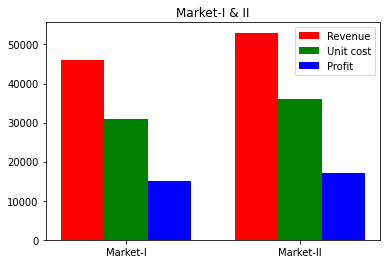
\includegraphics[width=\columnwidth]{solutions/su2021/45/FIGURE.png}
\caption{Revenue,Sales \& Profit Of Market-I \& II}
\label{matrix/2/45/fig:Profit}	
\end{figure}

  \item If A and B are square matrices of the same order such that AB=BA,then prove by indication that $AB^{n}=B^{n}A$.Further prove that $(AB)^{n}=A^{n}B^{n}$ for all $n \epsilon N$.\\
  Choose the correct answer in the following questions:\\
  \item If A=$\myvec{\alpha &\beta\\ \gamma &-\alpha}$ is such that $A^{2}=I$,then\\
  (A)$1+\alpha^{2}+\beta\gamma=0$ (B)$1-\alpha^{}2+\beta\gamma=0$\\
  (C)$1-\alpha^{2}-\beta\gamma=0$ (D)$1+\alpha^{2}-\beta\gamma=0$\\
\\
\solution
%
\begin{align}
    E(X) &= \frac{1}{\sqrt{2\pi}} \int_{-\infty}^{\infty} x e^{-\frac{x^2}{2}}dx\\
    &=0 \quad \brak{ \text{ odd function}}
\end{align}
\begin{align}
    E\brak{X^2}&= \frac{1}{\sqrt{2\pi}}\int_{-\infty}^{\infty} x^2
e^ {-\frac{x^2}{2}} dx \quad \brak{even function}\\
    &= \frac{2}{\sqrt{2\pi}} \int_{0}^{\infty} x^2 e^{-\frac{x^2}{2}} dx\\
    &= \frac{2}{\sqrt{2\pi}}\int_{0}^{\infty}\sqrt{2u}e^{-u} du \quad\brak{Let \frac{x^2}{2}= u}\\
    &= \frac{2}{\sqrt{\pi}} \int_{0}^{\infty} e^{-u} u^{\frac{3}{2}-1} du\\
    &= \frac{2}{\sqrt{\pi}} \Gamma\brak{{\frac{3}{2}}}\\
    &= \frac{1}{\sqrt{\pi}}\Gamma\brak{\frac{1}{2}} \\
    &= 1
\end{align}
where we have used the fact that
\begin{align}
\quad\because \Gamma(n)= (n-1)\Gamma(n-1); \Gamma\brak{\frac{1}{2}}=\sqrt{\pi}
\end{align}
%
Thus, the  variance is
\begin{align}
    \sigma^2 =  E\brak X^2 - E^2\brak X = 1
\end{align}

  \item If the matrix A is both symmetric and skew symmetric,then\\
  (A) A is a diagonal matrix \\
  (B) A is a zero matriz\\
  (C)A is a square matrix \\
  (D)None of these\\
  \\
\solution
If $\vec{A}$ is symmetric, then 
\begin{align}
\vec{A}^T =\vec{A}
\label{matrix/48/2.0.1}
\end{align}
If matrix A is skew symmetric, then
\begin{align}
\vec{A}^T = \vec{-A}
\label{matrix/48/2.0.2}
\end{align}
From  \eqref{matrix/48/2.0.1} and \eqref{matrix/48/2.0.2},
\begin{align}
\vec{A} &=\vec{-A}
\\
\implies 2\vec{A} &= 0
\\
\text{or, } \vec{A} &= 0
\end{align}
$\therefore $ $\vec{A}$ is zero matrix.


  \item If A is square matrix such that $A^{2}=A$,then $(I+A)^{3}-7A$ is equal to\\
  (A)A \\(B)I-A\\ (C)I\\ (D)3A
\\
\solution
%
\begin{align}
    E(X) &= \frac{1}{\sqrt{2\pi}} \int_{-\infty}^{\infty} x e^{-\frac{x^2}{2}}dx\\
    &=0 \quad \brak{ \text{ odd function}}
\end{align}
\begin{align}
    E\brak{X^2}&= \frac{1}{\sqrt{2\pi}}\int_{-\infty}^{\infty} x^2
e^ {-\frac{x^2}{2}} dx \quad \brak{even function}\\
    &= \frac{2}{\sqrt{2\pi}} \int_{0}^{\infty} x^2 e^{-\frac{x^2}{2}} dx\\
    &= \frac{2}{\sqrt{2\pi}}\int_{0}^{\infty}\sqrt{2u}e^{-u} du \quad\brak{Let \frac{x^2}{2}= u}\\
    &= \frac{2}{\sqrt{\pi}} \int_{0}^{\infty} e^{-u} u^{\frac{3}{2}-1} du\\
    &= \frac{2}{\sqrt{\pi}} \Gamma\brak{{\frac{3}{2}}}\\
    &= \frac{1}{\sqrt{\pi}}\Gamma\brak{\frac{1}{2}} \\
    &= 1
\end{align}
where we have used the fact that
\begin{align}
\quad\because \Gamma(n)= (n-1)\Gamma(n-1); \Gamma\brak{\frac{1}{2}}=\sqrt{\pi}
\end{align}
%
Thus, the  variance is
\begin{align}
    \sigma^2 =  E\brak X^2 - E^2\brak X = 1
\end{align}

\item Balance the following chemical equation.
\begin{align}
  \label{matrix/50/eq1}
NaOH + H_2SO_4 \xrightarrow{} Na_2SO_4  +  H_2O
\end{align}
\\
\solution
Let the balanced version of \eqref{matrix/50/eq1} be
\begin{align}
   x_{1}NaOH + x_{2}H_2SO_4 \xrightarrow{} 
   x_{3}Na_2SO_4 + x_{4}H_2O \label{matrix/50/eq2}
\end{align}
which results in the following equations:
\begin{align}
    (x_{1}-2x_{3}) Na= 0\\
    (x_{1}+4x_{2}-4x_{3}-x_{4}) O= 0\\
    (x_{1}+2x_{2}-2x_{4}) H=0\\
    (x_{2}-x_{3}) S= 0
\end{align}
which can be expressed as
\begin{align}
    x_{1}+ 0.x_{2}- 2x_{3}+ 0.x_{4} = 0\\
    x_{1}+ 4x_{2}- 4x_{3}- x_{4} = 0\\
    x_{1}+ 2x_{2}+ 0.x_{3}- 2x_{4} = 0\\
    0.x_{1}+ x_{2}- x_{3}+ 0.x_{4} = 0
\end{align}
resulting in the matrix equation
\begin{align}
    \myvec{1 & 0 & -2 & 0\\
           1 & 4 & -4 & -1\\
           1 & 2 & 0 & -2\\
           0 & 1 & -1 & 0}\vec{x}
           =\vec{0}    \label{matrix/50/eq3}
\end{align}
where,
\begin{align}
   \vec{x}= \myvec{x_{1}\\x_{2}\\x_{3}\\x_{4}}
\end{align}
\eqref{matrix/50/eq3} can be reduced as follows:
\begin{align}
    \myvec{1 & 0 & -2 & 0\\
           1 & 4 & -4 & -1\\
           1 & 2 & 0 & -2\\
           0 & 1 & -1 & 0}
    \xleftrightarrow[R_{3}\leftarrow R_3-R_{1}]{R_{2}\leftarrow R_2- R_1}
    \myvec{1 & 0 & -2 & 0\\
           0 & 4 & -2 & -1\\
           0 & 2 & 2 & -2\\
           0 & 1 & -1 & 0}\\
    \xleftrightarrow{R_2 \leftarrow \frac{R_2}{4}}
    \myvec{1 & 0 & -2 & 0\\
          0 & 1 & -\frac{1}{2} & -\frac{1}{4}\\
          0 & 2 & 2 & -2\\
          0 & 1 & -1 & 0}\\
    \xleftrightarrow[R_4 \leftarrow R_4 - R_2]{R_3 \leftarrow R_3 - 2R_2}
    \myvec{1 & 0 & -2 & 0\\
           0 & 1 & -\frac{1}{2} & -\frac{1}{4}\\
           0 & 0 & 3 & -\frac{3}{2}\\
           0 & 0 & -\frac{1}{2} & \frac{1}{4}}\\
    \xleftrightarrow{R_3 \leftarrow \frac{R_3}{3}}
    \myvec{1 & 0 & -2 & 0\\
           0 & 1 & -\frac{1}{2} & -\frac{1}{4}\\
           0 & 0 & 1 & -\frac{1}{2}\\
           0 & 0 & -\frac{1}{2} & \frac{1}{4}}\\
    \xleftrightarrow[R_{4}\leftarrow R_4+\frac{R_3}{2}]{R_{2}\leftarrow R_2+ \frac{R_3}{2}}
    \myvec{1 & 0 & -2 & 0\\
           0 & 1 & 0 & -\frac{1}{2}\\
           0 & 0 & 1 & -\frac{1}{2}\\
           0 & 0 & 0 & 0}\\
    \xleftrightarrow{R_1 \leftarrow R_1+2R_3}
    \myvec{1 & 0 & 0 & -1\\
           0 & 1 & 0 & -\frac{1}{2}\\
           0 & 0 & 1 & -\frac{1}{2}\\
           0 & 0 & 0 & 0}
\end{align}
Thus,
\begin{align}
    x_1=x_4, x_2= \frac{1}{2}x_4, x_3=\frac{1}{2}x_4\\
    \implies \quad\vec{x}= x_4\myvec{1\\ \frac{1}{2}\\ \frac{1}{2}\\1} 
\end{align} 
by substituting $x_4= 2$
\begin{align}
    \vec{x}=\myvec{2\\1\\1\\2}
\end{align}
Hence, \eqref{matrix/50/eq2} finally becomes
\hfill\break
%\vspace{5mm}  finally becomes
\begin{align}
    2 NaOH + H_2SO_4 \xrightarrow{} 
    Na_2SO_4 + 2 H_2O
\end{align}

\item Balance the following chemical equation
\begin{align}\label{1}
    BaCl_2 + H_2SO_4 \xrightarrow{} BaSO_4 + HCl
\end{align}
    \item If A=\myvec{1 &2 &3\\2 &3 &1} and B=\myvec{3 &-1 &3\\-1 &0 &2}, then find 2A-B.\\
    \item If A=\myvec{8 &0\\4 &-2\\3 &6} and B=\myvec{2 &-2\\4 &2\\-5 &1}, then find the matrix X, such that 2A+3X=5B.\\
    \item Find X and Y, if X+Y=\myvec{5 &2\\0 &9} and \\X-Y=\myvec{3 &6\\0 &-1}.\\
    \item Find the values of x and y from the following equation:\\
    2\myvec{x &5\\7 &y-3} + \myvec{3 &-4\\1 &2} = \myvec{7 &6\\15 &14}\\
     
    

\item     Two farmers Ramkishan and Gurcharan Singh cultivate only three varieties of rice namely Basmati, Permal and Naura. The sale (in Rupees) of these varieties of rice by both the farmers in the month of September and October are given by the following matrices $\vec{A}$ and $\vec{B}$ .

\begin{center}
September Sales(in Rupees)
\end{center}
\begin{align}
    \vec{A}=
    \begin{blockarray}{cccc}
    \text{Basmati} & \text{Permal} & \text{Naura} \\
    \begin{block}{(ccc)(c)}
    10000 & 20000 & 30000 & \text{Ramkishan}\\
    50000 & 30000 & 10000 & \text{Gurucharan} \\
    \end{block}
    \end{blockarray}
\end{align}

\begin{center}
October Sales(in Rupees)
\end{center}
\begin{align}
    \vec{B} =
    \begin{blockarray}{cccc}
    \text{Basmati} & \text{Permal} & \text{Naura} \\
    \begin{block}{(ccc)(c)}
    5000 & 10000 & 6000 & \text{Ramkishan}\\
    20000 & 10000 & 10000 & \text{Gurucharan} \\
    \end{block}
    \end{blockarray}
\end{align}

\begin{enumerate}
    \item Find the combined sales in September and October for each farmer in each variety.
    \item Find the decrease in sales from September to October.
    \item If both farmers receive 2\% profit on gross sales, compute the profit for each farmer and for each variety sold in October.
\end{enumerate}
%
\solution

The given system of inequality can be written in matrix form as
\begin{align}
    \myvec{-1 & -2  \\ -1 & 1 \\ 1 & 1\\ 1 & 0 \\ 0 & 1}\vec{x} \succeq \myvec{-10\\0\\1\\0\\0}
\end{align}
which can be further simplified into 
\begin{align}
    \myvec{-1 & -2 \\ 1 & 0 \\ 0&1}\vec{x} \succeq \myvec{-10\\\frac{-1}{2}\\\frac{-1}{2}}
\end{align}
Let the surplus vector be
\begin{align}
    \vec{u} &= \myvec{u_1\\u_2} \succeq 0
\end{align}
\begin{enumerate}
    \item 
    \begin{align}
        \myvec{-1 & -2 \\ 1 & 0}\vec{x} &\succeq \myvec{-10 \\ \frac{-1}{2}}
        \\
        \implies  \myvec{-1 & -2 \\ 1 & 0}\vec{x} &= \myvec{-10 \\ \frac{-1}{2}} + \vec{u}
    \end{align}
    resulting in 
    \begin{align}
        \vec{x} &= \myvec{-1 & -2 \\ 1 & 0}^{-1}\myvec{-10 \\\frac{-1}{2}} + \myvec{-1 & -2 \\ 1 & 0}^{-1}\vec{u}
        \\
        \implies \vec{x} &= \myvec{\frac{1}{2} \\ \frac{19}{4}} + \myvec{0&1\\ \frac{-1}{2}&\frac{-1}{2}}\vec{u}   \label{ineq/58/eq1}
    \end{align}
    \item 
    \begin{align}
        \myvec{-1& -2 \\ 0 & 1}\vec{x} &\succeq \myvec{-10 \\ \frac{-1}{2}}
        \\
        \implies  \myvec{-1& -2 \\ 0 & 1}\vec{x} &= \myvec{-10 \\ \frac{-1}{2}} + \vec{u}
    \end{align}
    resulting in 
    \begin{align}
        \vec{x} &= \myvec{-1& -2 \\ 0 & 1}^{-1}\myvec{-10 \\ \frac{-1}{2}} + \myvec{-1& -2 \\ 0 & 1}^{-1}\vec{u}
        \\
        \implies \vec{x} &= \myvec{9\\\frac{1}{2}} + \myvec{-1& -2 \\ 0 & 1}\vec{u} \label{ineq/58/eq2}
    \end{align}
\end{enumerate}
Now,solution region which is common to regions of eq. \eqref{ineq/58/eq1} and eq. \eqref{ineq/58/eq2},is given by
\begin{align}
    \boxed{\vec{x} = \myvec{\frac{1}{2}\\\frac{1}{2}}+\myvec{0&1\\\frac{-1}{2}&1}\vec{u}}
\end{align}
%
\begin{figure}[!ht]
\centering
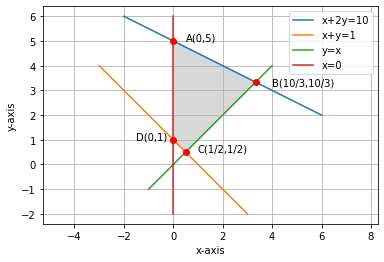
\includegraphics[width=\columnwidth]{solutions/su2021/2/58/Figures/Figure_2.58.png}
\caption{Graphical Solution}
\label{ineq/58/fig:fig1}	
\end{figure}

\begin{figure}[!ht]
\centering
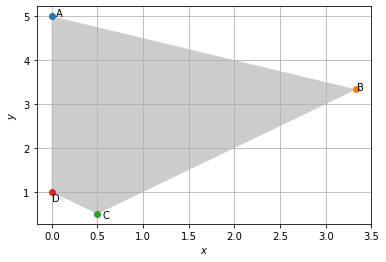
\includegraphics[width=\columnwidth]{solutions/su2021/2/58/Figures/2.58(2).png}
\caption{Magnified Solution region}
\label{ineq/58/fig:fig2}	
\end{figure}


   
    \item  Find AB, if A=\myvec{6 &9\\2 &3} and B=\myvec{2 &6 &0\\7 &9 &8}.\\
    \item  If A=\myvec{1 &-2 &3\\-4 &2 &5\\} and B=\myvec{2 &3\\4 &5\\2 &1}, then find AB,BA.Show that AB$\neq$BA

   
     \item If A=\myvec{1 &0 \\0 &-1} and  B=\myvec{0 &1\\1 &0}, then find AB,BA. Show that AB$\neq$BA\\
     
   
    \item Find AB, if A=\myvec{0 &-1\\0 &2} and B=\myvec{3 &5\\0 &0}\\
     
   
    \item If A=\myvec{1 &1 &-1\\2 &0 &3\\3 &-1 &2}, B=\myvec{1 &3\\0 &2\\-1 &4} and C=\myvec{1 &2 &3 &-4\\2 &0 &-2 &1}, find\\A(BC),(AB)C and show that (AB)C=A(BC) \\   
    
     \item If A=\myvec{0 &6 &7\\-6 &0 &8\\7 &-8 &0}, B=\myvec{0 &1 &1\\1 &0 &2\\1 &2 &0},C=\myvec{2\\-2\\3}\\Calculate AC,BC and (A+B)C=AC+BC\\

    \item If A=$\myvec{1 &2 &3\\3 &-2 &1\\4 &2 &1}$,then show that $A^3-23A-40I=0$
  \\  
  \solution
  Given that $\vec{A}$ =$\myvec{1&2&3\\3&-2&1\\4&2&1}$.
\begin{enumerate}
\item \textbf{The Characteristic equation} is given by:
\begin{align}
  \implies  \abs{\vec{A}-\lambda\vec{I}}&=0
    \\
    \implies \mydet{1-\lambda&2&3\\3&-2-\lambda&1\\4&2&1-\lambda}&=0
    \end{align}
\begin{multline}
   \implies\brak{1-\lambda}\brak{\brak{-2-\lambda}\brak{1-\lambda}-2}
   \\
   -2\brak{3\brak{1-\lambda}-4}+3\brak{6+4\brak{2+\lambda}}=0
\end{multline}
\begin{align}
 \implies   \lambda^3-23\lambda-40=0
\end{align}
The above equation is similar to equation to be proved.
\item According to \textbf{Cayley-Hamilton Theorem:} 
\\
Every square matrix satisfies its own
\\\textbf{characteristic equation}.
\begin{align}
\therefore    \vec{A}^3-23\vec{A}-40\vec{I}=0
\end{align}
Hence Proved.
\end{enumerate}
    
    
\item In a legislative assembly election, a political
group hired a public relations firm to promote
its candidate in three ways: telephone, house
calls, and letters. The cost per contact (in paise)
is given in matrix $\vec{A}$ as
\begin{center}
Cost per Contact(in Paise)
\end{center}
\begin{align}
    \vec{A}=
    \begin{blockarray}{cc}
    \text{cost}\\
    \begin{block}{(c)(c)}
    40 &\text{Telephone}\\
    100&\text{Housecall} \\
    50&\text{Letter}\\
    \end{block}
    \end{blockarray}
\end{align}
The number of contacts of each type made in
two cities X and Y is given by matrix $\vec{B}$
\begin{align}
    \vec{B} =
    \begin{blockarray}{cccc}
    \text{Telephone} & \text{Housecall} & \text{Letter} \\
    \begin{block}{(ccc)(c)}
    1000 & 500 & 5000 & \text{X}\\
    3000 & 1000 & 10000 & \text{Y} \\
    \end{block}
    \end{blockarray}
\end{align}
Find the total
amount spent by the group in the two cities
X and Y
%
\solution

The total amount spent is given by=

    \begin{multline}
    \vec{B}\vec{A}\\
    =\myvec{1000&500&5000\\3000&1000&10000}\myvec{40\\100\\50}\\
    =\myvec{40000+50000+250000\\120000+100000+500000}\\
    \begin{blockarray}{cc}
    \text{TotalCost} \\
    \begin{block}{(c)(c)}
    340000&\text{X}\\
    720000&\text{Y}\\
    \end{block}
    \end{blockarray}
    \end{multline}
$\therefore$ the total amount spent in city X and city Y is 3400 and 7200 Rupees respectively.  See Fig. \ref{matrix/64fig:Profit}	
%
\begin{figure}[!ht]
\centering
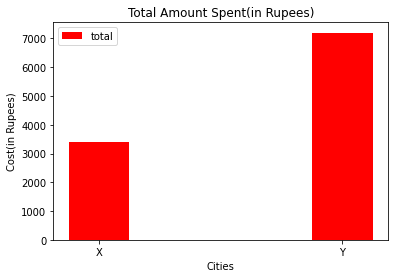
\includegraphics[width=\columnwidth]{solutions/su2021/64/figure8.png}
\caption{Total Amount Spent by the group in cities X and Y}
\label{matrix/64fig:Profit}	
\end{figure}


\item If A=$\myvec{3 &\sqrt{3} &2\\4 &2 &0}$ and B=$\myvec{2 &-1 &2\\1 &2 &4}$, verify that\\
(i) $(A^{'})^{'}=A$\\ (ii)$(A+B)^{'}=A^{'}+B^{'}$,\\ (iii) $(kB)^{'}=kB^{'}$,where k is any constant.\\
\item If A=$\myvec{-2\\4 \\5}$,B=$\myvec{1 &3 &-6}$, verify that $(AB)^{'}=B^{'}A^{'}$\\
\item Express the matrix B=$\myvec{2 &-2 &-4\\-1 &3 &4\\1 &-2 &-3}$ as the sum of a symmetric and a skew symmetric matrix.\\
\solution
  We obtain the vertices of the rhombus as follows
\begin{align}
\vec{A} = \myvec{-3\\0},
\vec{B} = \myvec{0\\-3.5},
\vec{C} = \myvec{3\\0},
\vec{D} = \myvec{0\\3.5}
\end{align}
which are plotted in Fig. \ref{quad/45/fig:Rhombus ABCD}.
%
\begin{figure}[ht!]
\centering
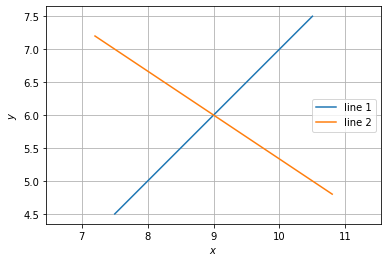
\includegraphics[width=\columnwidth]{solutions/quad/45/figure2.png}
\caption{Rhombus ABCD}
\label{quad/45/fig:Rhombus ABCD}
\end{figure}

  
\item By using elementary operations,find the inverse of the matrix\\
A=$\myvec{1 &2\\2 &-1}$.\\
\item Obtain the inverse of the following matrix using elementary operations\\
A=$\myvec{0 &1 &2\\1 &2 &3\\3 &1 &1}$.\\
\solution
  \begin{enumerate}
    \item Given that
    \begin{align}
    \vec{A}& =\myvec {0 & 1 & 2\\1 & 2 & 3\\3 & 1 & 1}
    \end{align}
     The augmented matrix $[A | I]$ is as given below:- 
    \begin{align}
    \myvec{0 & 1 & 2 & \vrule & 1 & 0 & 0\\1 & 2 & 3 & \vrule & 0 & 1 & 0\\3 & 1 & 1 & \vrule & 0 & 0 & 1}
    \end{align}
    We apply the elementary row operations on $[A | I]$ as follows :-
    \begin{align}
    [A | I] = \myvec{0 & 1 & 2 & \vrule & 1 & 0 & 0\\1 & 2 & 3 & \vrule & 0 & 1 & 0\\3 & 1 & 1 & \vrule & 0 & 0 & 1}
    \\
    \xleftrightarrow{R_1\leftrightarrow R_2}   
    \myvec{1 & 2 & 3 & \vrule & 0 & 1 & 0\\0 & 1 & 2 & \vrule & 1 & 0 & 0\\3 & 1 & 1 & \vrule & 0 & 0 & 1}
    \\
    \xleftrightarrow{R_3\leftarrow R_3-3R_1}   
    \myvec{1 & 2 & 3 & \vrule & 0 & 1 & 0\\0 & 1 & 2 & \vrule & 1 & 0 & 0\\0 & -5 & -8 & \vrule & 0 & -3 & 1}
    \\
    \xleftrightarrow{R_1\leftarrow R_1-2R_2}  
    \myvec{1 & 0 & -1 & \vrule & -2 & 1 & 0\\0 & 1 & 2 & \vrule & 1 & 0 & 0\\0 & -5 & -8 & \vrule & 0 & -3 & 1}
    \\
    \xleftrightarrow{R_3\leftarrow R_3+5R_2}  
    \myvec{1 & 0 & -1 & \vrule & -2 & 1 & 0\\0 & 1 & 2 & \vrule & 1 & 0 & 0\\0 & 0 & 2 & \vrule & 5 & -3 & 1}
    \\
    \xleftrightarrow{R_3\leftarrow R_3/2}
    \myvec{1 & 0 & -1 & \vrule & -2 & 1 & 0\\ 0 & 1 & 2 & \vrule & 1 & 0 & 0\\0 & 0 & 1 &\vrule &\frac{5}{2} &\frac{-3}{2} &\frac{1}{2}}
    \\
    \xleftrightarrow{R_1\leftarrow R_1+R_3}
    \myvec{1 & 0 & 0 & \vrule & \frac{1}{2} & \frac{-1}{2} & \frac{1}{2}\\ 0 & 1 & 2 & \vrule & 1 & 0 & 0\\0 & 0 & 1 &\vrule &\frac{5}{2} &\frac{-3}{2} &\frac{1}{2}}
    \\
    \xleftrightarrow{R_2\leftarrow R_2-2R_3}
    \myvec{1 & 0 & 0 & \vrule & \frac{1}{2} & \frac{-1}{2} & \frac{1}{2}\\ 0 & 1 & 0 & \vrule & -4 & 3 & -1\\0 & 0 & 1 &\vrule &\frac{5}{2} &\frac{-3}{2} &\frac{1}{2}}
    \end{align}
    By performing elementary transformations on augmented matrix$ [A | I]$ , we obtained the augmented matrix in the form $ [I | A]$. 
    Hence we can conclude that the matrix A is invertible and inverse of the matrix is:-
    \begin{align}
    \therefore\vec{A^{-1}}=\myvec { \frac{1}{2} & \frac{-1}{2} & \frac{1}{2} \\  -4 & 3 & -1\\ \frac{5}{2} &\frac{-3}{2} &\frac{1}{2}}
    \end{align}
    \item QR decomposition of  \myvec{0  & 1 & 3 \\ 1 & 2 & 3 \\ 2 & 3 & 1}
    \\
     Let us use the Gram-schmidt approach to obtain QR decomposition of$ \vec{A}$. Consider rows vectors say $\vec{a_1}$,$\vec{a_2}$ and $\vec{a_3}$ of $\vec{A}$  which is given by
    \begin{align}
    \vec{a_1}=\myvec{0 & 1 & 2}\label{matrix/69/eq1}\\
    \vec{a_2}=\myvec{1 & 2 & 3}\label{matrix/69/eq2}\\
    \vec{a_3}=\myvec{3 & 1 & 1}\label{matrix/69/eq3}
    \end{align}
    we can express these as 
    \begin{align}
    \vec{u_1}&=\vec{a_1}=\myvec{0 & 1 & 2}\label{matrix/69/eq4}\\
    \vec{e_1}&=\frac{\vec{u_1}}{\norm{\vec{u_1}}}\\
    \vec{e_1}&=\frac{\myvec{0 & 1 & 2}}{\sqrt{0+1+4}}\\
    \vec{e_1}&=\myvec{0 & \frac{1}{\sqrt{5}} & \frac{2}{\sqrt{5}}}\\
    \vec{u_2}&=\vec{a_2}-(\vec{a_2}\vec{e_1})\vec{e_1}\\
    &=\myvec{1 & 2 & 3}-(\myvec{1 & 2 & 3}\myvec{0 & \frac{1}{\sqrt{5}} & \frac{2}{\sqrt{5}}})\myvec{0 & \frac{1}{\sqrt{5}} &  \frac{2}{\sqrt{5}}}\\
    &=\myvec{1 & \frac{2}{5} & \frac{-1}{5}}\\
    \vec{e_2}&=\frac{\vec{u_2}}{\norm{\vec{u_2}}}=\frac{\myvec{1 & \frac{2}{5} & \frac{-1}{5}}}{\sqrt{1+\frac{4}{25}+\frac{1}{25}}}\\
    \vec{e_2}&=\myvec{\frac{5}{\sqrt{30}} & \frac{2}{\sqrt{30}} &\frac{-1}{\sqrt{30}}}\\
    \vec{u_3}&=\vec{a_3}-(\vec{a_3}\vec{e_1})\vec{e_1}-(\vec{a_3}\vec{e_2})\vec{e_2}
    \\
    \vec{u_3}&=\myvec{\frac{1}{3} & \frac{-2}{3} &\frac{1}{3}}\\
    \vec{e_3}&=\frac{\vec{u_3}}{\norm{\vec{u_3}}}\\
    &=\frac{\myvec{\frac{1}{3} & \frac{-2}{3} & \frac{1}{4}}}{\sqrt{\frac{1}{9}+\frac{4}{9}+\frac{1}{9}}}\\
    \vec{e_3}&=\myvec{\frac{1}{\sqrt{6}} & \frac{-2}{\sqrt{6}} &\frac{1}{\sqrt{6}}}
    \end{align}
    Thus,
    \begin{align}
     \vec{Q}&=(e_1|e_2|----|e_n)\\
     &=\myvec{0 & \frac{5}{\sqrt{30}} & \frac{1}{\sqrt{6}}\\\frac{1}{\sqrt{5}} & \frac{2}{\sqrt{30}} & \frac{-2}{\sqrt{6}}\\\frac{2}{\sqrt{5}} & \frac{-1}{\sqrt{30}} & \frac{1}{\sqrt{6}}}\label{matrix/69/eq5}      
    \end{align}
    Then
    \begin{align}
      \vec{R}&=\myvec{a_1e_1 & a_2e_1 & a_3e_1\\ 0 & a_2e_2 & a_3e_2\\0 & 0 & a_3e_3}\\
      &=\myvec{\frac{5}{\sqrt{5}} & \frac{8}{\sqrt{5}} & \frac{3}{\sqrt{5}}\\0 &  \frac{6}{\sqrt{30}} & \frac{16}{\sqrt{30}}\\0 & 0 & \frac{2}{\sqrt{6}}}\label{matrix/69/eq6} 
      \end{align}
    From equations \eqref{matrix/69/eq5} and \eqref{matrix/69/eq6} the obtained $\vec{Q} \vec{R}$ Decomposition is
    \begin{align}
     \myvec{0  & 1 & 3 \\ 1 & 2 & 3 \\ 2 & 3 & 1}&= \myvec{0 & \frac{5}{\sqrt{30}} & \frac{1}{\sqrt{6}}\\\frac{1}{\sqrt{5}} & \frac{2}{\sqrt{30}} & \frac{-2}{\sqrt{6}}\\\frac{2}{\sqrt{5}} & \frac{-1}{\sqrt{30}} & \frac{1}{\sqrt{6}}}\myvec{\frac{5}{\sqrt{5}} & \frac{8}{\sqrt{5}} & \frac{3}{\sqrt{5}}\\0 &  \frac{6}{\sqrt{30}} & \frac{16}{\sqrt{30}}\\0 & 0 & \frac{2}{\sqrt{6}}} 
    \end{align}
    \end{enumerate}

\item Find P$^{-1}$, if it exists, given \\
P=$\myvec{10 &-2\\-5 &1}$.\\
\item If A=$\myvec{\cos\theta &\sin\theta\\ \-sin\theta &\cos\theta}$,\\then prove that $A^{n}=\myvec{\cos\theta &\sin n\theta\\\-sin n\theta &\cos n\theta}$, n $\in$ N.\\
\item If A and B are symmetric matrices of the same order, then show that AB is symmetric if and only if A and B commute,that AB = BA.\\
\item Let A=$\myvec{2 &-1\\3 &4}$, B=$\myvec{5 &2\\7 &4}$, C=$\myvec{2 &5\\3 &8}$. Find a matrix D such that CD-AB=0. 
\item Find the values of a,b,c and d from the equations: \myvec{a-b &2a+c\\2a-b &3c+d} = \myvec{-1 &5\\0 &13}
\item Show that\\
(i)$\myvec{5 &-1\\6 &7}\myvec{2 &1\\3 &4}\neq\myvec{2 &1\\3 &4}\myvec{5 &-1\\6 &7}$
\\
(ii)$\myvec{1 &2 &3\\0 &1 &0\\1 &1 &0}\myvec{-1 &1 &0\\0 &-1 &1\\2 &3 &4}\neq \myvec{-1 &1 &0\\0 &-1 &1\\2 &3 &4}\myvec{1 &2 &3\\0 &1 &0\\1 &1 &0}$\\
\item If A=\myvec{3 &-2\\4 &-2} and I=\myvec{1 &0\\0 &1},find k\\
 so that $A^2=kA-2I$\\
  \item Find the matrix X so that\\ X\myvec{1 &2 &3\\4 &5 &6}=\myvec{-7 &-8 &-9\\2 &4 &6}\\
\item (i) $\begin{vmatrix}a-b-c& 2a& 2a \\ 2b& b-c-a& 2b \\ 2c& 2c& c-a-b\end{vmatrix}$= $(a+b+c)^3$\\
(ii) $\begin{vmatrix}x+y+2z&x&y \\ z&y+z+2x&y \\ z&x&z+x+2y\end{vmatrix}$=$2(x+y+z)^3$
\item $\begin{vmatrix}1&x&x^2 \\ x^2&1&x \\ x&x^2&1\end{vmatrix}$=$(1-x^3)^2$ 
\item $\begin{vmatrix}1+a^2-b^2&2ab&-2b \\ 2ab&1-a^2+b^2&2a \\ 2b&-2a&1-a^2-b^2\end{vmatrix}$=$(1+a^2+b^2)^3$
\item Let 
A=$\begin{bmatrix}
1&\sin\theta&1 \\ -\sin\theta&1&\sin\theta \\ -1&-\sin\theta&1
\end{bmatrix},$ 
where $0\leq \theta \leq 2\Pi.$ Then
\begin{enumerate}
\item Det(A)=0
\item Det(A)$\in(2,\infty)$
\item Det(A)$\in (2,4)$
\item Det(A)$\in [2,4]$
\end{enumerate}
\item $\begin{vmatrix}
1&1+p&1+p+q \\ 2&3+2p&4+3p+2q \\ 3&6+3p&10+6p+3q
\end{vmatrix}$=1\\
\item $\begin{vmatrix}\sin\alpha&\cos\alpha&\cos(\alpha+\delta) \\ \sin\beta&\cos\beta&\cos(\beta+\delta) \\ \sin\gamma&\cos\gamma&\cos(\gamma+\delta)\end{vmatrix}$=0\\
\item Solve the system of equations \\$\frac{2}{x}+\frac{3}{y}+\frac{10}{z}=4$\\$\frac{4}{x}-\frac{6}{y}+\frac{5}{z}=1$\\$\frac{6}{x}+\frac{9}{y}-\frac{20}{z}=2$\\
\item If a,b,c are in A.P, then the determinant\\
 $\begin{vmatrix}
x+2&x+3&x+2a \\ x+3&x+4&x+2b \\x+4&x+5&x+2c
\end{vmatrix}$ is 
\begin{enumerate}
\item 0
\item 1
\item x
\item 2x
\end{enumerate}
\item If x,y,z are nonzero real numbers, then the inverse of matrix 
A=$\begin{bmatrix}
x&0&0 \\ 0&y&0 \\ 0&0&z
\end{bmatrix}$ is 
\begin{enumerate}
\item $\begin{bmatrix} x^{-1}&0&0 \\ 0&y^{-1}&0 \\ 0&0&z^{-1} \end{bmatrix}$ 
\item $xyz\begin{bmatrix} x^{-1}&0&0 \\ 0&y^{-1}&0 \\ 0&0&z^{-1} \end{bmatrix}$ 
\item $\frac{1}{xyz}\begin{bmatrix} x&0&0 \\ 0&y&0 \\ 0&0&z \end{bmatrix}$ 
\item $\frac{1}{xyz}\begin{bmatrix} 1&0&0 \\ 0&1&0 \\ 0&0&1 \end{bmatrix}$ 
\end{enumerate}
\textbf{Examine the consistency of the system of given Equations.}
\item 
$\begin{alignedat}[t]{2}
x+2y&=2 
\\
2x+3y&=3 
\end{alignedat}$
\item $\begin{alignedat}[t]{2}
2x-y&=5 
\\
x+y&=4 
\end{alignedat}$
\item Evaluate the determinant
$\begin{vmatrix}0&a&-b\\-a&0&-c\\b&c&0\end{vmatrix}=0$
\\
Find the inverse and QR decomposition of the following.
  \item \myvec{2 &1\\1 &1}\\
  \item\myvec{1 &3\\2 &7}\\
  \item\myvec{2 &3\\5 &7}\\
  \item\myvec{2 &1\\7 &4}\\
  \item \myvec{2 &5\\1 &3}\\
  \item \myvec{3 &1\\5 &2}\\
  \item \myvec{4 &5\\3 &4}\\
  \item \myvec{3 &10\\2 &7}\\
  \item \myvec{3 &-1\\-4 &2}\\
  \item \myvec{2 &-6\\1 &-2}\\
  \item \myvec{6 &-3\\-2 &1}\\
  \item \myvec{2 &-3\\-1 &2}\\
  \item \myvec{2 &1\\4 &2}\\
\item Find the QR decomposition of 
\begin{align}
\vec{A}=\myvec{8&5\\3&2} \label{eq:solutions/decomp/2/29/eq:1}
\end{align}
%%
%
\item Find the QR decomposition of 
\begin{align}
\vec{A}=\myvec{2&5\\1&4} \label{eq:solutions/decomp/2/30/1}
\end{align}

%    \end{document}    



\end{enumerate}

%
%
\end{document}


